%Przykładowy plik ułatwiający złożenie projektu dyplomowego inżynierskiego.
%UWAGA: Generowany napis na stronie tytułowej o treści PROJEKT DYPLOMOWY INŻYNIERSKI został zaproponowany przeze mnie i nie jest, póki co, potwierdzony przez władze wydziału. Przed ostatecznym oddaniem tak złożonej pracy należy upewnić się jaka powinna być treść tego napisu. W momencie gdy uzyskam informację na temat treści tego napisu, dokonam niezbędnych zmian w źródłach.

\documentclass[en,printmode]{mgr}
%opcje klasy dokumentu mgr.cls zostały opisane w dołączonej instrukcji

%poniżej deklaracje użycia pakietów, usunąć to co jest niepotrzebne
%\usepackage{polski} %przydatne podczas składania dokumentów w j. polskim
\usepackage[utf8]{inputenc}
\usepackage[T1]{fontenc} %poprawne składanie polskich czcionek
%pakiety do grafiki
\usepackage{graphicx}
\usepackage{subcaption}
\usepackage{psfrag}

%pakiety dodające dużo dodatkowych poleceń matematycznych
\usepackage{amsmath}
\usepackage{amsfonts}

%pakiety wspomagające i poprawiające składanie tabel
\usepackage{supertabular}
\usepackage{array}
\usepackage{tabularx}
\usepackage{hhline}
\usepackage{multirow}
\usepackage{indentfirst}
\usepackage{enumitem}
\usepackage{listings}
\usepackage{float}
\usepackage{color} %red, green, blue, yellow, cyan, magenta, black, white
\definecolor{mygreen}{RGB}{28,172,0} % color values Red, Green, Blue
\definecolor{mylilas}{RGB}{170,55,241}
\usepackage[colorinlistoftodos]{todonotes}
\usepackage{breqn}

\lstset{language=Matlab,%
	%basicstyle=\color{red},
	breaklines=true,%
	morekeywords={matlab2tikz},
	keywordstyle=\color{blue},%
	morekeywords=[2]{1}, keywordstyle=[2]{\color{black}},
	identifierstyle=\color{black},%
	stringstyle=\color{mylilas},
	commentstyle=\color{mygreen},%
	showstringspaces=false,%without this there will be a symbol in the places where there is a space
	numbers=left,%
	numberstyle={\tiny \color{black}},% size of the numbers
	numbersep=9pt, % this defines how far the numbers are from the text
	emph=[1]{for,end,break},emphstyle=[1]\color{red}, %some words to emphasise
	%emph=[2]{word1,word2}, emphstyle=[2]{style},    
}

\newcommand{\floor}[1]{\left\lfloor #1 \right\rfloor}
\usepackage[justification=centering]{caption}

%pakiet wypisujący na marginesie etykiety równań i rysunków zdefiniowanych przez \label{}, chcąc wygenerować finalną wersję dokumentu wystarczy usunąć poniższą linię
%\usepackage{showlabels}


%definicje własnych poleceń
\newcommand{\R}{I\!\!R} %symbol liczb rzeczywistych, działa tylko w trybie matematycznym
\newtheorem{theorem}{Twierdzenie}[section] %nowe otoczenie do składania twierdzeń

%dane do złożenia strony tytułowej
\title{ }
\engtitle{Problems of software implementation of SDR radio in programmable logic structures}
\author{Karol Szpila}
\supervisor{\vfil Ph.D., D.Sc. Grzegorz Budzyń\\
\\ Institute of Telecommunications, Teleinformatics and Acoustics (I-28)}
%\guardian{dr hab. inż. Imię Nazwisko Prof. PWr, I-6} %nie używać jeśli opiekun jest tą samą osobą co prowadzący pracę

%\date{2008} %standardowo u dołu strony tytułowej umieszczany jest bieżący rok, to polecenie pozwala wstawić dowolny rok

%poniżej jest lista kierunków i specjalności na wydziale elektroniki, należy wybrać właściwe lub dopisać jeśli nie ma odpowiednich
\field{Elektronika (EKA)}
\specialisation{Advanced Applied Electronics(AAE)}
%\specialisation{Robotyka (ARR)}
%\specialisation{Komputerowe sieci sterowania (ARK)}
%\specialisation{Systemy informatyczne w automatyce (ASI)}
%\specialisation{Komputerowe systemy zarządzania \\procesami produkcyjnymi (ARS)}
%\field{Elektronika i telekomunikacja (EIT)}
%\specialisation{Akustyka (ETA)}
%\specialisation{Aparatura elektroniczna (EAE)}
%\specialisation{Elektroniczne i komputerowe \\systemy automatyki (ESA)}
%\specialisation{Zastosowania inżynierii komputerowej \\w technice (EZI)}
%\specialisation{Inżynieria dźwięku (EID)}
%\specialisation{Elektronika stosowana \\i optokomunikacja (TEO)}
%\specialisation{Telekomunikacyjne sieci szerokopasmowe (TSS)}
%\specialisation{Teleinformatyczne sieci mobilne (TSM)}
%\specialisation{Sygnały w telekomunikacji cyfrowej (TSC)}
%\specialisation{Teleinformatyczne systemy rozsiewcze (TSR)}
%\field{Informatyka (INF)}
%\specialisation{Systemy informatyki w medycynie \\i technice (IMT)}
%\specialisation{Inżynieria systemów informatycznych (INS)}
%\specialisation{Inżynieria internetowa (INT)}
%\specialisation{Systemy i sieci komputerowe (ISK)}
%\field{Teleinformatyka (TIN)}
%\specialisation{Teleinformatyka (TIN)}

%tutaj zaczyna się właściwa treść dokumentu
\begin{document}
%\bibliographystyle{plabbrv} %tylko gdy używamy BibTeXa, ustawia polski styl bibliografii

\maketitle %polecenie generujące stronę tytułową
%\dedication{6cm}{To jest przykładowa treść opcjonalnej dedykacji, należy ją zmienić lub usunąć w całości polecenie \texttt{$\backslash$dedication}}

\chapter*{Nomenclature}
\begin{table}[!htb]
\begin{tabular}{ll}
$ADC$  & Analog to Digital Converter   \\
$ASIC$ & Application-Specific Integrated Circuit \\
$DAC$  & Digital to Analog Converter   \\
$DBIQIM$ & Double Branch IQ Imbalance Model \\
$CPU$  & Central Processing Unit \\
$FIR$  & Finite Impulse Response \\ 
$FPGA$ & Field Programmable Gate Array \\
$IF$   & Intermediate Frequency \\
$IQ$   & In-phase Quadrature \\
$LO$   & Local Oscillator \\
$LSB$  & Lower Side Band \\
$SDR$  & Software Defined Radio \\
$PLL$  & Phase Locked Loop \\
$RF$   & Radio Frequency \\
$SBIQIM$ & Single Branch IQ Imbalance Model \\
$SoC$  & System on Chip   \\
$USB$  & Upper Side Band \\                  
\end{tabular}
\end{table}

\tableofcontents %spis treści

%poniżej znajduje się przykładowa treść dalszej części dokumentu, zainteresowanych zachęcam do rozszyfrowania frazy "Lorem ipsum" :)
\let\cleardoublepage\clearpage %usuwa puste strony pomiaedzy rozdziałami

\chapter{Introduction}
	Nowadays modern technologies are developing very rapidly often displacing older solution. This creates need
	for very flexible systems that can adapt to the changes in the future. Such problem can be approached in
	two ways: by moving processing part of the system form hardware to software, or by create re-configurable
	hardware. Both approaches have its own advantages and disadvantages, but current trend on the market is
	system composed of both: fast processing system and re-configurable hardware. This lead to creation of SoC
	(System on Chip) which is build on the base of both solution. Such approach allows to utilize advantage of
	one and the other. In RF system problem on easily adaptive system considers also transceiver part. For that
	reason direct conversion is widely used in modern RF application. Such approach allows to limit hardware part
	to the necessary minimum and move all further processing to the baseband processing system. 
	
	\section{Purpose and aim}
			The purpose of this paper is to study various parameters defining RF signal quality and model of IQ
		imbalance. Research concept of Software Defined Radio, principles of operation of such devices and capability
		of Xilinx Zynq SoC in such domain. Evaluation of different correction algorithms implementation. Evaluation
		of their performance for Matlab and hardware implementation together with compenation built in RF agile
		transceiver present on the board. Measurements includes various type of signals: single tone, multi tone 
		and broadband.
		The comparison include simulation in Matlab, implementation hardware (FPGA part of ZYNQ SoC) and
		native correction implemented in RF transceiver hardware.
		
	\section{Thesis outline}
		This thesis is divided into following chapters:
		\begin{itemize}
			\item Chapter 1 contains brief introduction to this master thesis, presented problems and
				  considered solutions.
			\item Chapter 2 explains theory behind IQ signal including: model of the signal, its parameters,
			      imbalance model, theoretical operation of IQ modulator and demodulator and concept of SDR.
			\item Chapter 3 describes concept of SoC, describes hardware on chosen board and available tools.
			\item Chapter 4 is mathematical introduction to the presented problem of IQ imbalance together
			      with explanation of chosen correction algorithms.
			\item Chapter 5 presents Matlab implementation of algorithms mentioned in chapter 4.
			\item Chapter 6 presents same algorithms implemented in the real hardware.
			\item Chapter 7 evaluates performance of all algorithhms in Matlab, implemented in hardware
			      and built in RF agile transceiver present on the board.
			\item Chapter 8 concludes all performed measurements, results and summarize this master thesis.
		\end{itemize}			
\chapter{Theoretical background}
	In this chapter the theoretical operation of basic RF fronted components is explained. Mentioned elements
	are mixers, quadrature modulators and demodulators. Next widely used in RF communication IQ signal model
	is described, together with single branch imbalance models. After that Software Defined Radio concept is
	presented.

	\section{Theoretical operation of RF mixer}
		The mixer is one of the basics component used in RF communication. It is nonlinear circuit used for
		signal multiplication. Such process is used virtually in every radio system, cellular base stations,
		radars and many more devices. 
		\\
		
		RF mixer is three port devices, which takes as an input two signal and produces signal consisting of 
		the two frequencies on the output. Due to the non linearity of the mixer the new signal on the different
		frequency is generated.
		
		\begin{figure}[!htb]
    		\centering
   			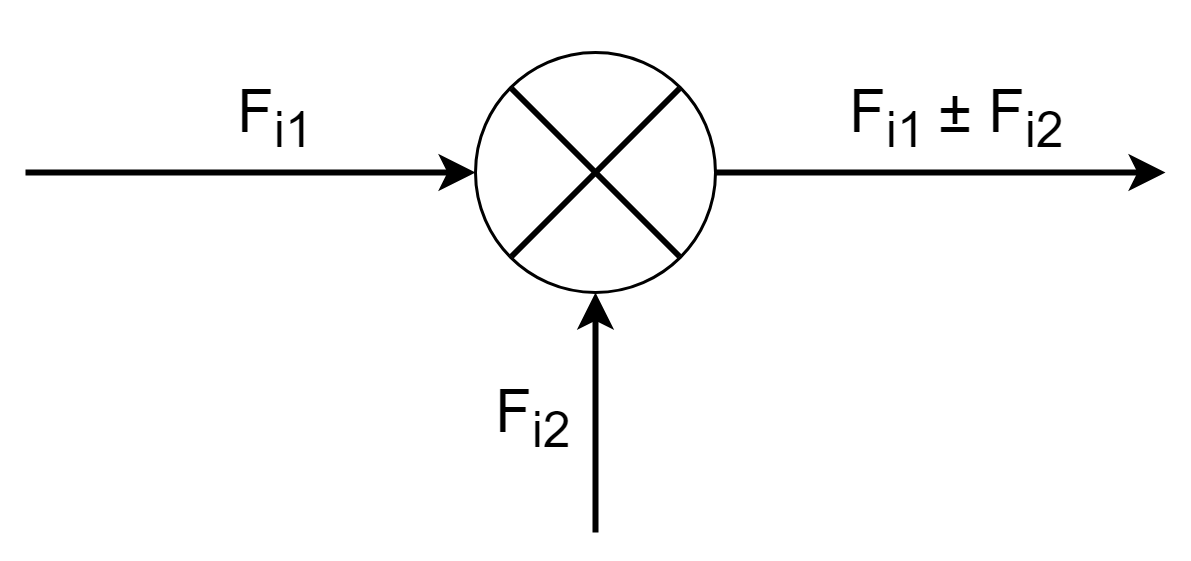
\includegraphics[width=0.8\textwidth]{diag/mixer.png}
    		\caption{\textit{Schematic of RF mixer.}}
		\end{figure}
		
		Where:
		\begin{itemize}
			\item $F_{i1}$ and $F_{i2}$ are input signal that are mixed together.
			\item $F_{i1} + F_{i2}$ is USB (Upper Side Band) output signal,
			\item $F_{i1} - F_{i2}$ is LSB (Lower Side Band) output signal.
		\end{itemize}
		
		In every mixing operation USB and LSB signal are generated. Depending on the relation between $RF$ and $LO$
		signal one of the band is desired output and other is undesired image.
		\\
		
		When $RF$ < $LS$ mixer works as up-converter USB is desired and LSB is undesired.
		\begin{figure}[!htb]
    		\centering
   			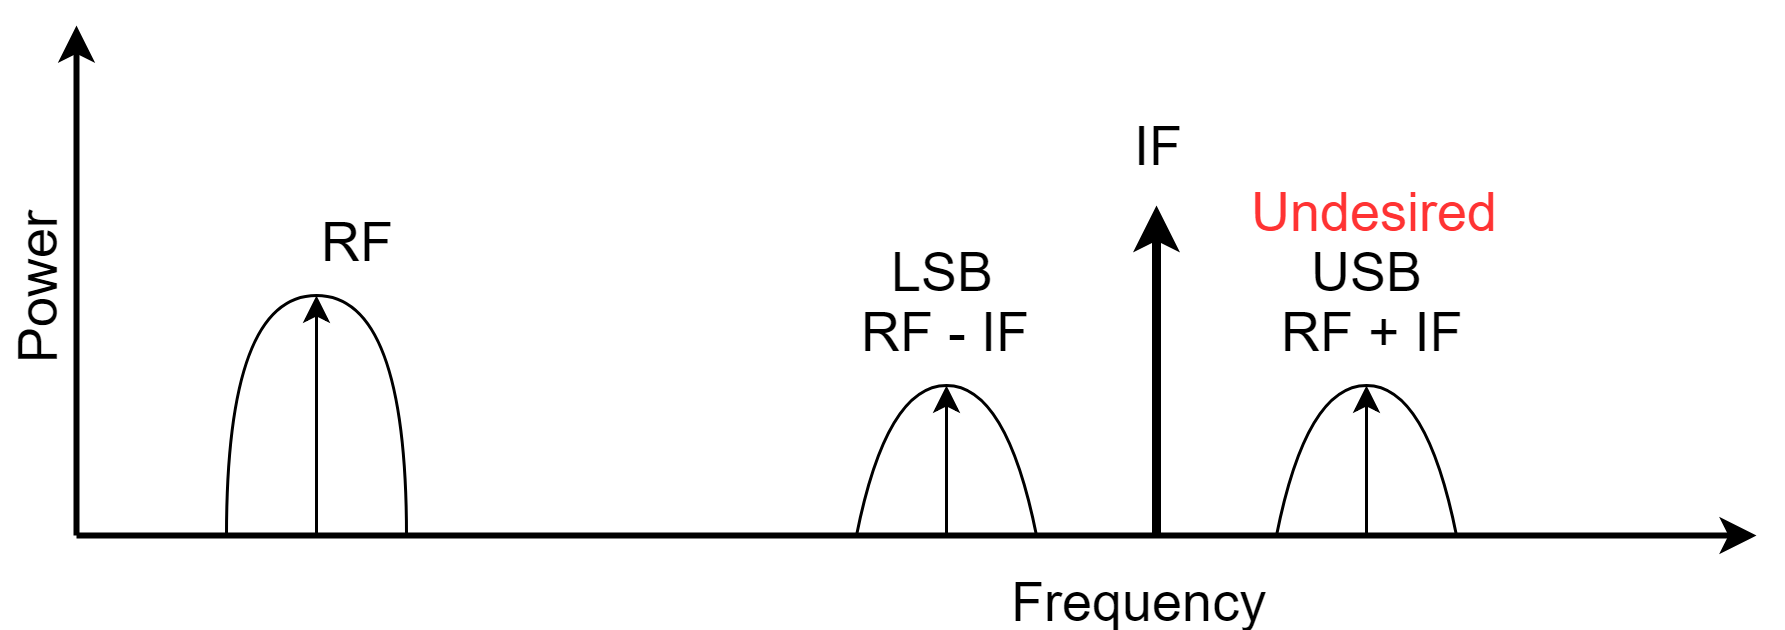
\includegraphics[width=\textwidth]{diag/upconv.png}
    		\caption{\textit{Schematic of RF mixer.}}
		\end{figure}
		
		\begin{figure}[!htb]
    		\centering
   			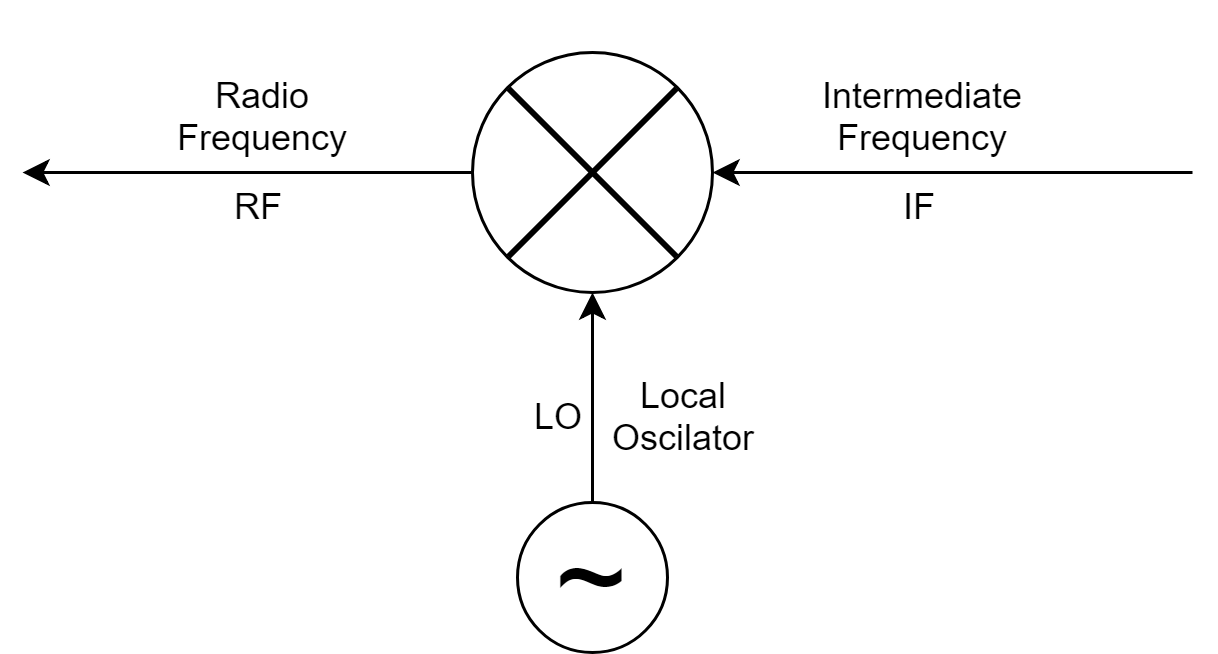
\includegraphics[width=0.6\textwidth]{diag/upmx.png}
    		\caption{\textit{Schematic of RF mixer working as up-converter.}}
		\end{figure}
		
		When $RF$ < $LS$ mixer works as down-converter LSB is desired and USB is undesired..
		\begin{figure}[!htb]
    		\centering
   			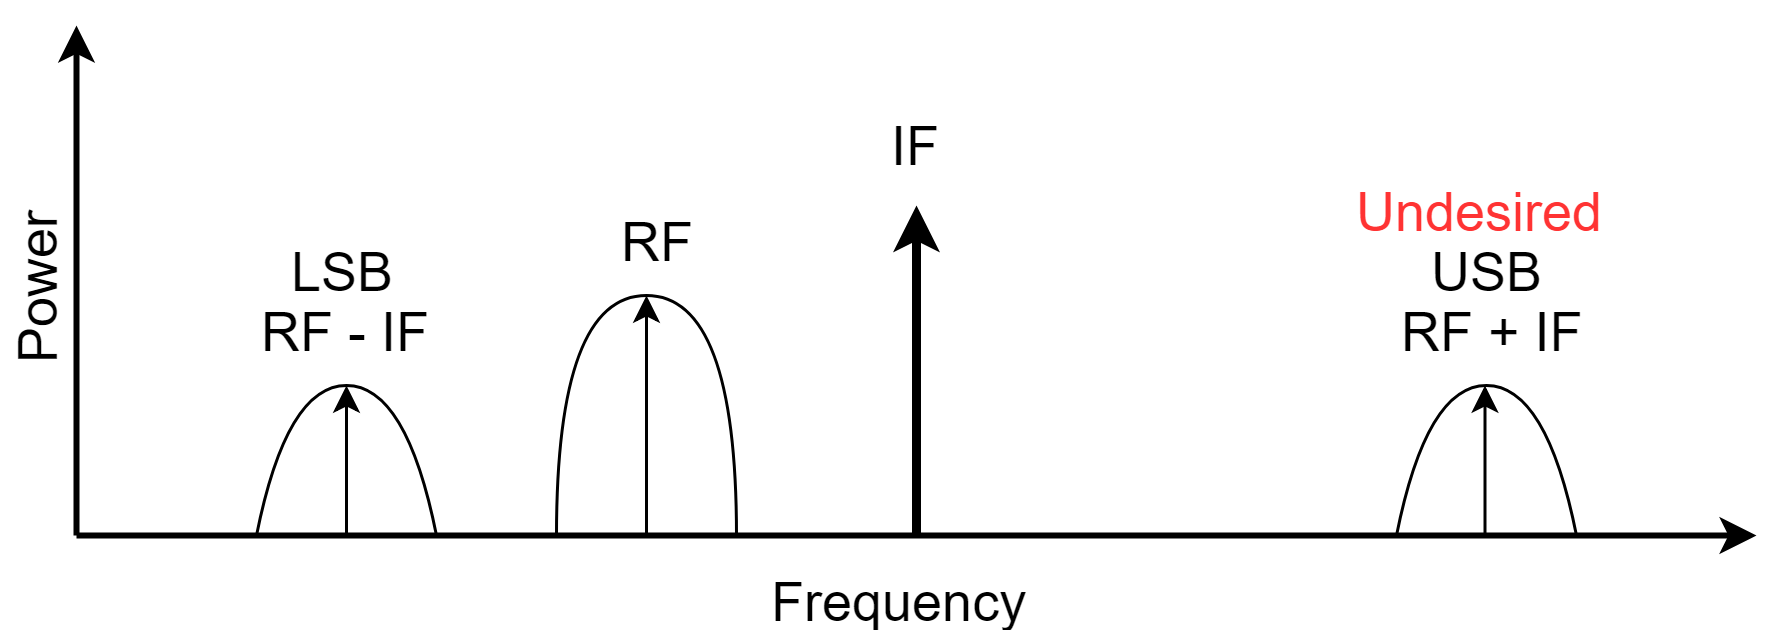
\includegraphics[width=\textwidth]{diag/downconv.png}
    		\caption{\textit{Schematic of RF mixer.}}
		\end{figure}
		
		\begin{figure}[!htb]
    		\centering
   			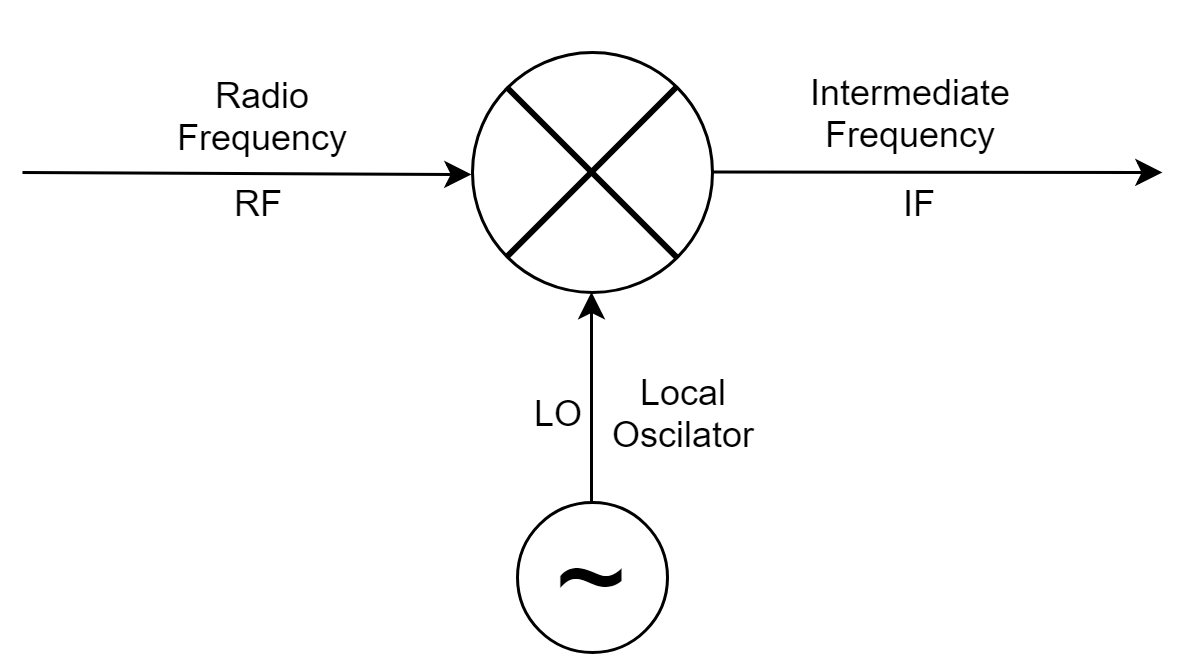
\includegraphics[width=0.6\textwidth]{diag/downmx.png}
    		\caption{\textit{Schematic of RF mixer working as down-converter.}}
		\end{figure}
		
		To remove unwanted band it is necessary to include in the RF mixer design BPFs (Band Pass Filters).
		This filter attenuates all frequencies outside specified band.
		\\
		
		Application for mixers are mostly:
		\begin{itemize}
			\item Frequency shifting - The most common application for RF mixer is changing signal frequency
			with preservation of others parameters such as amplitude and phase.
			This technology is mostly used in RF transmitter and receivers.
			Such devices are called up-converters (for mixing signal with carrier) and down-converter (for
			extracting signal from carrier).
			\item Phase comparison - It is possible to detect phase difference between two signal using mixer.
			This RF mixer application is used in PLLs (Phase Locked Loops).
		\end{itemize}
	
	\section{IQ signal model}
			The term IQ is an abbreviation for in-phase and quadrature. Signal are considered in-phase when phase
		of both is equal and quadrature when it differs by 90$^{\circ}$. IQ data model shows changes in phase and
		magnitude of a sine wave. Modification of these parameters allow to encode information upon a sine wave.
		\\
		
		\noindent				
		Equation of the sine wave is:
		\[
			A cos\left(2\pi f t+ \phi\right), \label{eq:sinewave}
		\]
		where:
		\begin{itemize}
			\item $A$ is amplitude,
			\item $f$ is frequency,
			\item $\phi$ is phase shift
		\end{itemize}
		
		According to equation \label{eq:sinewave} only amplitude, phase and frequency of the sine wave can be
		modified. Moreover frequency is first derivative of phase. Therefore it can be collectively referred to 
		as the phase angle. According to these assumptions the instantaneous state of a sine wave can be described
		in complex plain using magnitude and phase as polar coordinates.
		
		\begin{figure}[!htb]
    		\centering
   			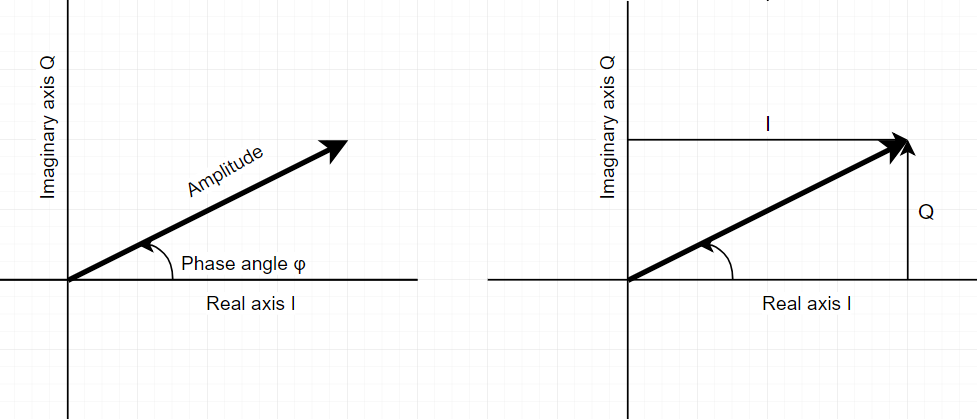
\includegraphics[width=\textwidth]{plots/polarplots.png}
    		\caption{\textit{Representation of sine wave in complex plain}}
    		\label{fig:polarplot}
		\end{figure}
		
		\newpage
		Using trigonometry, the polar coordinates can be converted into I and Q components of the signal using following
		equations:
		\begin{itemize}
			\item $I = A cos\left(2\pi f t\right)$, \label{eq:IQ}
			\item $Q = A sin\left(2\pi f t\right)$,
		\end{itemize}
		\vspace{0.5cm}
		
		IQ data model is widely used in RF communication systems. It gives possibility to distinguish type of 
		modulation used 
		on carrier and allows introduce concept of positive and negative frequency. Amplitude and phase angle form
		seems to be more intuitive, however precisely varying the phase of a high-frequency carrier sine wave in a
		hardware circuit according to an input message signal is difficult. Therefore such hardware modulators will
		be expensive and hard to design and build. To avoid direct modulation of RF signal phase signal is decomposed
		to I and Q components.
		\\
		
		According to Ptolemy’s identitie for the cosine of sum:
		\[
			cos\left(x+y\right) = 
			cos\left(x\right)  cos\left(y\right) - sin\left(x\right) sin\left(y\right)
		\] 
		sine wave carrier can be represented as:
		\[
			Acos\left(2\pi ft + \phi\right) = 
			Acos\left(2\pi ft\right)cos\left(\phi\right) - Asin\left(2\pi\right). ft)sin(\phi)
		\]
		Using equation \ref{eq:IQ} following formula is obtained:
		\[
			Acos\left(2\pi ft + \phi\right) = 
			I cos\left(2\pi f t\right) - Q sin\left(2\pi f t\right),
		\]
		where:
		\begin{itemize}
			\item I - is amplitude of in-phase signal,
			\item Q - is amplitude of quadrature signal.
		\end{itemize}
		
		Using this data samples representation modulation of phase of the RF signal is possible just by modulation of
		I/Q signals amplitudes and then mixing it with carrier and quadrature of carrier using mixers. Schematics below 
		shows structure of IQ modulator and demodulator.
		
		\begin{figure}[!htb]
    		\centering
   			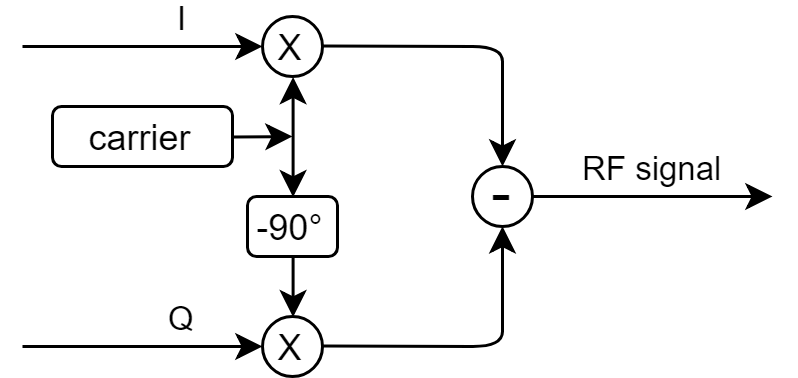
\includegraphics[width=\textwidth]{images/iqmod.png}
    		\caption{\textit{Schematic of IQ modulator}}
    		\label{fig:polarplot}
		\end{figure}
		\vspace{1cm}
		\begin{figure}[!htb]
    		\centering
   			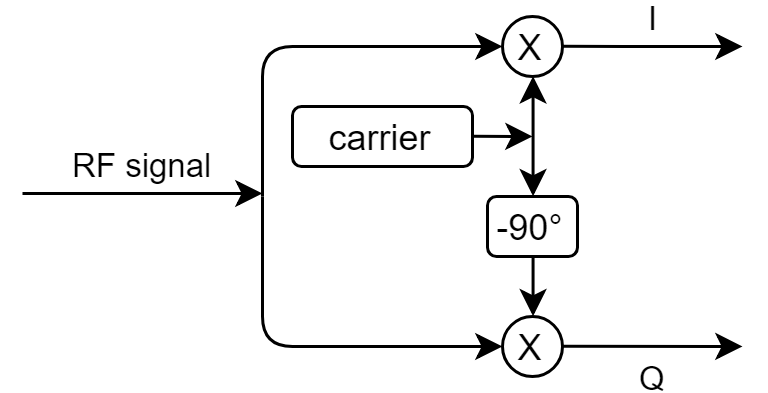
\includegraphics[width=\textwidth]{images/iqdemod.png}
    		\caption{\textit{Schematic of IQ demodulator}}
    		\label{fig:polarplot}
		\end{figure}
		\newpage
		The flexibility and simplicity of this solution compared to direct phase manipulations
		is a reason why I/Q modulators and demodulators are so widely used and popular in RF hardware.
		
	\newpage
	\section{IQ imbalance models}
		In this section two models of IQ mismatch imbalance are presented. First model is called 
		Single-Branch IQ Imbalance Model (SBIQMB) and IQ imbalance is modeled as amplitude and phase
		error in only Q branch. Second is called Double-Branch IQ Imbalance Model (DBIQMB) and 
		models IQ imbalance as amplitude and phase error in both branches.
		
		\subsection*{Single-Branch IQ Imbalance Model}
			This model is characterized by mismatch existing only in Q branch. Amplitude error is
			described as $g$ which results in $1-g$ represents total error in amplitude. Phase mismatch
			is modeled $\phi$. This could be written as equation in following form:
			
		\begin{equation}
			\begin{bmatrix}
				I(t) \\
				Q(t)
			\end{bmatrix}
			=
			\begin{bmatrix}
				1 & 0 \\
				-g sin(\phi) & g cos(\phi)
			\end{bmatrix}
			\begin{bmatrix}
				I_{RF}(t) \\
				Q_{RF}(t)
			\end{bmatrix} \label{eq:SBIQIM}
		\end{equation}
		
		\begin{figure}[!htb]
    		\centering
   			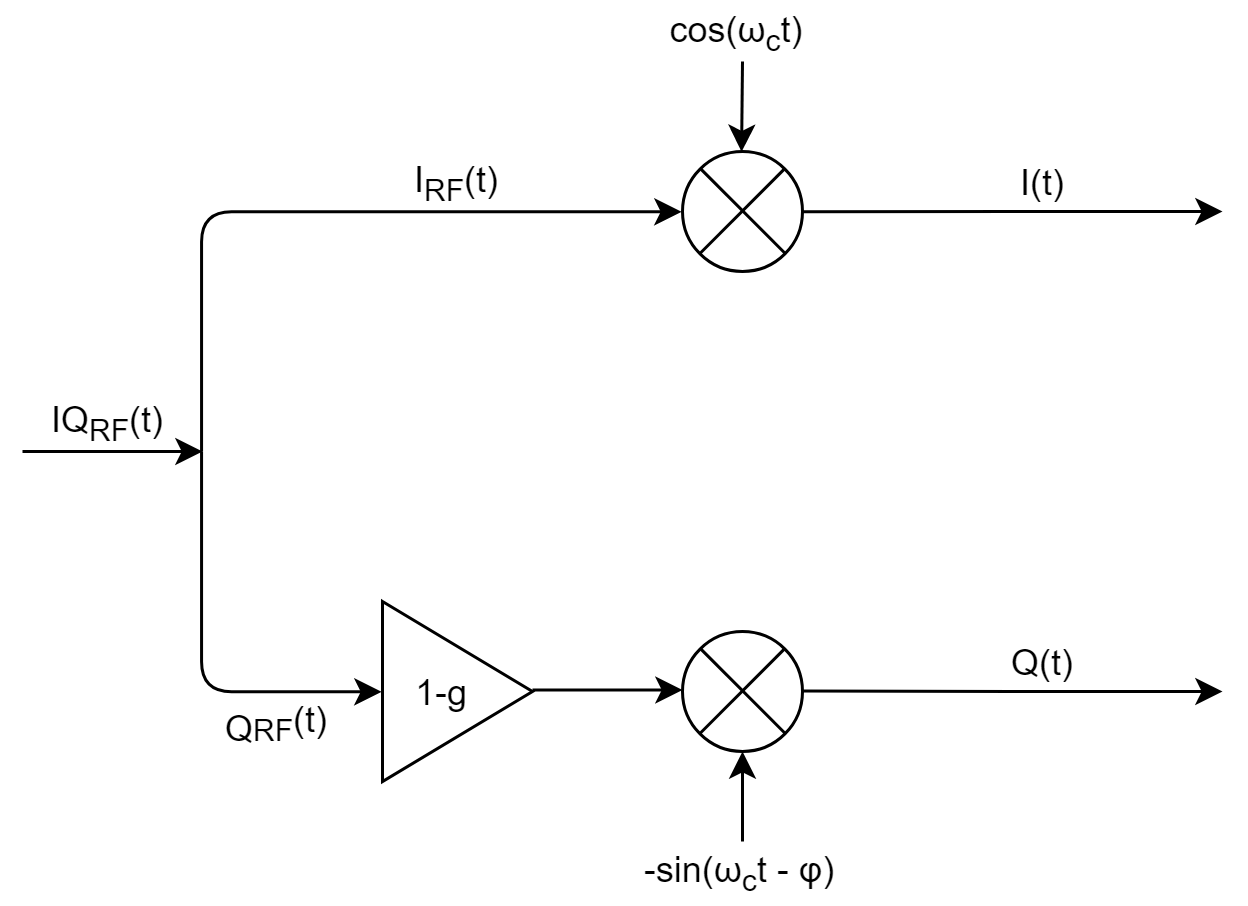
\includegraphics[width=\textwidth]{diag/sbiq.png}
    		\caption{\textit{Schematic of SBIQIM.}}
		\end{figure}
		
		where:
		\begin{itemize}
			\item $I_{RF}(t)$ and $Q_{RF}(t)$ IQ components of received signal.
			\item $I(t)$ and $Q(t)$ IQ components with introduced mismatch.
		\end{itemize}
		\subsection*{Double-Branch IQ Imbalance Model}
			This model is characterized by mismatch existing in Q both. In the I branch 
			mismatch is described as amplitude error 1 + $\epsilon$ and phase error $\phi$.
			Respectively in Q branch amplitude error is 1 - $\epsilon$ and phase 
			error is $-\phi$.
			
			\vspace{1cm}
			\begin{equation}
				\begin{bmatrix}
					I(t) \\
					Q(t)
				\end{bmatrix}
				=
				\begin{bmatrix}
					(1 + \epsilon) cos(\phi) & (1 + \epsilon) sin(\phi) \\
					(1 - \epsilon) sin(\phi) & (1 - \epsilon) cos(\phi)
				\end{bmatrix}
				\begin{bmatrix}
					I_{RF}(t) \\
					Q_{RF}(t) 
				\end{bmatrix} \label{eq:DBIQIM}
			\end{equation}
			\vspace{0.5cm}
			\begin{figure}[H]
    		\centering
   				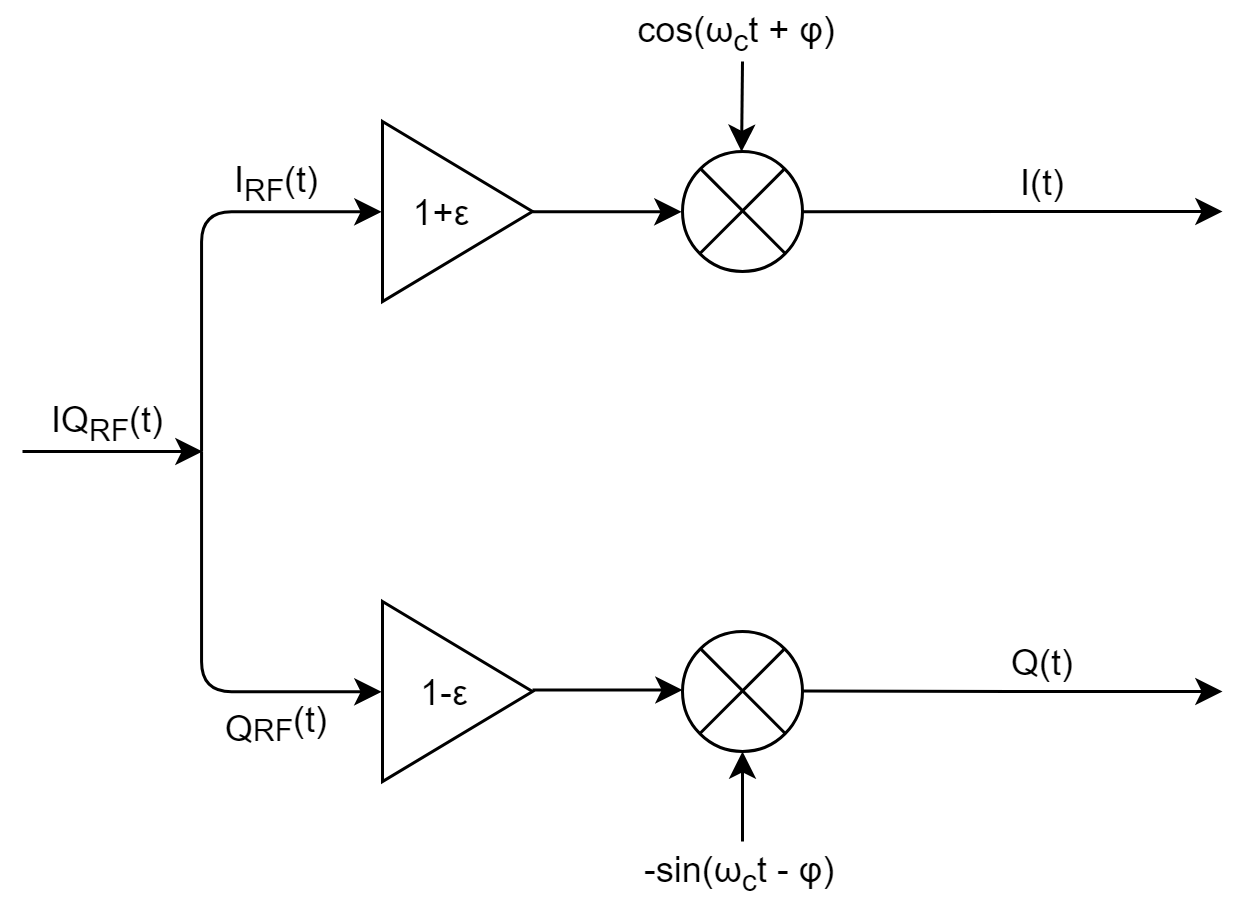
\includegraphics[width=\textwidth]{diag/dbiqm.png}
    			\caption{\textit{Schematic of DBIQIM.}}
			\end{figure}
			
		where:
		\begin{itemize}
			\item $I_{RF}(t)$ and $Q_{RF}(t)$ IQ components of received signal.
			\item $I(t)$ and $Q(t)$ IQ components with introduced mismatch.
		\end{itemize}
		\newpage
		\subsection*{Relation between SBIQIM and DBIQIM}
			As mentioned before both models describes IQ mismatch in different ways. DBIQIM is
			equivalent to SBIQIM processed by two additional matrices. Matrix $G$ that represents gain
			and matrix $R$ which represents rotation.
			Equations below shows relation between SBIQIM and DBIQIM:
			\\
			
			
			As mentioned earlier:
			\[
				SBIQIM = 
				\begin{bmatrix}
				1 & 0 \\
				-g sin(\phi) & g cos(\phi)
				\end{bmatrix}
			\]
			\[
				DBIQIM = 
				\begin{bmatrix}
					(1 + \epsilon) cos(\phi) & (1 + \epsilon) sin(\phi) \\
					(1 - \epsilon) sin(\phi) & (1 - \epsilon) cos(\phi)
				\end{bmatrix}
			\]
			\vspace{0.5cm}
			\begin{equation}
				DBIQM = G\cdot SBIQIM \cdot R
			\end{equation}
			\\
			
			
			$G$ and $R$ are defined as follows:
			\begin{equation}
				G = \frac{2}{1+g}
			\end{equation}
			\begin{equation}
				R = 
				\begin{bmatrix}
					cos(-\frac{\phi}{2}) & sin(-\frac{\phi}{2}) \\
				   -sin(-\frac{\phi}{2}) & cos(-\frac{\phi}{2})
				\end{bmatrix}
			\end{equation}
			\\
			
			
			Using equation above transition between models parameters works as follows:
			\begin{itemize}
				\item Calculation of DBIQIM parameters based on SBIQIM.
				\[
					\epsilon = \frac{1-g}{1+g}
				\]
				\[
					\phi_{DBIQIM} = - \phi_{SBIQIM}/2
				\]
				\item Calculation of SBIQIM parameters based on DBIQIM.
				\[
					g = \frac{1-\epsilon}{1+\epsilon}
				\]
				\[
					\phi_{SBIQIM} = - 2\phi_{DBIQIM}
				\]
			\end{itemize}
			
	\newpage
	\section{Software Defined Radio}
		SDR (Software Defined Radio) is a radio communication system where components typically
		 implemented in hardware 
		(e.g. mixers, filters, amplifiers, modulators/demodulators), are instead implemented
		 by the means of software.
		\\
		
		
		Below the block diagram of SDR device is presented:
		\begin{figure}[!htb]
    		\centering
   			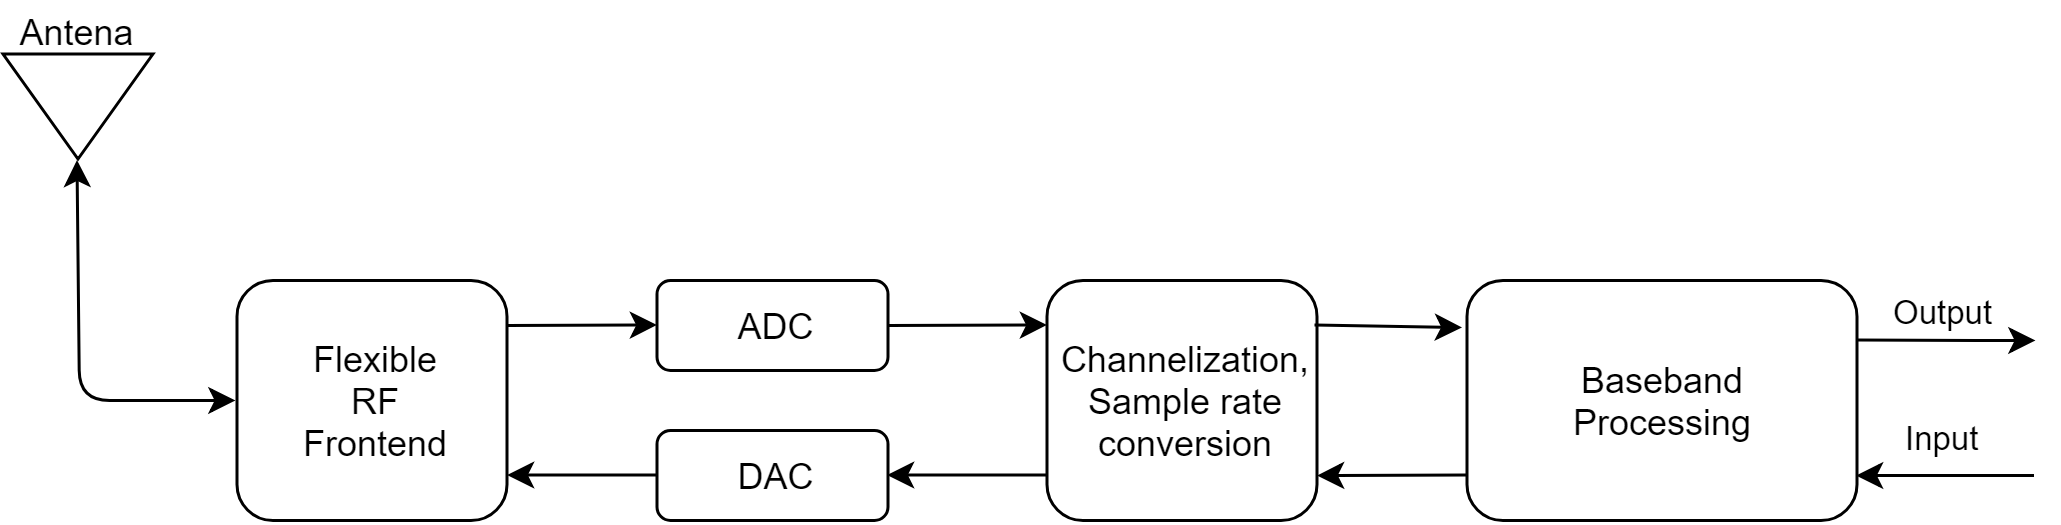
\includegraphics[width=\textwidth]{diag/sdr.png}
    		\caption{\textit{Block diagram of SDR device.}}
		\end{figure}
		
		\begin{itemize}
			\item \textbf{Flexible RF fronted} is a first stage of SDR processing system. This part is configured by the means
			software to match current requirements for best system performance. This is possible by using numerically
			controlled components.
			NCO (Numerically Controled Oscilators) which are used as flexible frequency generators. This component are
			essential for I/Q modulators/demodulators as flexible carrier generators for mixers. Bandpass filters and equalizers\
			used for signal conditioning.
			
			\item \textbf{ADC / DAC converters}. This is where captured signal is converted from analog to digital domain and
			likewise transmited is converted form digital to analog domain. This is a last stage before before purely digital 
			domain of the system.
			
			\item \textbf{Channelization and Sample rate conversion}. Here the data processed by the baseband system are assigned
			to respective communication channels, and conditioned for specific channel transmission parameters like frequency and
			sampling rate.
			
			\item \textbf{Baseband Processing System} Digital core of the SDR system. This may by either processor, FPGA, ASIC or
			SoC. Variety of choice in this case allows creation of well-suited system for desired performance and cost range. 
			Mentioned component is responsible with interfacing with external system for data exchange purpose. All logic related to
			transmission is implemented here in the software including correction algorithms and application layer. Thanks to that
			system can adapt to changes. This means changing software to improve quality of the processed signal
			or even complete change of the application layer, by simply providing new software.
		\end{itemize}
		
		SDR devices are characterized by very fast ADC and DAC converters which are necessary for 
		direct conversion. For example in secondary air plain surveillance systems (ADS-B), the
	    carrier frequency is 1.09GHz. By Nyquist law this requires at least two times higher frequency
	    sampling which is 2.18GHz.
	    
\chapter{Hardware and tools}
	This chapter describes chosen hardware, tools and explains reasons behind such decisions.
	\section{Adalm Pluto and AD tools}
		\subsection*{Adalm Pluto Board}
			Adalm Pluto is learning module from Analog Devices that can be used to introduce 
			principles of operation and theory behind SDR and RF communication.
			
			\begin{figure}[!htb]
    			\centering
   				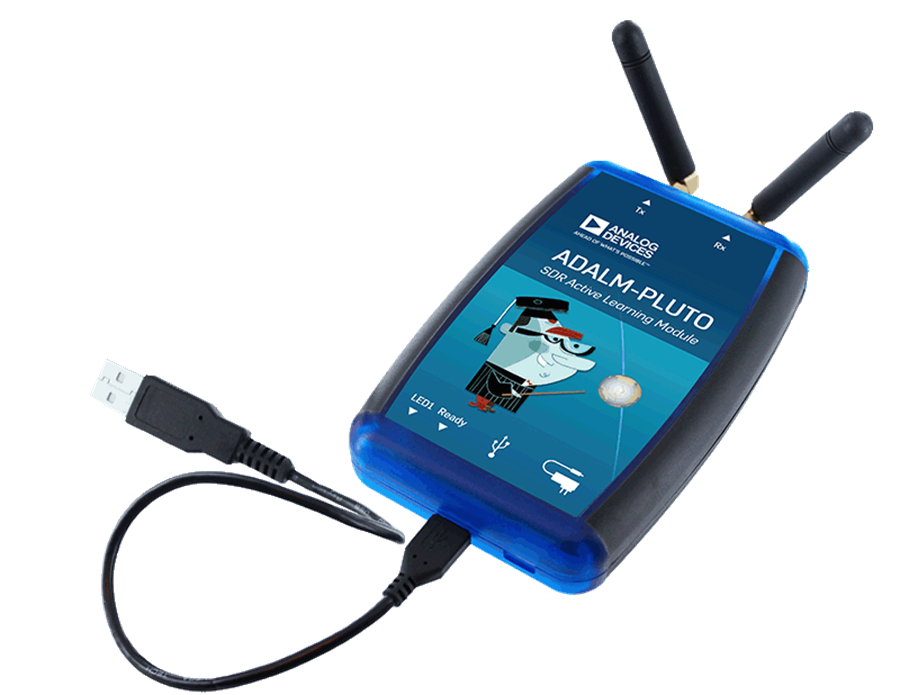
\includegraphics[width=\textwidth]{images/plutoimg.png}
    			\caption{\textit{Photo of Adalm Pluto device \cite{pluto_photo}.}}
			\end{figure}
			\newpage
			\begin{figure}[!htb]
    			\centering
   				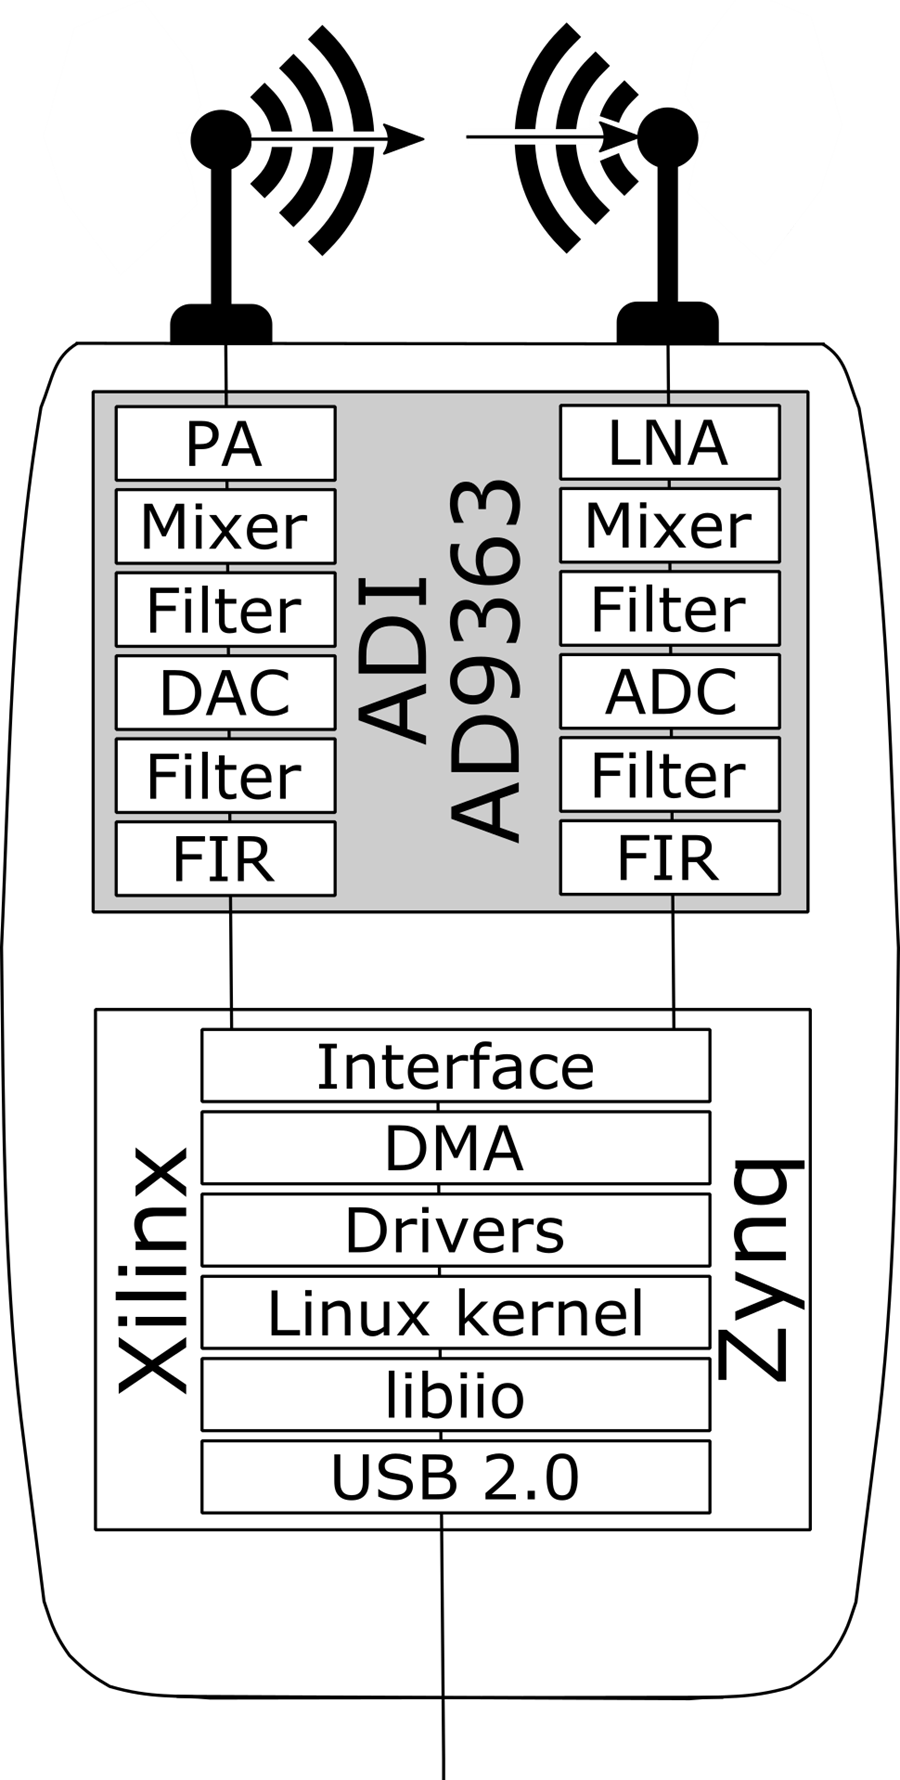
\includegraphics[width=11cm]{images/pluto_schematic.png}
   		 		\caption{\textit{Schematic Adalm Pluto hardware \cite{pluto_scheamtic}.}}
			\end{figure}
			
			Adalm Pluto is already integrated with with MATLAB, Simulink, GNU Radio, and libIIO which
			allows to interface with the devices using C, C++, C\# or Python programming languages.
			PlutoSDR is open software repository with all software and tools related to Adalm Pluto
			including: HDL Project in Xillinx Vivado and Buildroot configuration for embedded Linux.
			Main reason for choosing this SDR device was relatively low price 136.80USD 
			in comparative to other
			available solutions on the market. Adalm Pluto core is 			
			Zynq7010 SoC which is combination of ARM based processor capable of running Linux and
			FPGA part which can communicate with the processor via AXI interface.
		\subsection*{AD9363 Agile RF Transceiver}
			The main part of Adalm Pluto SDR is AD9363.  AD9363 is a high performance, highly
			integrated RF agile transceiver designed for use in 3G and 4G femtocell applications.
			
			\begin{figure}[!htb]
    			\centering
   				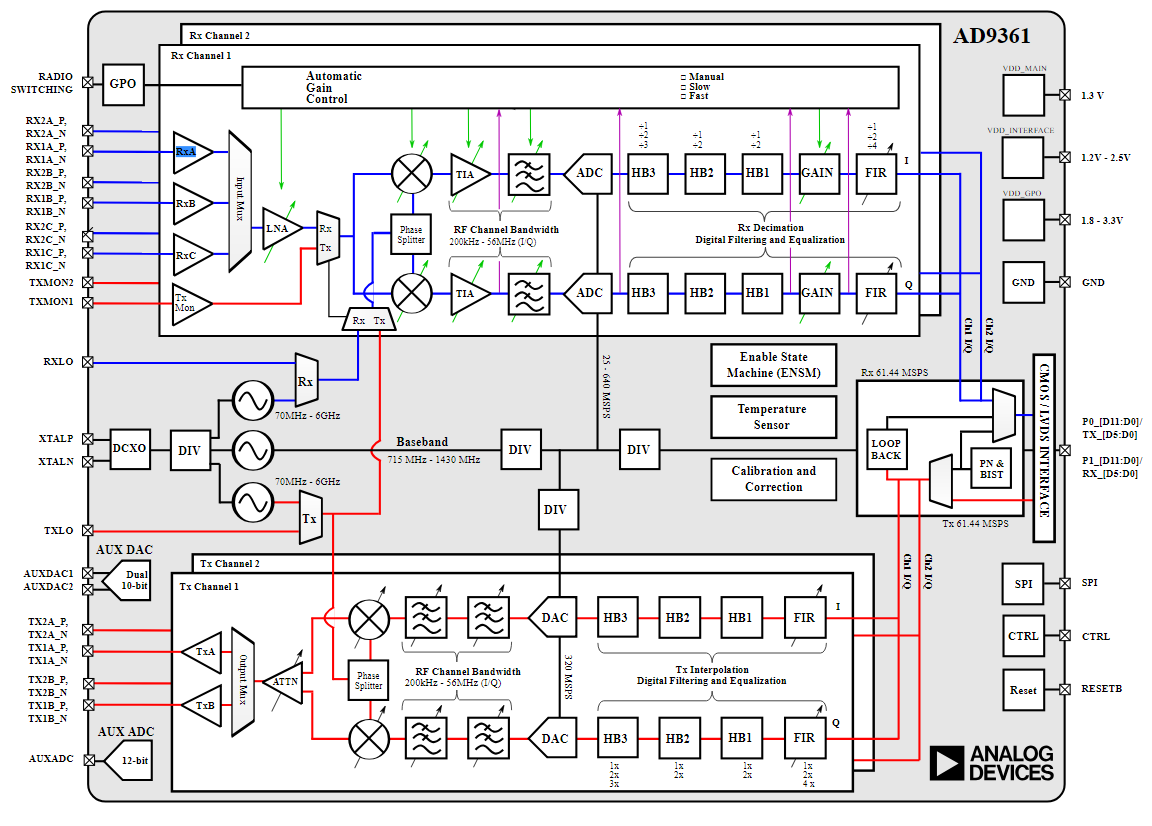
\includegraphics[width=\textwidth]{images/ad9361_sch.png}
   		 		\caption{\textit{Block diagram of AD9363 RF transceiver \cite{ad9363_diag}.}}
			\end{figure}
			
			Ad9363 features:
			\begin{itemize}
				\item Wide bandwidth from 325Mhz to 3.8GHz,
				\item Tunnable channel bandwidth up to 20MHz,
				\item Independent AGC (Automatic Gain Control),
				\item Full duplex communication,
				\item DC offset and I/Q mismatch tracking.
				\item Flexible rate, 12-bit ADC and DAC
			\end{itemize}
		\subsection*{IIO Osciloscope}
			The ADI IIO Oscilloscope is application which allows interfacing with different
			evaluation or custom made board based on AD agile RF Transrecivers. This program allows
			communication with the device connected with PC
			using:
			\begin{itemize}
				\item Local or remote network,
				\item USB 2.0 interface,
				\item Serial Port.
			\end{itemize}			 
			
			Application supports full configuration of the device including: configuration receiver
			frequency and channel bandwidth. Access to DC offset tracking, I/Q correction,
			internal calibration functionality and all registers. Moreover allows to process revived
			using filters designed in matlab and four gain control modes:
			\begin{itemize}
				\item manual configuration - gain is selected by user,
				\item slow attack approach,
				\item fast attack approach,
				\item hybrid attack approach,
				
			\end{itemize}
			\vspace{5mm}
							
			\noindent
			Program allows to plot received data from selected channels in four different modes:
			\begin{itemize}
				\item time domain as I and Q signals,
				\item frequency domain with configurable FFT and averaging size,
				\item constellation as relation between I and Q signals,
				\item cross-correlation for multi-channel boards.
			\end{itemize}
			
	\section{libIIO}
		libIIO is library developed by Analog devices for interfacing Linux IIO (Industrial
		Input Output) devices.
		
		Library is composed of three main parts:
		\begin{itemize}
			\item local backend - responsible for  interfacing with the Linux kernel using
				sysfs virtual file system,
			\item network backend - which communicates with the IIOD (IIO Deamon) by network link.	
		\end{itemize}
		
		The IIOD is libiio based application that creates libiio context which is using local backend
		and then connects it to network backend. Described process allows to share local context
		with the server and makes device accessible via network

		
		\begin{figure}[!htb]
    		\centering
   			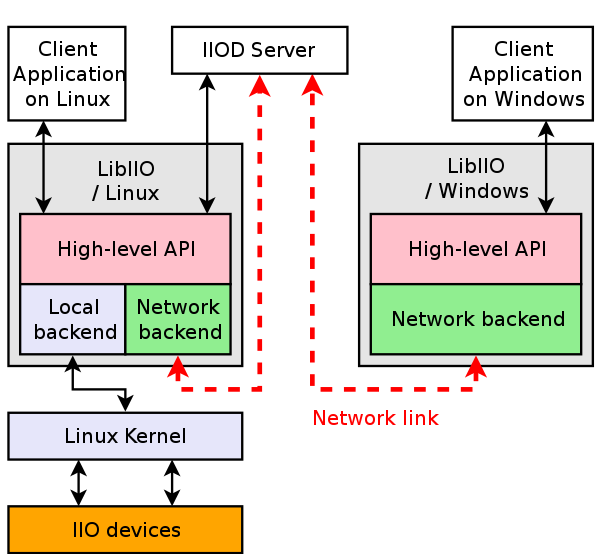
\includegraphics[width=\textwidth]{images/libiio_diagram.png}
   		 	\caption{\textit{Block diagram of libIIO working principles. \cite{libioo}}}
		\end{figure}
		
		\newpage
	\section{Zynq and Xilinx tools}
		\subsection*{Introduction to SoC}
		SoC is aberration from System on Chip. Such devices aggregates
		many types of hardware in single chips including: ADCs, DACs, internal memory, external 
		memory controllers, peripheral interfaces such as SPI, UART, I2C and many others. 
		The main idea is that single silicon chip may be
		used to implement functionality of entire system. Such approach results in cheaper and faster solution than
		realizing such functionality on PCB using separate components. In the past such role
		belonged to ASIC.
		(Application Specific Integrated Circuits). The major disadvantages of such solution is lack
		of flexibility and significant development cost and time. This makes ASIC's sustainable only
		on the high volume market where no future upgrade will be required. These limitations created
		clear need for more flexible device with faster development time. This need has been long
		satisfied by a FPGAs. FPGA can be reconfigured as desired which means virtually no risk in
		deploying solution which may require upgrade based on FPGA. Next step are SoC based solution.
		SoC is combination of processor and FPGA. This allows to create fast application dependent on the
		hardware functionality. Moreover processor can run normal operating system which allows fast
		development and flexibility of the solution.
		
		\subsection*{Zynq-7000 family SoC}
		The Zynq is new kind of SoC from Xillinx. It combines both applications processor and FPGA 	
		fabric. The Zynq device comprises two sections: PS (Processing System) and PL (Programmable
		Logic). This sections can be used separately for independent task or together to utilize
		advantages of both software and hardware. The Zynq devices are meant to use structure of
		both sections and interface between them. Connection between these parts is provided by AXI
		(Advanced eXtensible Interface) which is registered under ARM trademark.
		\\
		
		Processing System in all Zynq devices has the same architecture, and the base of it is
		a dual-core ARM Cortex-A9 processor. This is a hard processor which means it is manufactured
		directly in silicon structure. Zynq allows to use soft processors like PicoBlaze and 
		MicroBlaze which can be implemented in PL sections. Depending on the size and speedgrade of
		the device ARM processor is accompanied by set of processing resources e.g (MMU, DMA, SRAM,
		Processing System External Interfaces, cache memory, control registers , etc.) which forms
		together APU (Application Processing Unit).
		
		\begin{figure}[!htb]
    		\centering
   			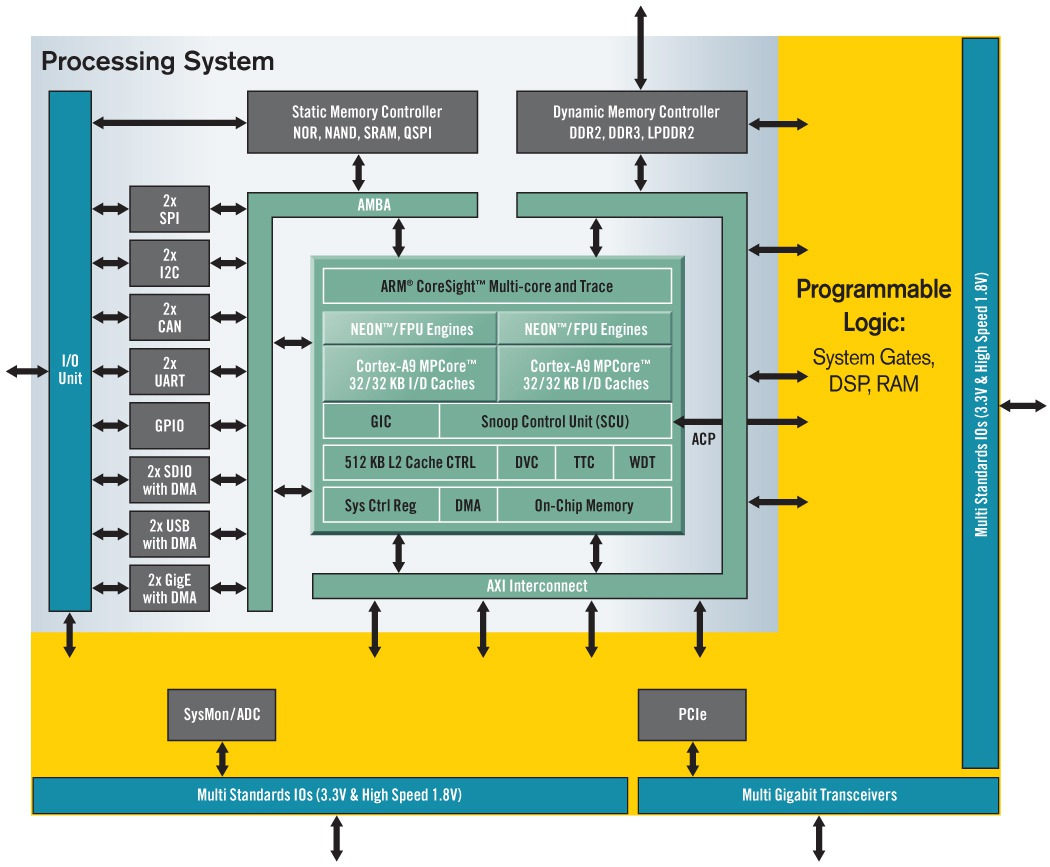
\includegraphics[width=\textwidth]{images/zynq.jpeg}
   		 	\caption{\textit{Block diagram fo Zynq 7000 family SoC. \cite{zynq_diag}}}
		\end{figure}
		\newpage

		Programmable Logic is a FPGA based on Atrix-7 and Kintex-7 fabric from Xillinx. PL consist of
		CLBs ( Configurable Logic Blocks ), slices, IOBs( Input Output Blocks), LUTs (Lookup tables),
		fliplops and switch matrices. Additionally there are BRAM (Block Random Access Memory) which
		are used to store large amout of date in small part of the device which allows fast access to
		its content. Second additional resource is DSP48E1 slice. This is advanced DSP module that
		allows many complex mathematical operation in a single clock cycle.
		
		\subsection*{Xillinx Vivado Tools}
			As a part of Zynq-7000 family SoC design flow. Xillinx Vivado 2018.2 and Xilinx Vivado HLS
			2018.2 where choosen. This version of the software is tested and compatible with latest
			release of the plutosdr-fw repository.
			\\
			
			Xillinx Vivado is a tool for FPGA design. This program allows full configuration of
			PL part of the Zynq-7000 family SoC including: synthesis, implementation, routing,
			timing validation and generation of the bitstream. Bitstream is used to deploy configuration
			onto FPGA device.
			
			Xilinx Vivado HLS is a program for High Level Synthesis for Zynq-7000 family SoC. This 
			tool allows to write and test software in C language. After proper validation in the software
			domain, code can be synthesized to HDL and exported to Xillinx Vivado as an IP Core.
			This allows much faster design than direct HDL development and much easier testing.
			These were main reason for choosing HLS environment.
	
\chapter{Algorithms}
	This chapter describes all algorithms used for signal quality improvement. All of considered 
	algorithms are blind. This means that signal analysis is purely statistical with no prior 
	information about signal. Advantages of this approach is that this algorithms can be used 
	for any type of possible signal.
	\section{DC offset correction}
		This section describes algorithms used for removing DC offset from revived samples.
		\subsection*{Moving Average Filter}
			Moving Average Filter is simple FIR (Finite Impulse Response) filter. This filter is
			commonly used for white noise removal and signal smoothing. However when filter order
			is great enough to account for samples from full period of the signal filters the
			average represents signal DC offset.
			\\
			
			
			The filter equations is presented below \cite{mav}:
			\begin{equation}
				y[n] = \frac{1}{N} \sum_{k=0}^{N-1}x[n-k], \label{eq:mva_fir} 
			\end{equation}
			
			where:
			\begin{itemize}
				\item   $N$ is order of the filter.
				\item	$y[n]$ is filtered sample at n-th step,
				\item   $x[n]$ is n-th sample from receiver.
			\end{itemize}			
			
			DC components of I and Q branches are calculated using equation \ref{eq:mva_fir},
			where $x[n-k]$ is substituted with corresponding I or Q sample.

			\[
				I_{mean}[n] = \frac{1}{N} \sum_{k=0}^{N-1}I[n-k]
			\]
			\[
				Q_{mean}[n] = \frac{1}{N} \sum_{k=0}^{N-1}Q[n-k]
			\]
			
			Corrected values are calculated as follows:
			\[
			\renewcommand*{\arraystretch}{1.3} 
			\begin{array}{ll}
				I_{corr}(n) = I(n) - I_{mean}(n), \\
				I_{corr}(n) = Q(n) - Q_{mean}(n)
			\end{array}
			\]
			
			Algorithm introduces delay by N samples in the signal. It is important to that the number of
			samples taken into consideration must extend at least one period of the signal. Otherwise
			filter will works white noise attenuator.
			
		\subsection*{Normalized Gaussian Filter}
			Normalized Gaussian Filter is filter whose impulse response has shape of Gaussian
			function with all values in range from 0 to 1.
			
			\[
				G(x) = \frac{1}{ \sqrt{2\pi \sigma^2}}e^{\frac{-x}{2\sigma^2}}
			\]
			where:
			\begin{itemize}
				\item $x$ is 
				\item $\sigma$ is standard deviation. 
			\end{itemize}
			
			The filter equations is presented below \cite{filter_design}
			\begin{equation}
				y[n] = \sum_{k=0}^{N-1}x[n-k]G(x) \label{eq:gauss}
			\end{equation}
			\begin{itemize}
				\item N is windows size,
			\end{itemize}	
			DC components of I and Q branches are calculated using equation \ref{eq:gauss},
			where $x[n-k]$ is substituted with corresponding I or Q sample.
			\[
				I_{mean}[n] = \sum_{k=0}^{N-1}x[n-k]G(x)
			\]
			\[
				Q_{mean}[n] = \sum_{k=0}^{N-1}x[n-k]G(x)
			\]		
			Corrected values are calculated as follows:
			\[
			\renewcommand*{\arraystretch}{1.3} 
			\begin{array}{ll}
				I_{corr}(n) = I(n) - I_{mean}(n), \\
				I_{corr}(n) = Q(n) - Q_{mean}(n)
			\end{array}
			\]
			This filter has better performance in frequency domain than Moving Average Filter.
			
	\section{IQ Mismatch Correction}
		The IQ imbalance is common problem in RF front-ends that uses analog quadrature down-
		mixing. The ideal down-converter performs only simple frequency shift. Real down-
	    converters introduces image interference which may be assumed as constant. But amplifiers
	    and filters introduces varying with frequency imbalance.
	    
	    In ideal case the receiver output is:
		\begin{equation}
			\renewcommand*{\arraystretch}{1.3} 
			\begin{array}{ll}
				I(t) = cos(\omega t) \\
				Q(t) = sin(\omega t) \\
			\end{array}
		\end{equation}
		where:
		\begin{itemize}
			\item $\omega$ is tone frequency.
		\end{itemize}
	    I and Q components are orthogonal with respect to each other.
	    In real case receiver output is:
		\begin{equation}
			\renewcommand*{\arraystretch}{1.3} 
			\begin{array}{ll}
				I(t)' = \alpha cos(\omega t) + \beta_I \\
				Q(t)' = sin(\omega t + \phi) + \beta_Q \\
			\end{array}
		\end{equation}
		where:
		\begin{itemize}
			\item $\alpha$ is magnitude mismatch,
			\item $\phi$ is phase imbalance,
			\item $\beta_{IQ}$, $\beta_{Q}$ is signal DC offset.
		\end{itemize}
		Input of phase correction algorithms is signal with DC offset extracted using algortihms
		from previews section. Hence the signal model is \cite{iqcorr}
		\begin{equation}
			\renewcommand*{\arraystretch}{1.3} 
			\begin{array}{ll}
				I(t)'' = \alpha cos(\omega t) \\
				Q(t)'' = sin(\omega t + \phi) \\
			\end{array} \label{eq:iqreal}
		\end{equation}
		According to Ptolemy’s identitie for the sine of sum:
		\[
			sin\left(\omega t + \phi\right) = 
			sin\left(\omega t\right))cos\left(\phi \right) + 
			cos\left(\omega t\right) sin\left(\phi \right)
		\] 
		Equation \ref{eq:iqreal} be rewritten in matrix form as:
		\begin{equation}
			\begin{bmatrix}
				I(t)'' \\
				Q(t)''
			\end{bmatrix}
			=
			\begin{bmatrix}
				\alpha & 0 \\
				sin(\phi) & cos(\phi)
			\end{bmatrix}
			\begin{bmatrix}
				I(t) \\
				Q(t)
			\end{bmatrix} \label{eq:iqrealmat}
		\end{equation}
		After multiplying both sides of \ref{eq:iqreal} by inversion of parameters matrix following set of exuations
		is obtained:
		\begin{equation}
			\begin{bmatrix}
				I(t) \\
				Q(t)
			\end{bmatrix}
			=
			\begin{bmatrix}
				\alpha^{-1} & 0 \\
				\alpha^{-1}tan(\phi) & sec(\phi)
			\end{bmatrix}
			\begin{bmatrix}
				I''(t) \\
				Q''(t)
			\end{bmatrix}
		\end{equation}
		This shows that only $\alpha$ and $\phi$ must be found to perform I/Q mismatch
		compensation. According to this paper:
		\[
			<I''(t)I''(t)> = \frac{1}{2}\alpha^2
		\]
		\[
			\alpha = \sqrt{2<I''(t)I''(t)>}
		\]
		\[
			<I''(t)Q''(t)> = \frac{1}{2}\alpha^2sin(\phi)
		\]
		\[
			sin(\phi)= \frac{2}{\alpha}<I''(t)Q''(t)>
		\]
		Assuming that $|\phi| \leq \frac{pi}{4}$ $cos(\phi)$ can be obtained directly from
		$\sin(\phi)$ using following formula:
		\[
		 	cos(\phi) = \sqrt{1-sin(\phi)}
		\]
		Using following parameters in we can substitute matrix equations \ref{eq:iqrealmat} with:
		\begin{equation}
			\begin{bmatrix} 
				I(t) \\
				Q(t)
			\end{bmatrix}
			=
			\begin{bmatrix}
				\frac{1}{\alpha} & 0 \\
				\frac{-sin(\phi)}{acos(\phi)} & \frac{1}{cos(\phi)}
			\end{bmatrix}
			\begin{bmatrix}
				I''(t) \\
				Q''(t)
			\end{bmatrix}\label{eq:iqcorr}
		\end{equation}
		The IQ mismatch correction  can be now applied using \ref{eq:iqcorr} formula.
	
\chapter{Hardware Implementation}
	This chapter explains structure of hardware implemented in Zynq PL section. This includes data flow
	from PS to AD9361 RF transceiver, including correction algorithms for RF signal quality improvement.
	
	\section{Data Flow Path}
	Diagram below shows data path for I/Q samples from Zynq PS system to PL logic.
	
	\begin{itemize}
		\item \textit{AXI_AD9361} - IP core provided by Analog devices. This block is responsible for
			interfacing with AD9363 RF transceiver placed on board. 
		\item \textit{FIR Decimator} - down-sampling block with additional filters to block unwanted
			images created by change of sampling frequency in receive path.
		\item \textit{FIR Interolator} - up-sampling block with additional filters to block unwanted
			images created by change of sampling frequency in transmit path.
		\item \textit{DC Offset Removal} - implementation of dc offset removal algorithm. 
			Depending on test bench Moving Average or Gaussian Filter.
		\item \textit{I/Q Correction} - realization of phase and magnitude correction in the revived
		 	signal.
		\item \textit{Zynq Processing System} - CPU part of Zynq SoC. Mentioned block is responsible for
			communication between PL and PS part using AXI interface. Zynq PS section perform task
			related to data aquisition and interfacing with PC using USB 2.0 interface.
	\end{itemize}
	
	\begin{figure}[H]
    	\centering
   		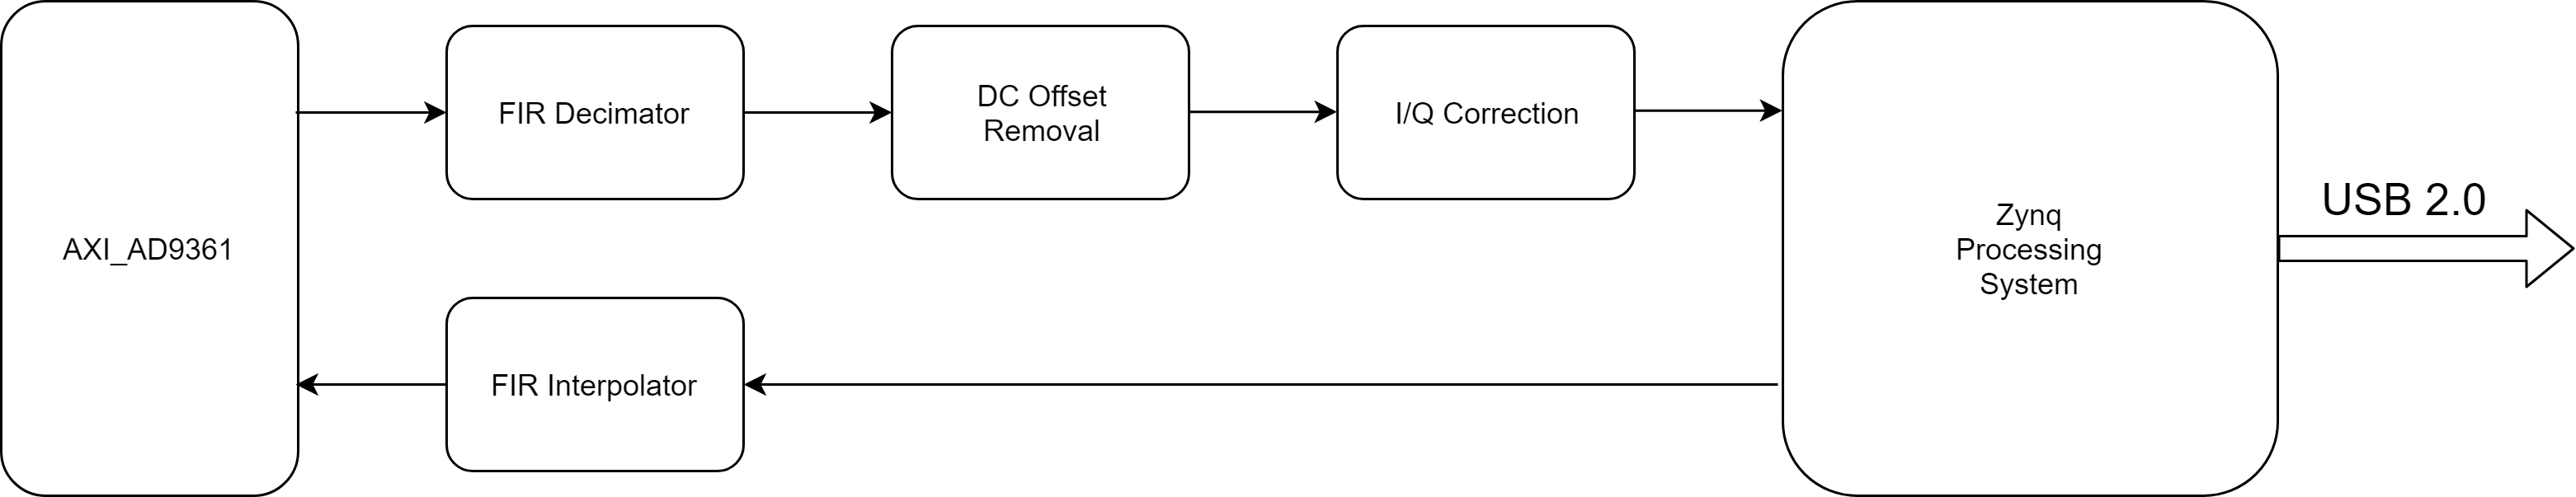
\includegraphics[width=\textheight, angle =90]{diag/hdl.png}
    	\caption{\textit{Block diagram of the PS logic structure.}}
    	\label{fig:polarplot}
	\end{figure}
	
	\section{Moving Average Filter}
	\begin{table}[H]
		\centering
		\caption{}
		\begin{tabular}{|c|c|c|c|}
		\hline
		Clock  & Period & Estimated & Uncertanity \\ \hline
		100MHz & 10ns   & 8.358     & 1.25        \\ \hline
		\end{tabular}
		\caption{Timing estimation of C synthesis for Moving Average Filter.}
	\end{table}
	
	\begin{table}[H]
		\centering
		\caption{}
		\begin{tabular}{|c|c|c|c|}
		\hline
		\multicolumn{2}{|c|}{Latency} & \multicolumn{2}{c|}{Interval} \\ \hline
			min           & max           & min           & max           \\ \hline
			1             & 1             & 2             & 2             \\ \hline
		\end{tabular}
		\caption{Latency estimation of C synthesis for Moving Average Filter.}
	\end{table}
	
	\begin{table}[H]
		\centering
		\caption{}
		\begin{tabular}{|c|c|c|c|}
		\hline
		BRAM\_18K & DSP48E & FF  & LUT \\ \hline
		2         & 0      & 102 & 418 \\ \hline
		\end{tabular}
		\caption{Resource utilization for Moving Average Filter.}
	\end{table}
	
	\section{Gaussian Filter}
	\begin{table}[H]
		\centering
		\caption{}
		\begin{tabular}{|c|c|c|c|}
		\hline
		Clock  & Period & Estimated & Uncertanity \\ \hline
		100MHz & 10ns   & 8.358     & 1.25        \\ \hline
		\end{tabular}
		\caption{Timing estimation of C synthesis for Gaussian Filter.}
	\end{table}
	
	\begin{table}[H]
		\centering
		\caption{}
		\begin{tabular}{|c|c|c|c|}
		\hline
		\multicolumn{2}{|c|}{Latency} & \multicolumn{2}{c|}{Interval} \\ \hline
			min           & max           & min           & max           \\ \hline
			1             & 1             & 2             & 2             \\ \hline
		\end{tabular}
		\caption{Latency estimation of C synthesis for Gaussian Filter.}
	\end{table}
	\begin{table}[H]
		\centering
		\caption{}
		\begin{tabular}{|c|c|c|c|}
		\hline
		BRAM\_18K & DSP48E & FF  & LUT \\ \hline
		2         & 5      & 599 & 1770\\ \hline
		\end{tabular}
		\caption{Resource utilization for Gaussian Filter.}
	\end{table}
	\section{I/Q mismatch compensation}
	\begin{table}[H]
		\centering
		\caption{}
		\begin{tabular}{|c|c|c|c|}
		\hline
		Clock  & Period & Estimated & Uncertanity \\ \hline
		100MHz & 10ns   & 8.429     & 1.25        \\ \hline
		\end{tabular}
		\caption{Timing estimation of C synthesis for IQ mismatch compensation.}
	\end{table}
	
	\begin{table}[H]
		\centering
		\caption{}
		\begin{tabular}{|c|c|c|c|}
		\hline
		\multicolumn{2}{|c|}{Latency} & \multicolumn{2}{c|}{Interval} \\ \hline
			min           & max           & min           & max           \\ \hline
			119           & 119           & 2             & 2             \\ \hline
		\end{tabular}
		\caption{Latency estimation of C synthesis for IQ mismatch compensation.}
	\end{table}
	\begin{table}[H]
		\centering
		\caption{}
		\begin{tabular}{|c|c|c|c|}
		\hline
		BRAM\_18K & DSP48E & FF   & LUT \\ \hline
		6         & 20     & 6145 & 10412\\ \hline
		\end{tabular}
		\caption{Resource utilization for IQ mismatch compensation.}
	\end{table}
	
	DC offset removal algorithms are relatively cheap in terms of resource utilization.
	Gaussian Filter takes additional DSP48E units. IQ mismatch cimpensation algorithm is
	the most expensive due to its complexity.
	
\chapter{Performance evaluation}
	This chapter presents results of simulation, hardware implementation and built in
	functionality of AD9363 in IQ imbalance compensation. For all of these approaches
	three different cases are considered:
	\begin{itemize}
		\item single tone - signal consisting of only one frequency,
		\item multi tone - signal consisting of two different frequencies,
		\item broadband - signal with band of specified width.
	\end{itemize}
	In case of testing real hardware, device is transmitting signal to itself through antennas
	included with the Adalm Pluto.
	\vspace{1cm}
	\section{Simulations}
		In this section results of the algorithms implemented in the Matlab are
		tested in two cases: without additional noise and with noise of normal distribution and 
		amplitude of 0.1.
		Algorithms were tested in the following conditions:
		\begin{itemize}
			\item Amplitude - 1,
			\item DC offset in I branch - 0.1,
			\item Phase mismatch - 3$^\circ$.
			\item Moving Average Filter Order - 256.
			\item Gaussian filter $\sigma$ = 5, window size = 30
		\end{itemize}
		\subsection*{DC offset removal}
		In this section simulations of DC offset correction algorithms are compared for signle tone
		signal of frequency $f=1kHz$ with and without additional noise.

		\subsubsection*{Scenario 1: Noiseless signal}
			\vspace{1cm}	
			\begin{figure}[H]
    			\centering
   				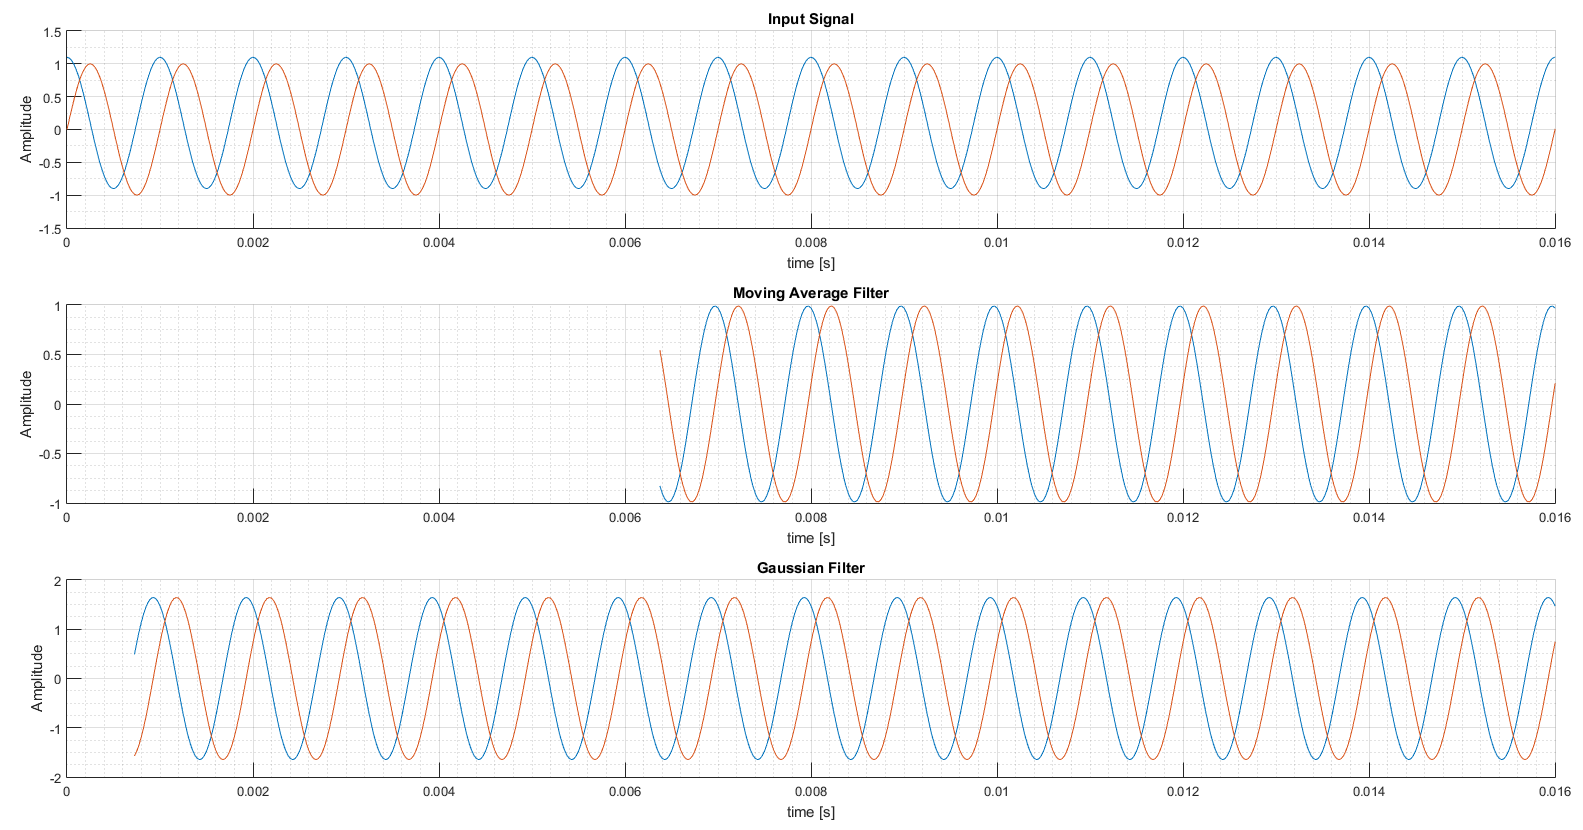
\includegraphics[width=\textwidth]{plots/dc_comp.png}
   		 		\caption{\textit{Comparison of DC offset algorithms outputs in time domain.}}
			\end{figure}
			\vspace{1cm}		
			\begin{figure}[!htb]
    			\centering
   				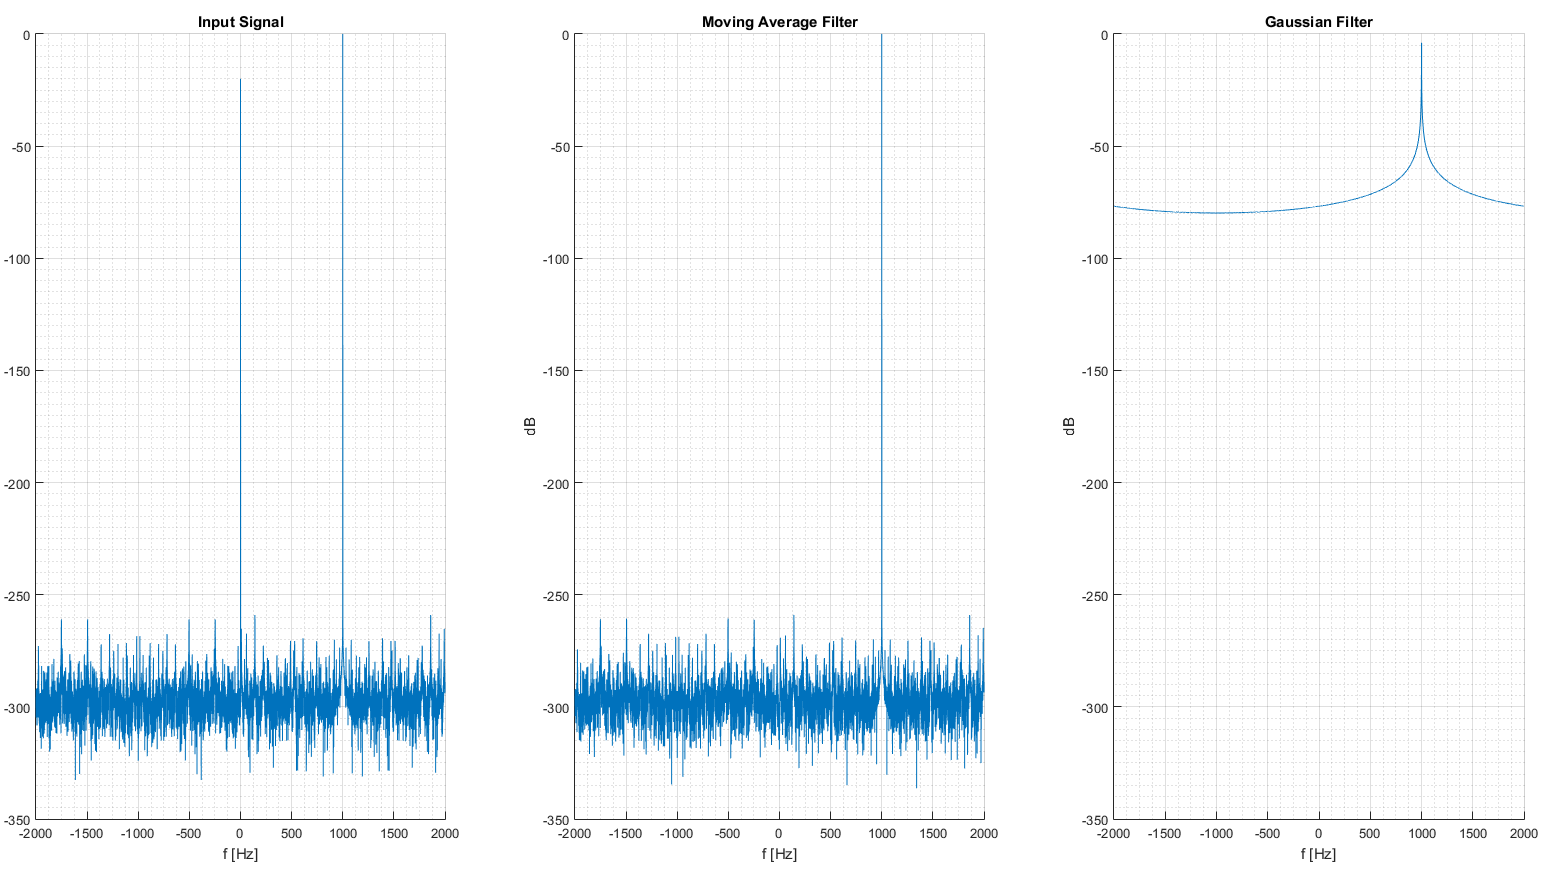
\includegraphics[width=\textwidth]{plots/dc_f.png}
   		 		\caption{\textit{Comparison of DC offset algorithms outputs in frequency domain.}}
			\end{figure}		
			\begin{figure}[!htb]
    			\centering
   				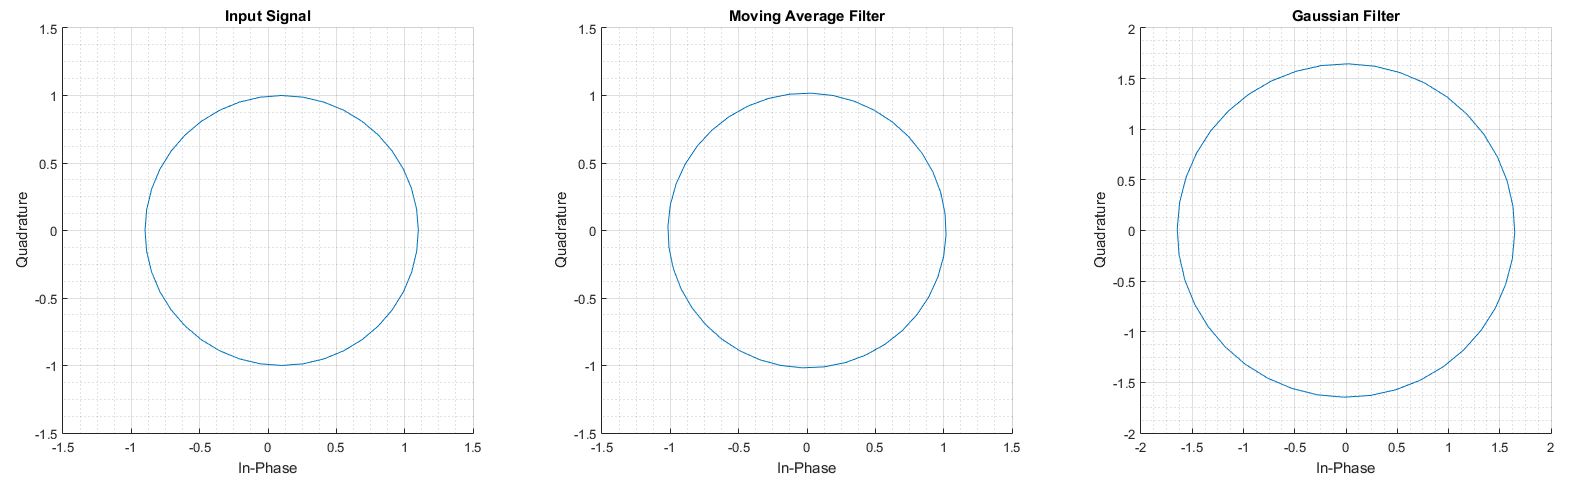
\includegraphics[width=\textwidth]{plots/dc_c.png}
   		 		\caption{\textit{Comparison of constellation diagram for tested algorithms.}}
			\end{figure}
			
		\subsubsection*{Scenario 1: Noisy signal}
		\begin{figure}[H]
    			\centering
   				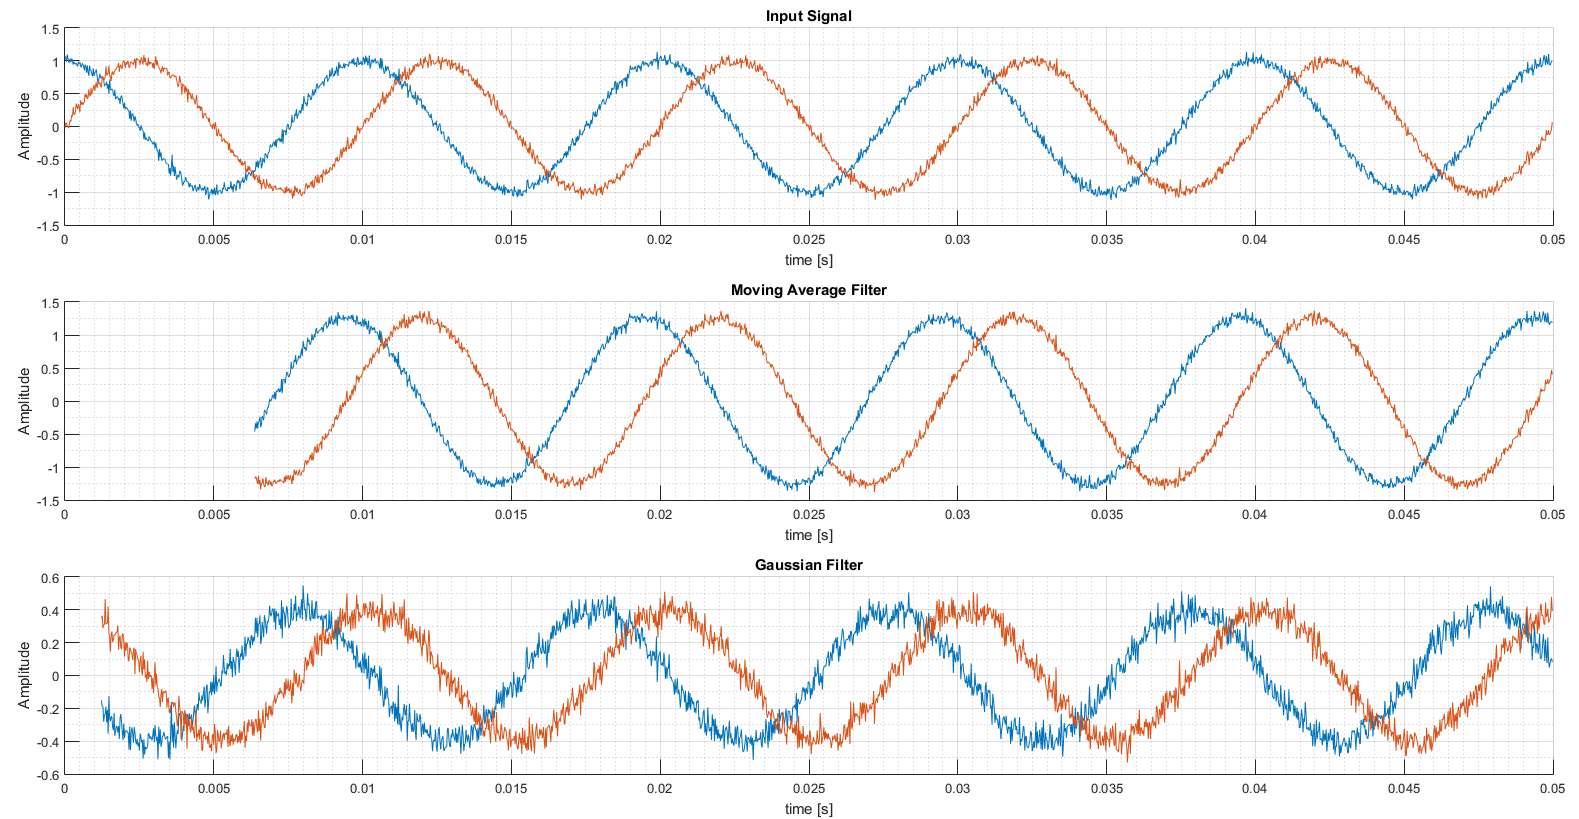
\includegraphics[width=\textwidth]{plots/dc_comp_n.png}
   		 		\caption{\textit{Comparison of DC offset algorithms outputs in time domain.}}
		\end{figure}		
		\begin{figure}[H]
    			\centering
   				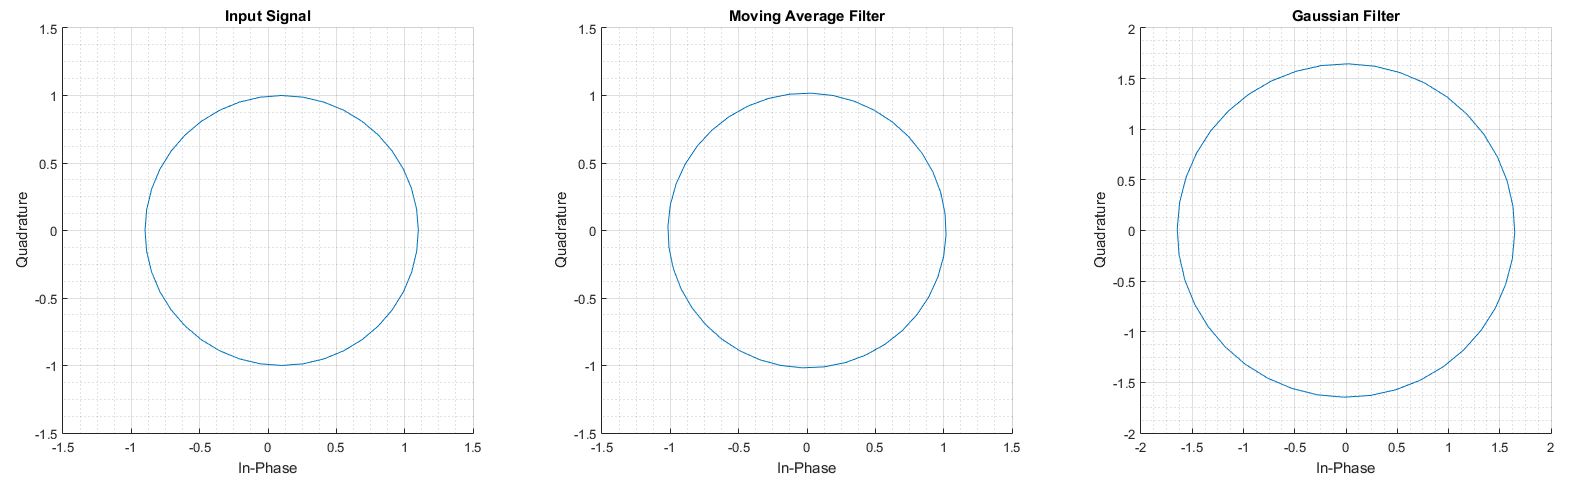
\includegraphics[width=\textwidth]{plots/dc_c.png}
   		 \caption{\textit{Comparison of constellation diagram for tested algorithms.}}
		\end{figure}
		\begin{figure}[H]
    			\centering
   				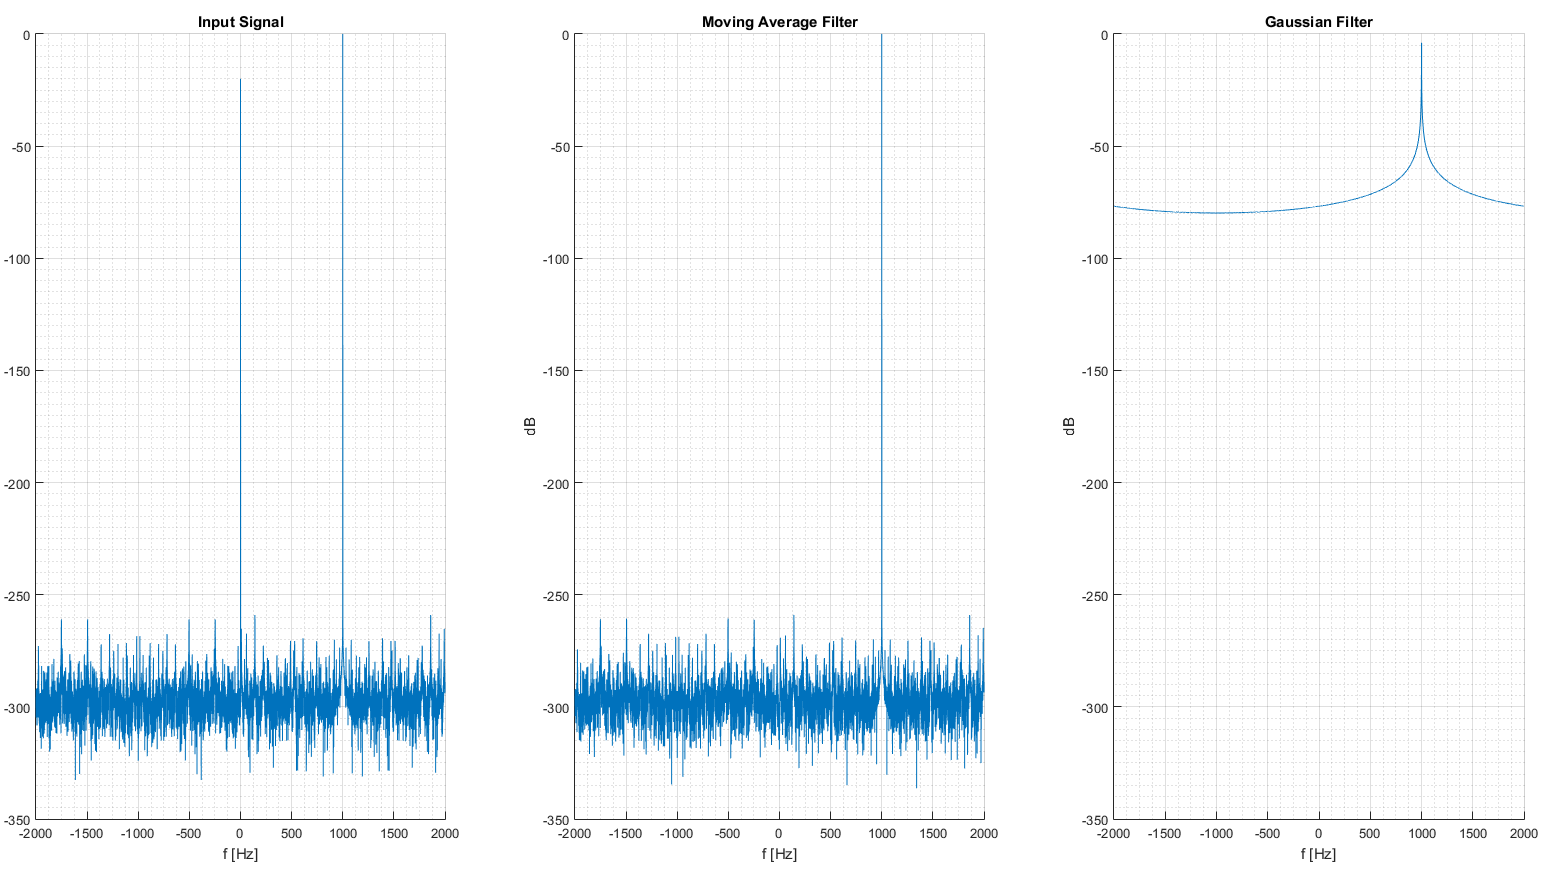
\includegraphics[width=\textwidth]{plots/dc_f.png}
   		 		\caption{\textit{Comparison of DC offset algorithms outputs in frequency domain.}}
		\end{figure}
		Gaussian filters needs almost three times lower number of samples to work correctly in
		comparison to Moving Average Filter. It means lower delay in processing path. Gaussian
		filter distort magnitude of the signal, but this problem will be resolved by Magnitude and
		Phase correction algorithm.
	\newpage
	\subsection*{Single Tone Signal}
		In this case IQ mismatch compensation with two DC offset removal algorithms are compared for
		single tone signal with frequency $f=1kHz$ with and without additional noise.
		\subsubsection*{Scenario 1: Noiseless signal}
			\begin{figure}[!htb]
    			\centering
   				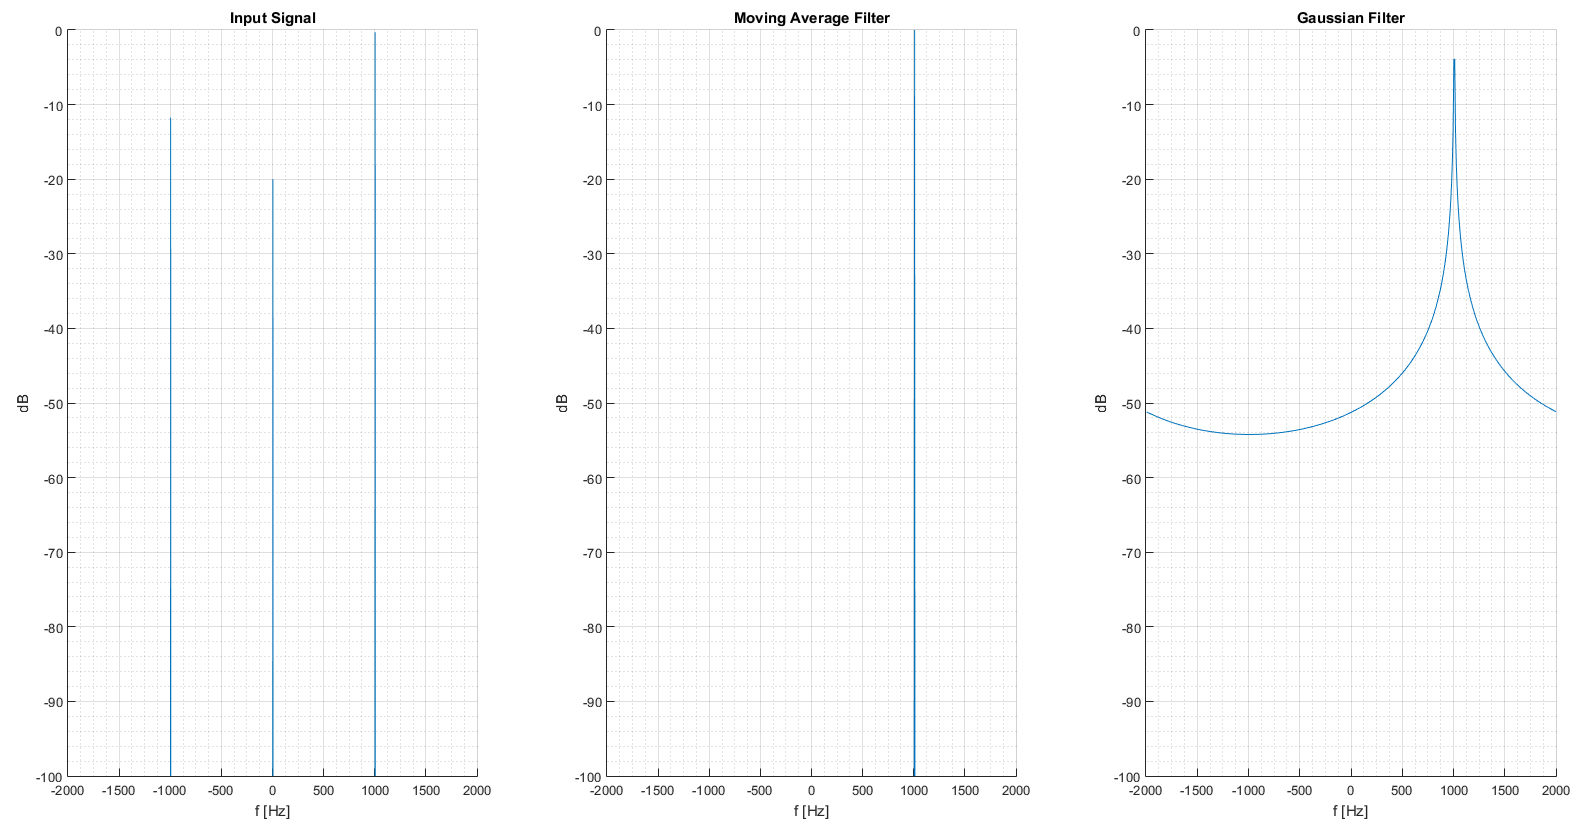
\includegraphics[width=\textwidth]{plots/single_f.png}
   		 		\caption{\textit{Comparison of spectrum for IQ mismatch compensation algorithms 
   		 		for signle tone signal.}}
   		 	\end{figure}
   		 	\vspace{1cm}
   		 	\begin{figure}[H]
    			\centering
   				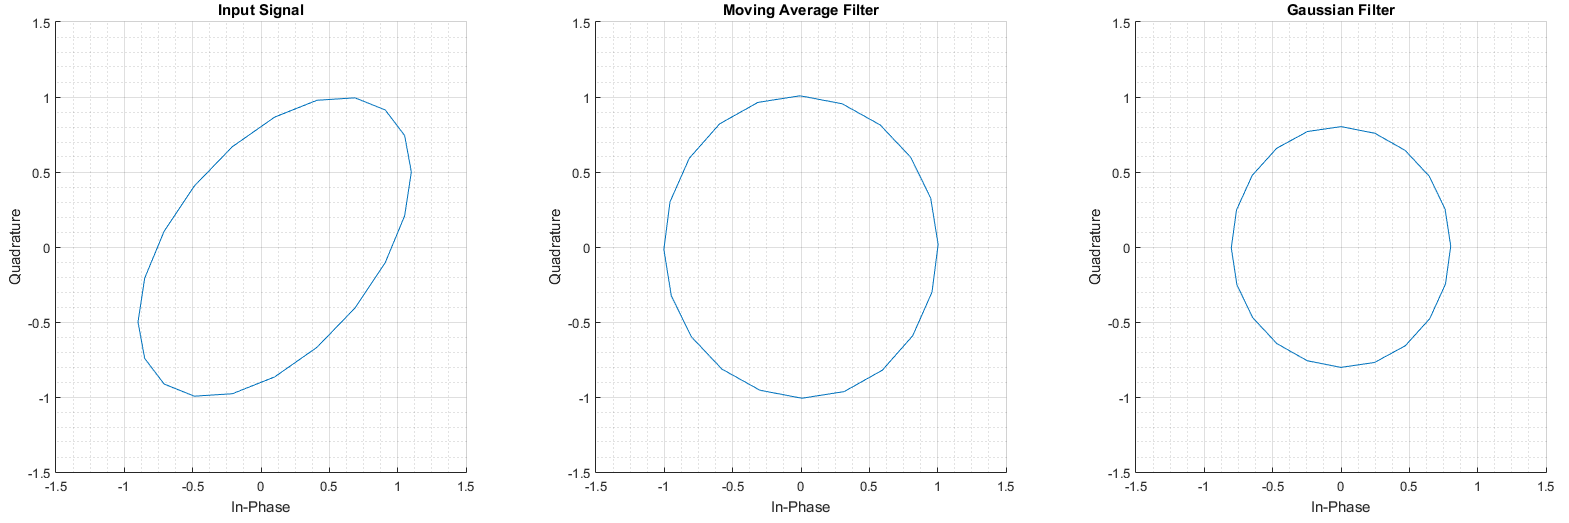
\includegraphics[width=\textwidth]{plots/single_c.png}
   		 		\caption{\textit{Comparison of constellations for IQ mismatch compensation algorithms 
   		 		for signle tone signal.}}
			\end{figure}
		\newpage
		\newpage
		\subsubsection*{Scenario 2: Noisy signal}
			\vspace{1cm}
			\begin{figure}[H]
    			\centering
   				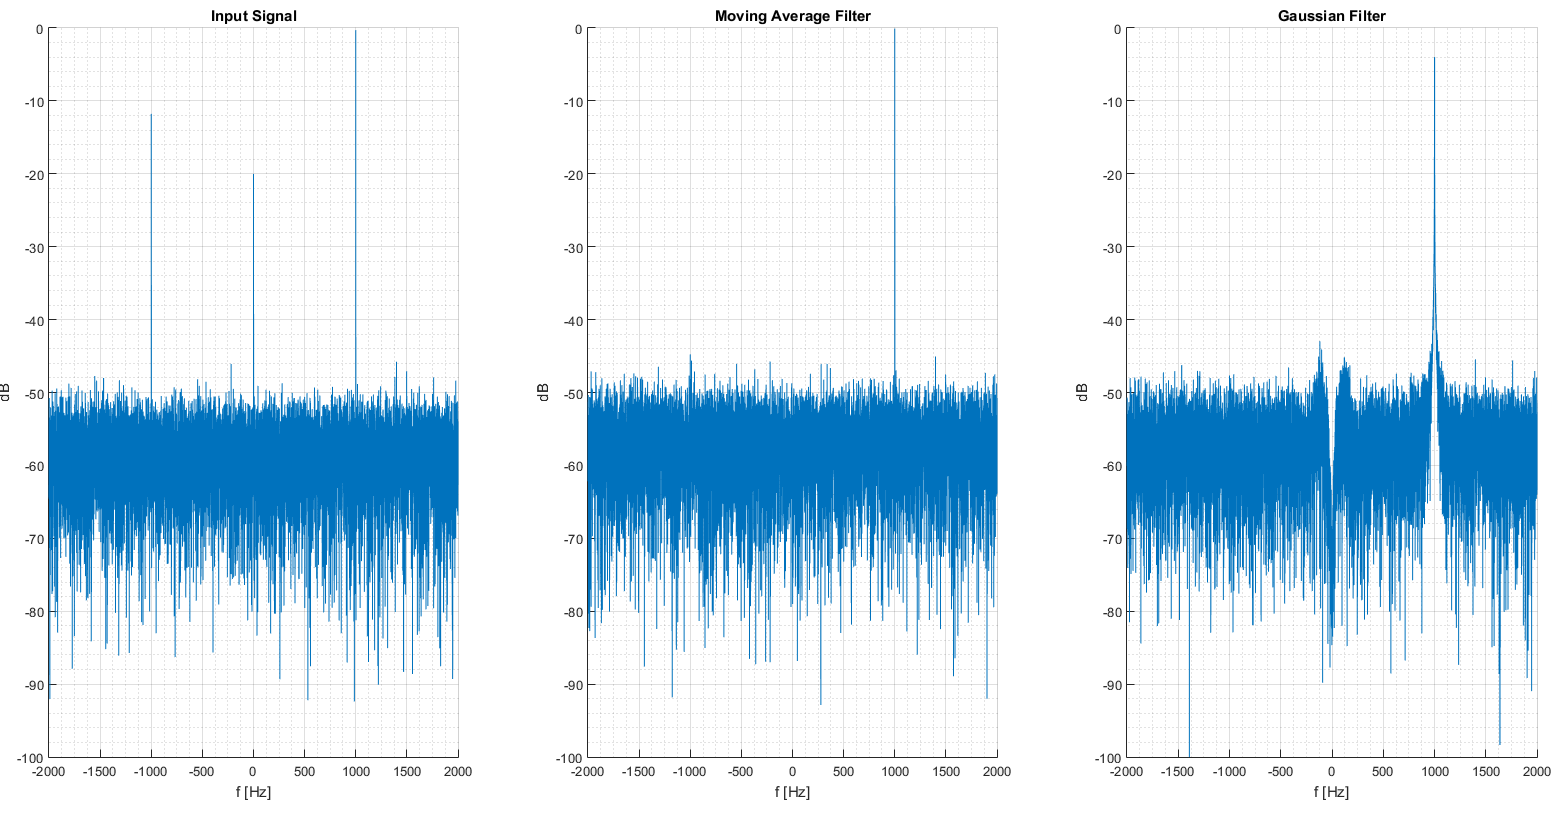
\includegraphics[width=\textwidth]{plots/single_nf.png}
   		 		\caption{\textit{Comparison of spectrum for IQ mismatch compensation algorithms 
   		 		for signle tone signal with noise.}}
   		 	\end{figure}	
   		 	\vspace{2cm}
   		 	\begin{figure}[H]
    			\centering
   				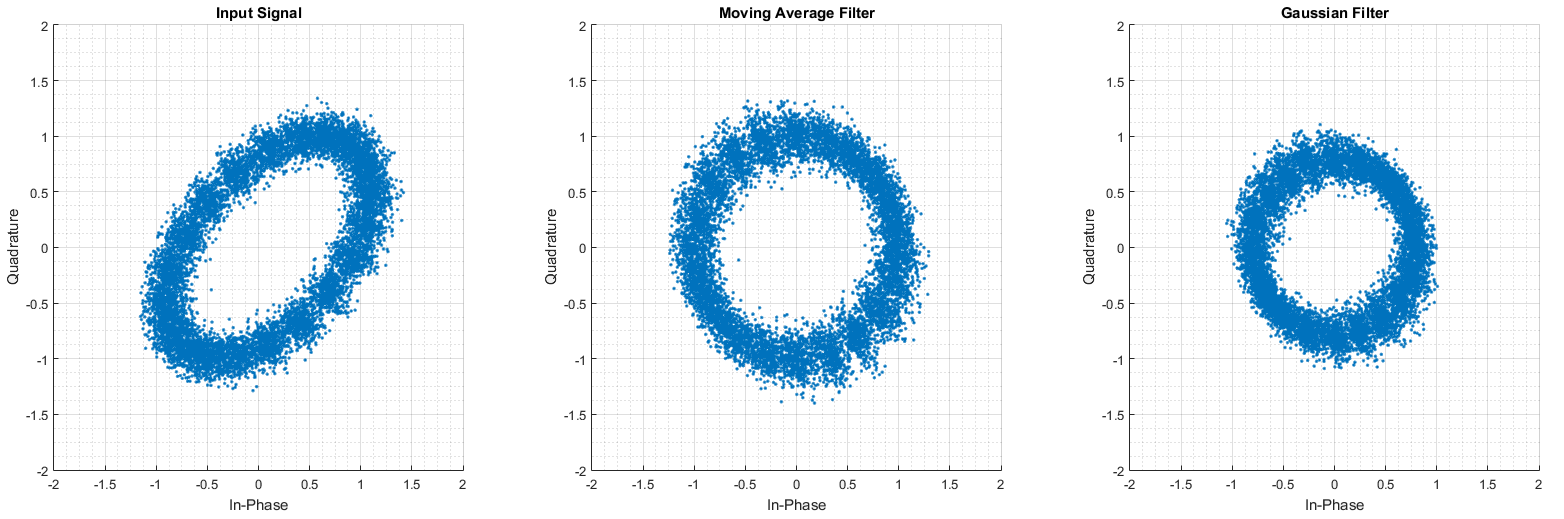
\includegraphics[width=\textwidth]{plots/single_nc.png}
   		 		\caption{\textit{Comparison of constellations for IQ mismatch compensation algorithms 
   		 		for signle tone signal with noise.}}
   		 	\end{figure}
   		 	
   		 	In both cases unwanted image in $-1kHz$ and DC component were removed.
   		 	Gaussian Filter introduced some spectral leakage, but compensation was still
   		 	working correctly. Constellation diagram after mismatch correction is visibly
   		 	shaper closer to circle than before. 
   	\newpage
   	\subsection*{Multi tone}
   		In this case IQ mismatch compensation with two DC offset removal algorithms are compared for
		multi tone signal with frequencies $f1=1kHz$ and $f2=0.5kHz$ with and without additional noise.
		\subsubsection*{Scenario 1: Noiseless signal}\
			\begin{figure}[!htb]
    			\centering
   				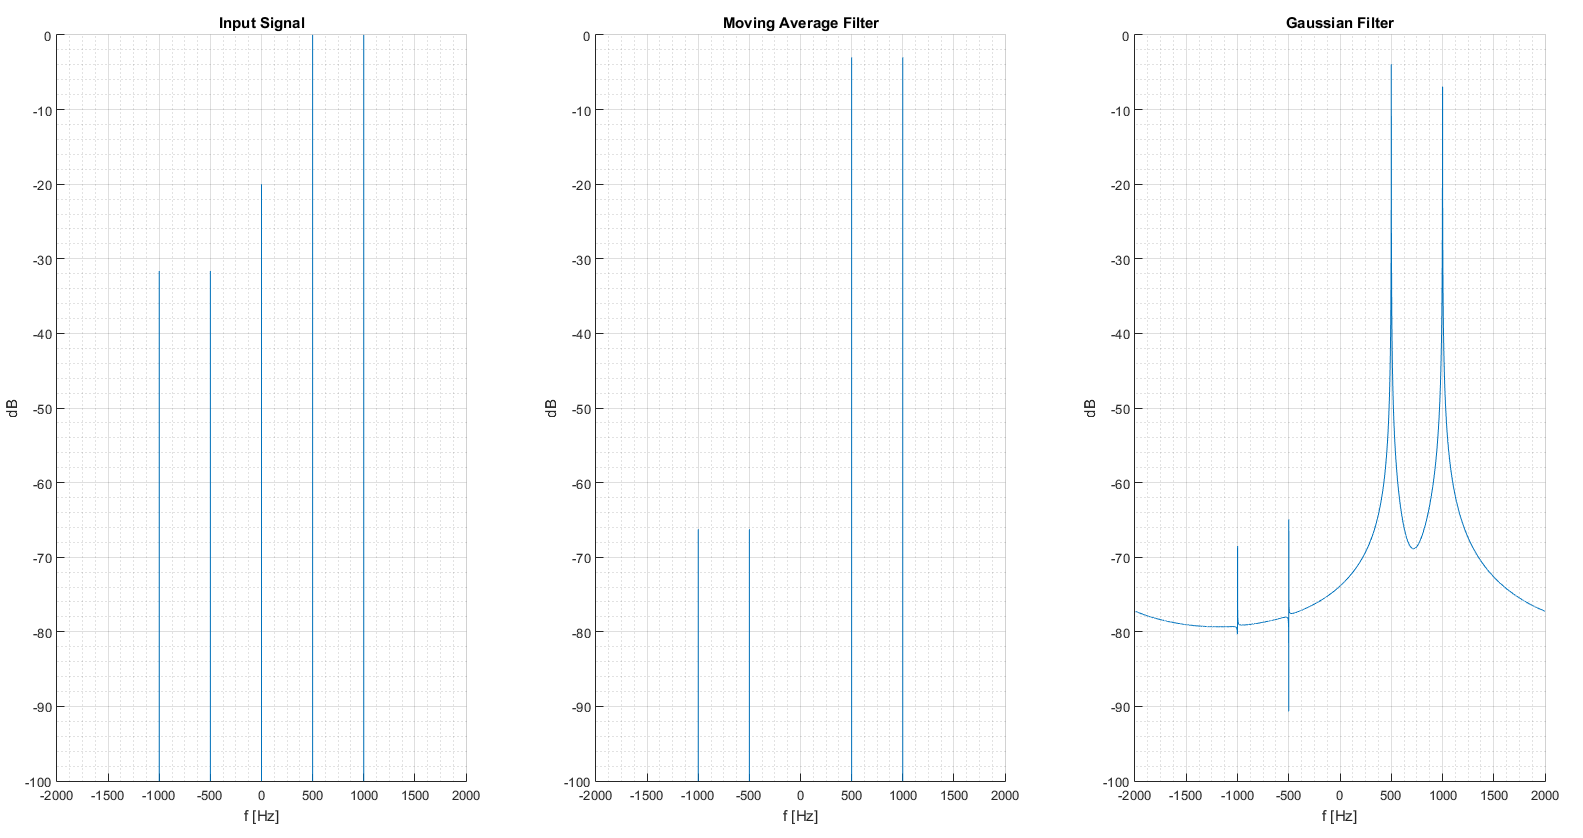
\includegraphics[width=\textwidth]{plots/multi_f.png}
   		 		\caption{\textit{Comparison of spectrum for IQ mismatch compensation algorithms 
   		 		for multi tone signal.}}
   		 	\end{figure}	
   		 	\begin{figure}[!htb]
    			\centering
   				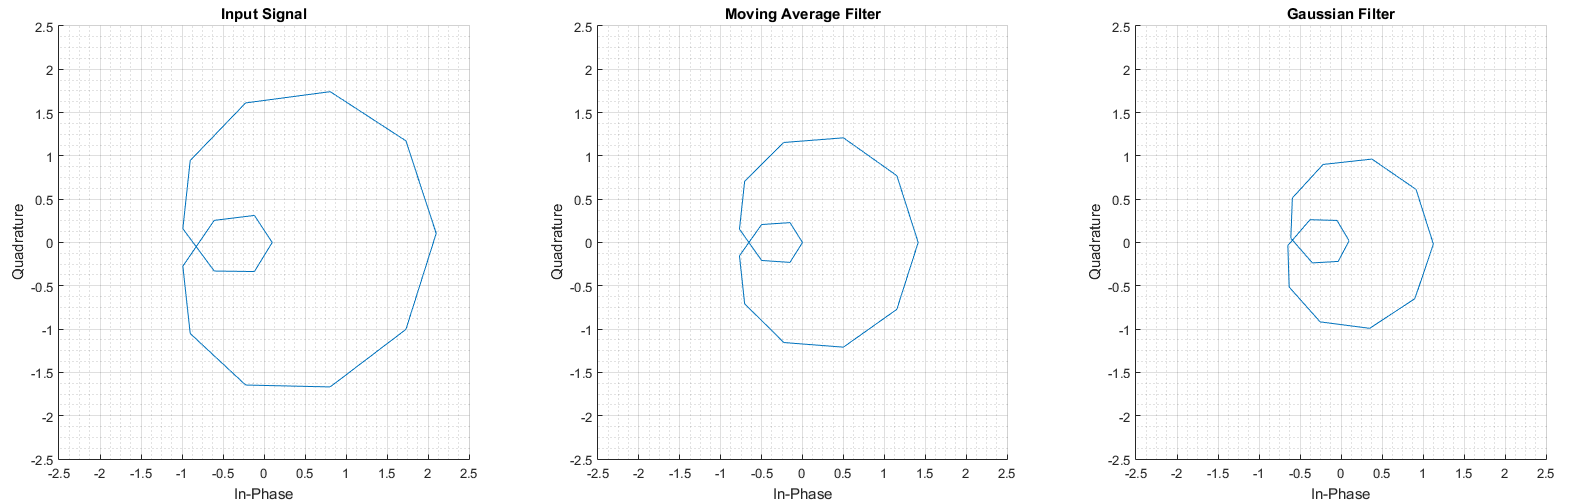
\includegraphics[width=\textwidth]{plots/multi_c.png}
   		 		\caption{\textit{Comparison of constellations for IQ mismatch compensation algorithms
   		 		for multi tone.}}
   		 	\end{figure}		
		\subsubsection*{Scenario 1: Noisy signal}
			\vspace{1cm}
			\begin{figure}[H]
    			\centering
   				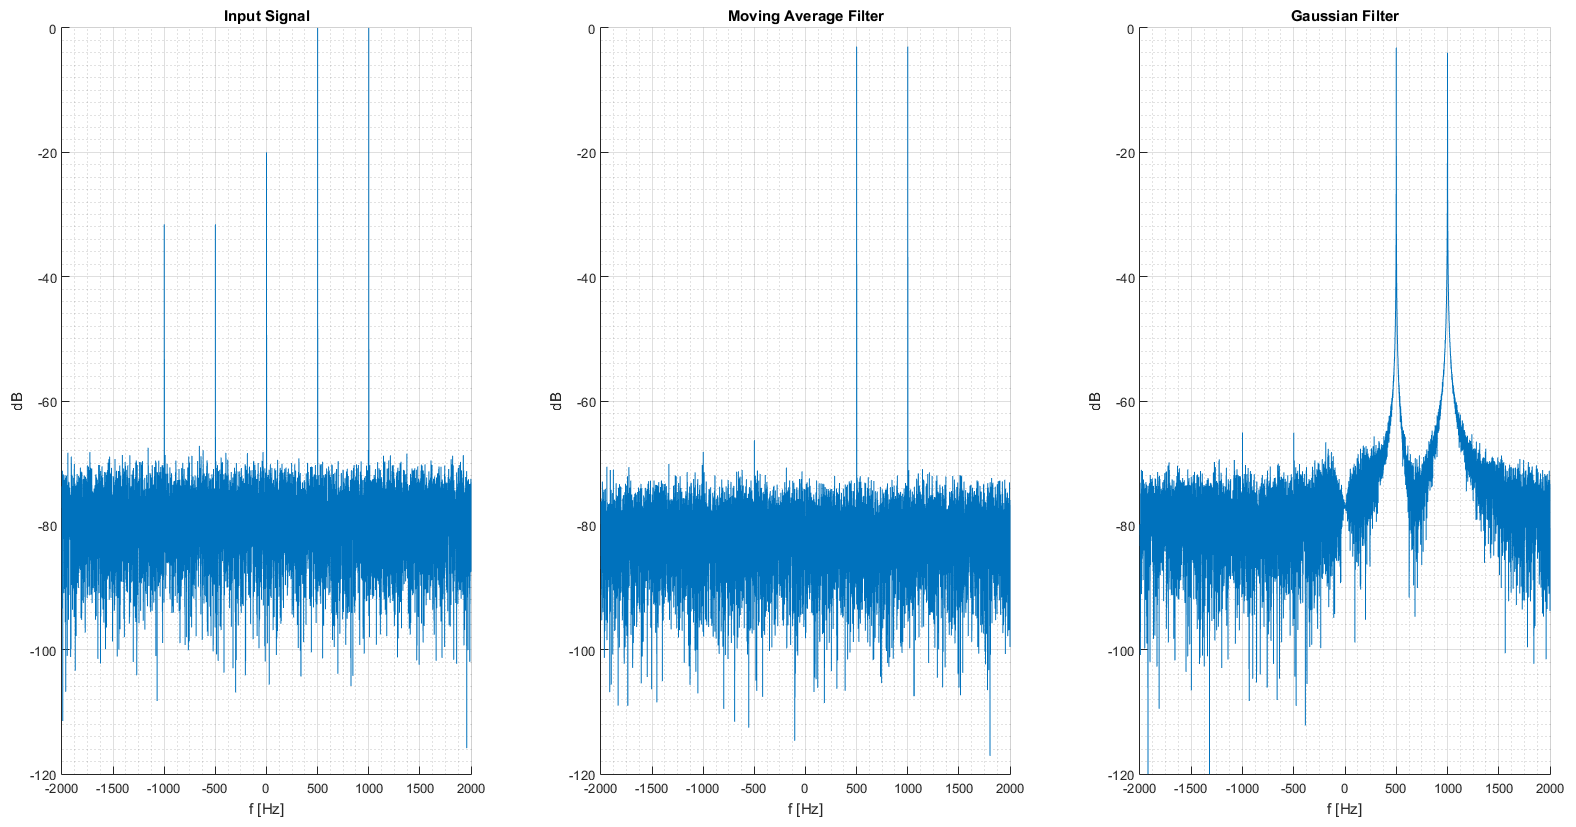
\includegraphics[width=\textwidth]{plots/multi_nf.png}
   		 		\caption{\textit{Comparison of spectrum for IQ mismatch compensation algorithms for 
   		 		multi tone signal with noise.}}
   		 	\end{figure}
   		 	\vspace{2cm}	
   		 	\begin{figure}[H]
    			\centering
   				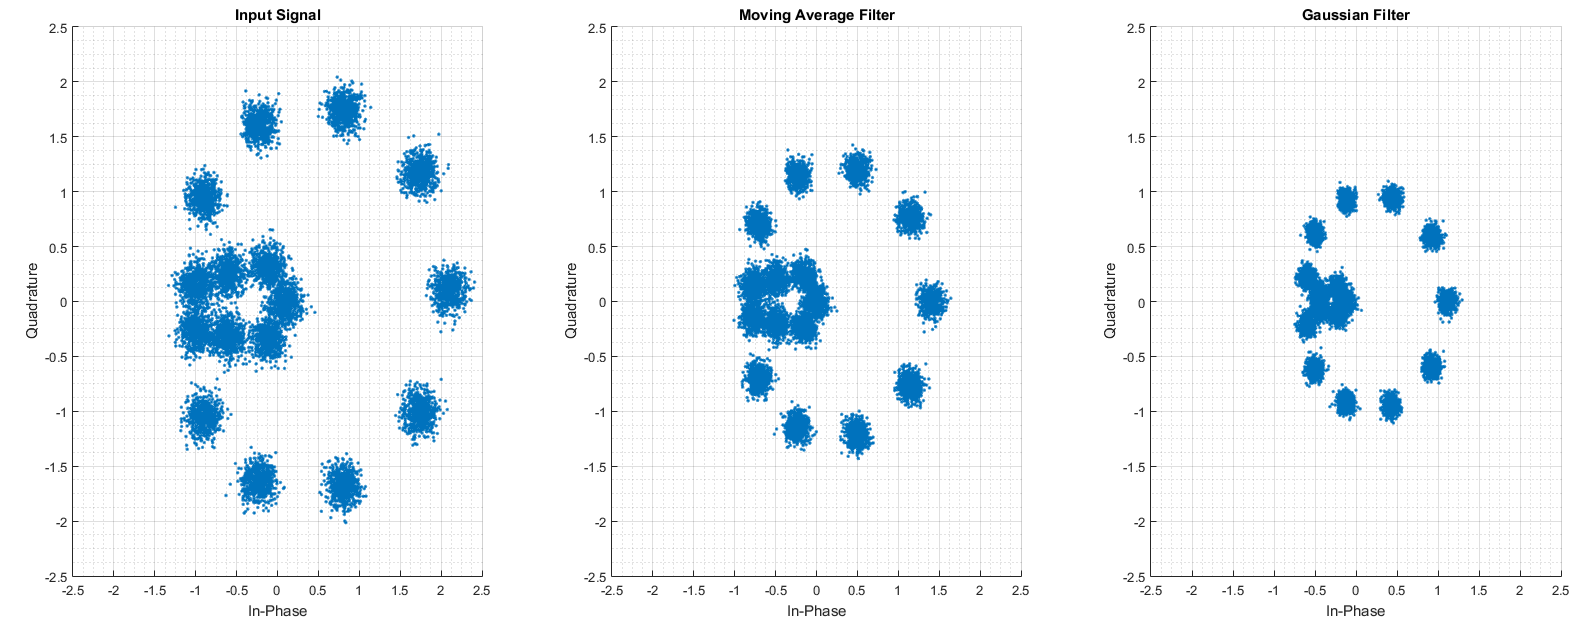
\includegraphics[width=\textwidth]{plots/multi_nc.png}
   		 		\caption{\textit{Comparison of constellations for IQ mismatch compensation algorithms 
   		 		for multi tone signal with noise.}}
   		 	\end{figure}
   		 	
   		 	Signal image and DC offset were successfully removed by correction algorithms. Again,
   		 	Gaussian filter introduced some spectral leakage. In this case constellation diagram
   		 	is composed of two circles each representing different frequency in the signal.
   		 	
   	\newpage
	\subsection*{Broadband}
		In this case IQ mismatch compensation with two DC offset removal algorithms are compared for
		broadband signal in frequency range from $f_s=0.5kHz$ to $f_e=1kHz$ with and without additional
		noise.
		\subsubsection*{Scenario 1: Noiseless signal}
			\begin{figure}[!htb]
    			\centering
   				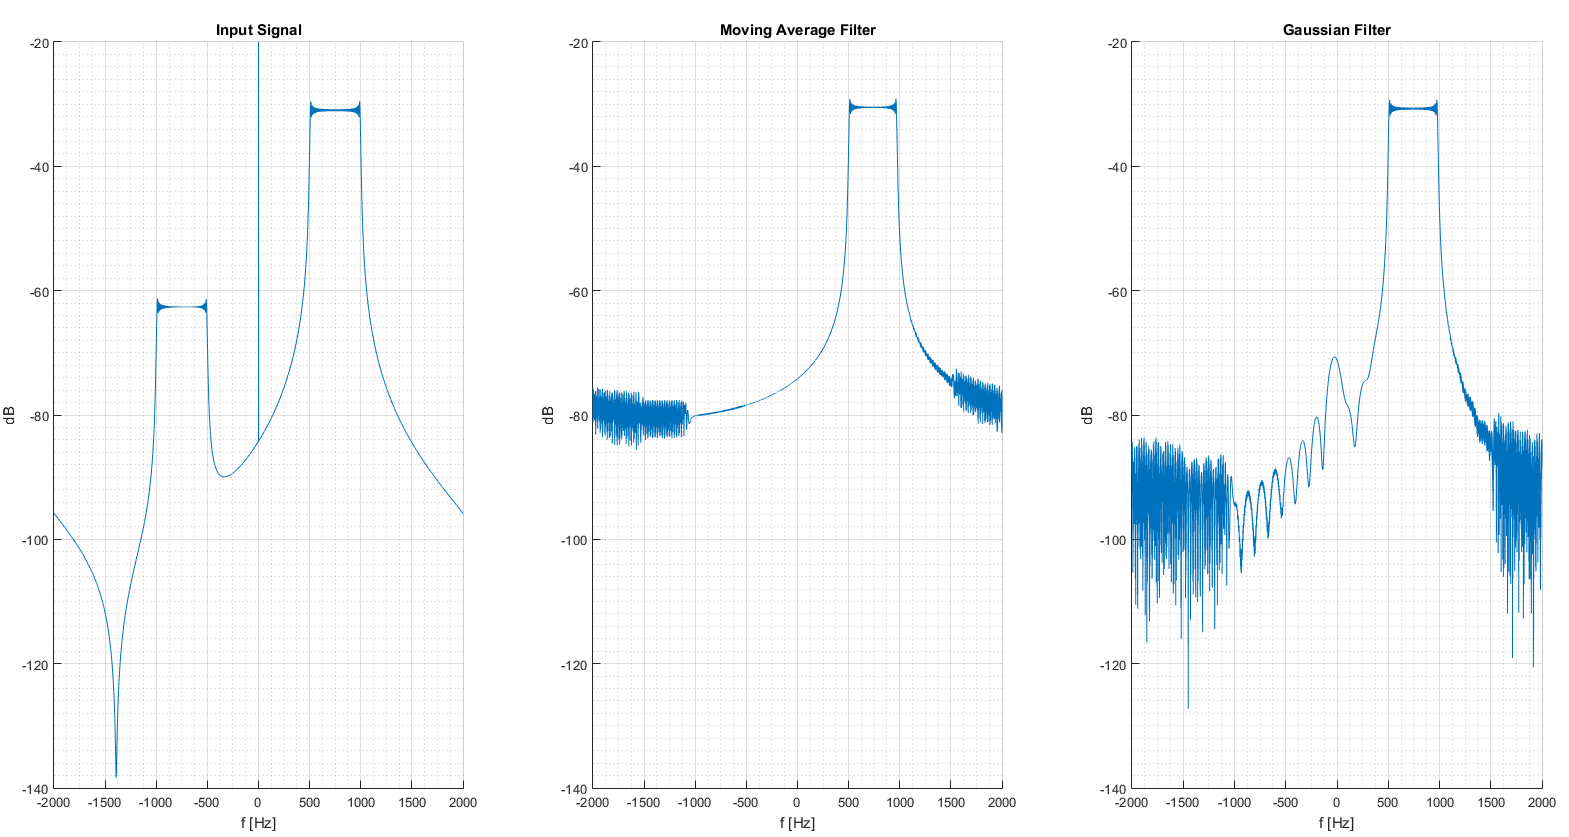
\includegraphics[width=\textwidth]{plots/band_f.png}
   		 		\caption{\textit{Comparison of spectrum for IQ mismatch compensation algorithms for
   		 		broadband signal.}}
   		 	\end{figure}	
   		 	\begin{figure}[!htb]
    			\centering
   				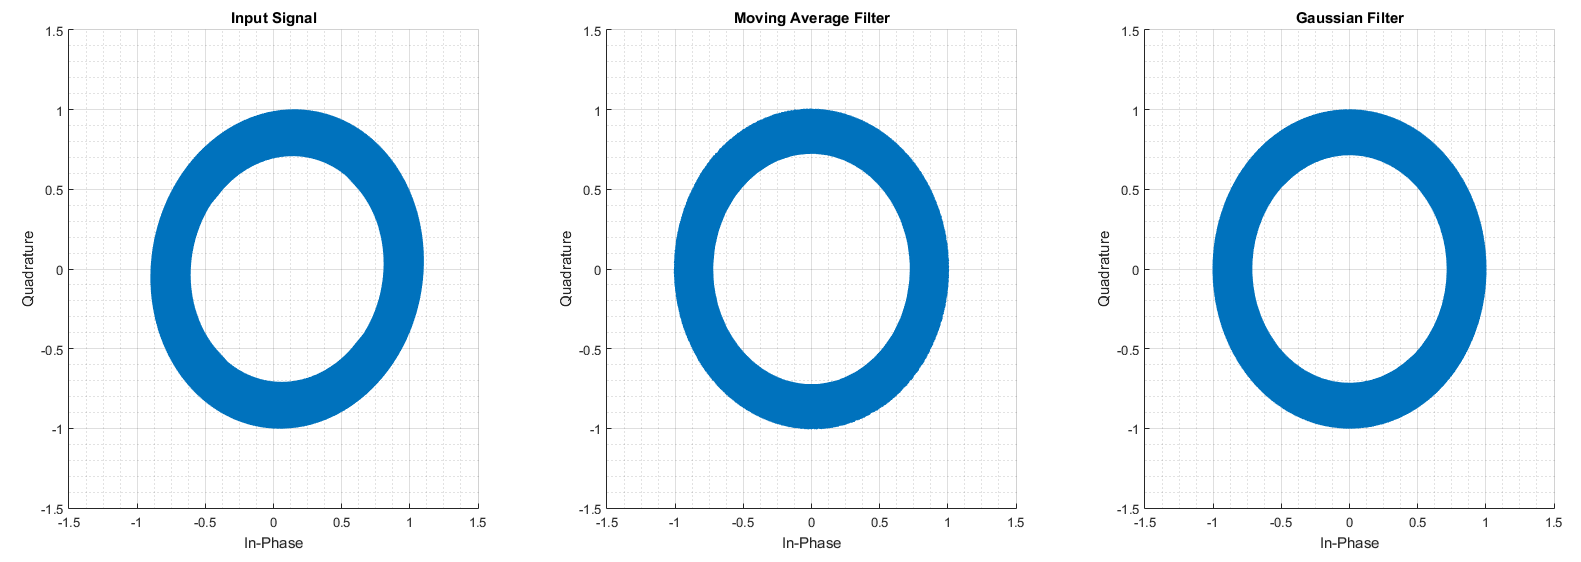
\includegraphics[width=\textwidth]{plots/band_c.png}
   		 		\caption{\textit{Comparison of constellations for IQ mismatch compensation algorithms 
   		 		for broadband signal.}}
   		 	\end{figure}
   		\newpage
		\subsubsection*{Scenario 1: Noisy signal}
			\begin{figure}[!htb]
    			\centering
   				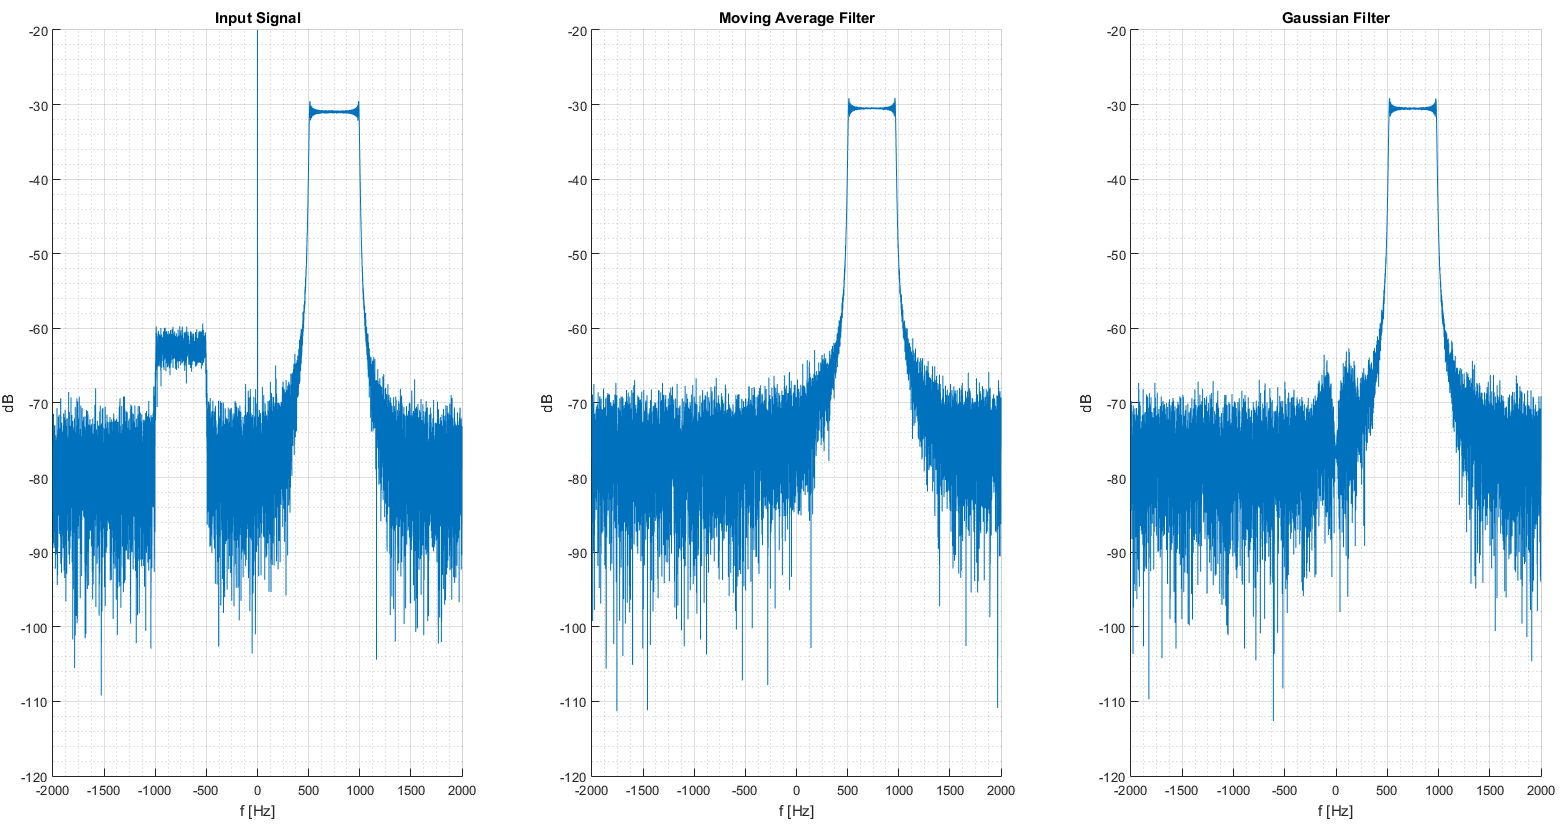
\includegraphics[width=\textwidth]{plots/band_nf.png}
   		 		\caption{\textit{Comparison of spectrum for IQ mismatch compensation algorithms for
   		 		broadband signal with noise.}}
   		 	\end{figure}	
   		 	\begin{figure}[!htb]
    			\centering
   				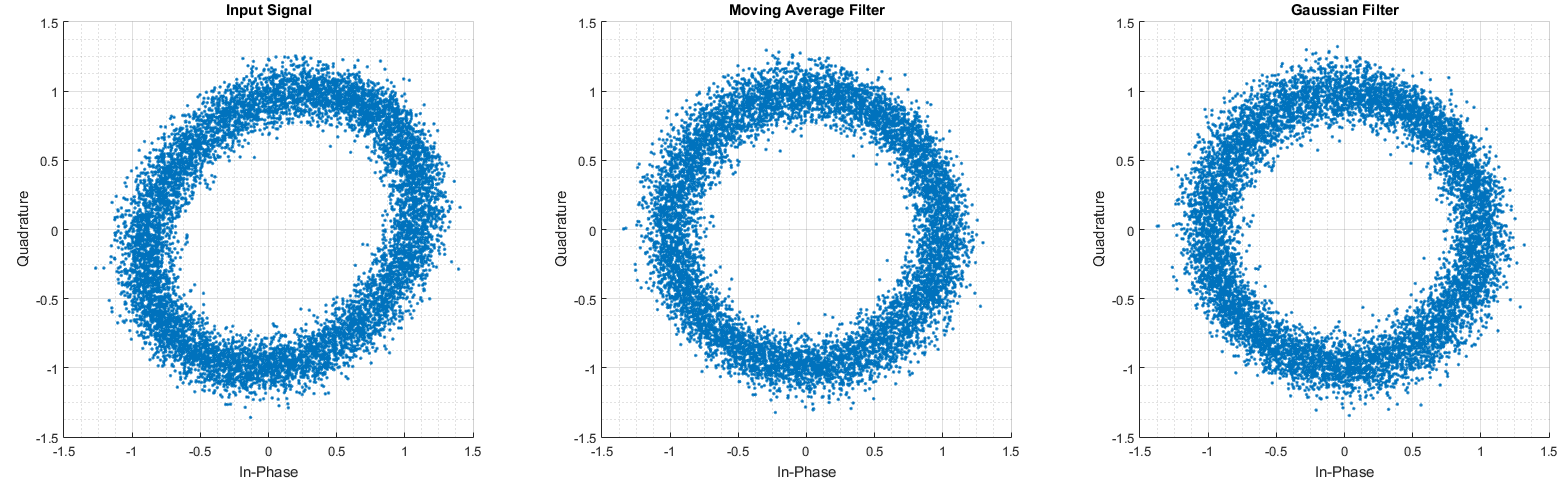
\includegraphics[width=\textwidth]{plots/band_nc.png}
   		 		\caption{\textit{Comparison of constellations for IQ mismatch compensation algorithms 
   		 		for broadband signal with noise.}}
   		 	\end{figure}
   		 	
			Signal image and band from $-1kHz$ to $-0.5kHz$ and DC offset were successfully removed.
			Constellation diagram shows improvement in signal orthogonality. In this case constellation
			diagram is a ring which starts at lower band limit and ends at upper band limit.    		 	
   		 	
   	\newpage	
	\section{Hardware Implementation}
		This section contains description of all algorithms implemented in Zynq PL section and its 
		performance evaluation.
		All test were performed using IIO Oscilloscope program.
		Transmit and receive path are configured as follows:
		\begin{itemize}
			\item sampling rate - $30.719998$ MSPS,
			\item bandwidth - $18MHz$.,
			\item TX LO frequency - $2799.999998$ MHz,
			\item RX LO frequency - $2799.999998$ MHz.
		\end{itemize}
		and in following conditions:
		\begin{itemize}
			\item Moving Average Filter Order - 256.
			\item Gaussian filter $\sigma$ = 5, window size = 30
			\item Amplitude - 1,
			\item DC offset in I branch - 0.1,
			\item Phase mismatch - 3$^\circ$.
		\end{itemize}
	\newpage
	 \subsection*{DC offset removal}
	 	In this case built in DC offset correction algorithm is tested for signle tone
		signal of frequency $f=1kHz$.
	 	\begin{figure}[H]
    		\centering
   			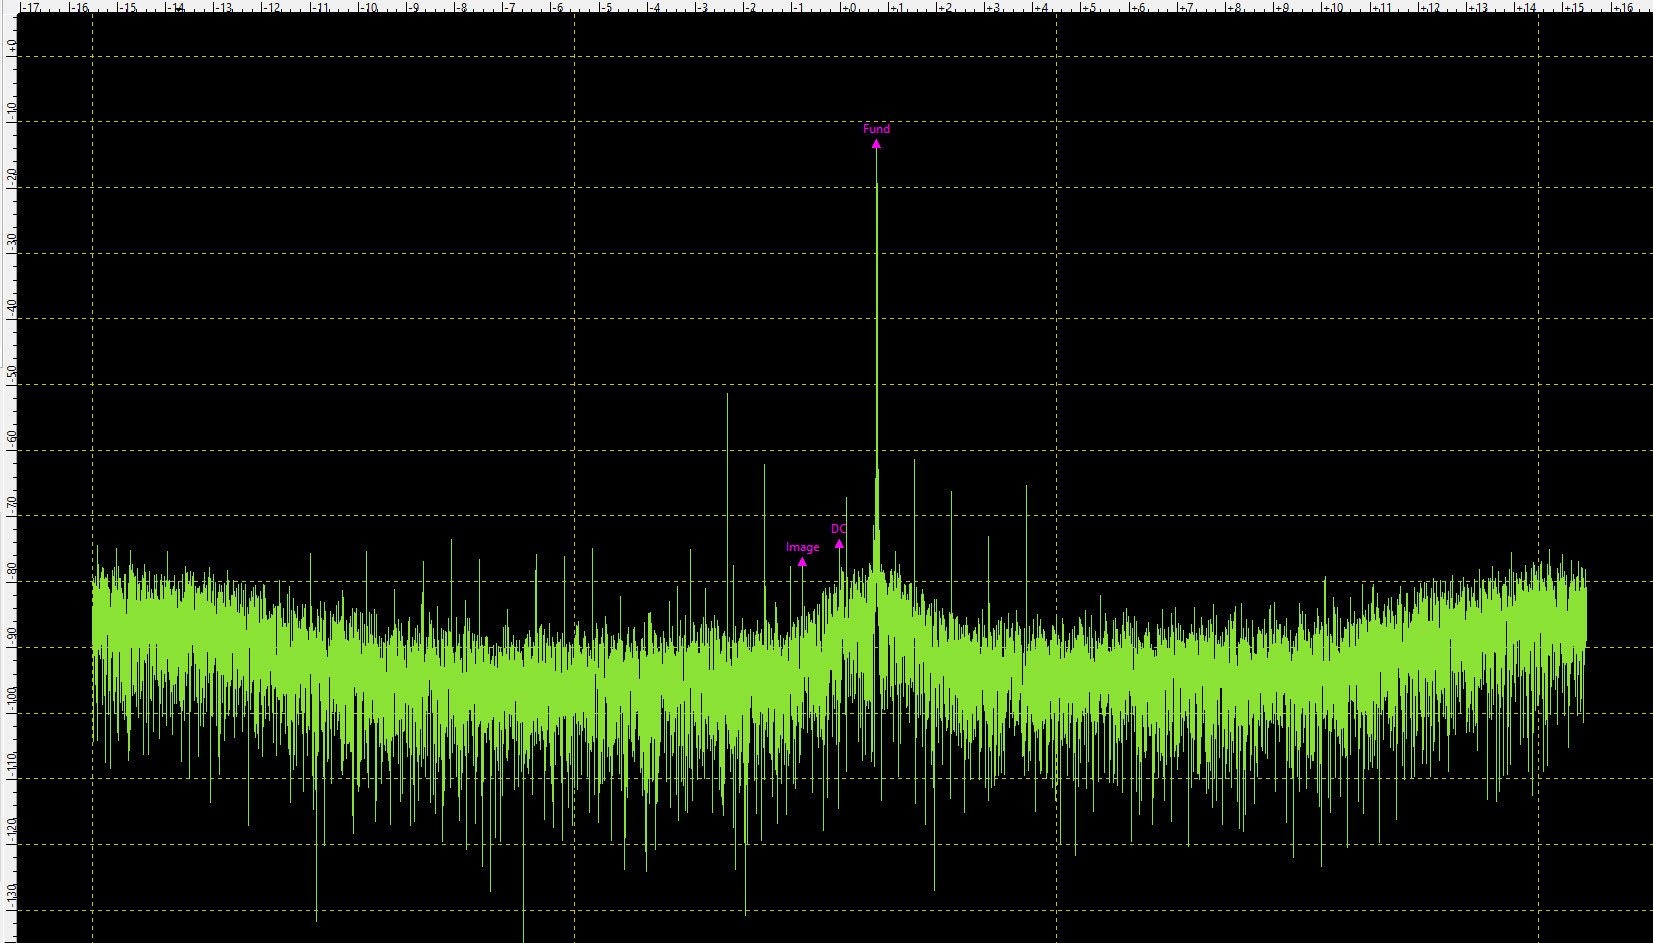
\includegraphics[width=\textwidth]{plots/my_dc.png}
   		 	\caption{\textit{Received signal spectrum with Moving Average Filter DC offset removal
   		 	implemented in Zynq PL section.}}
   		\end{figure}
   		
	 	\begin{figure}[H]
    		\centering
   			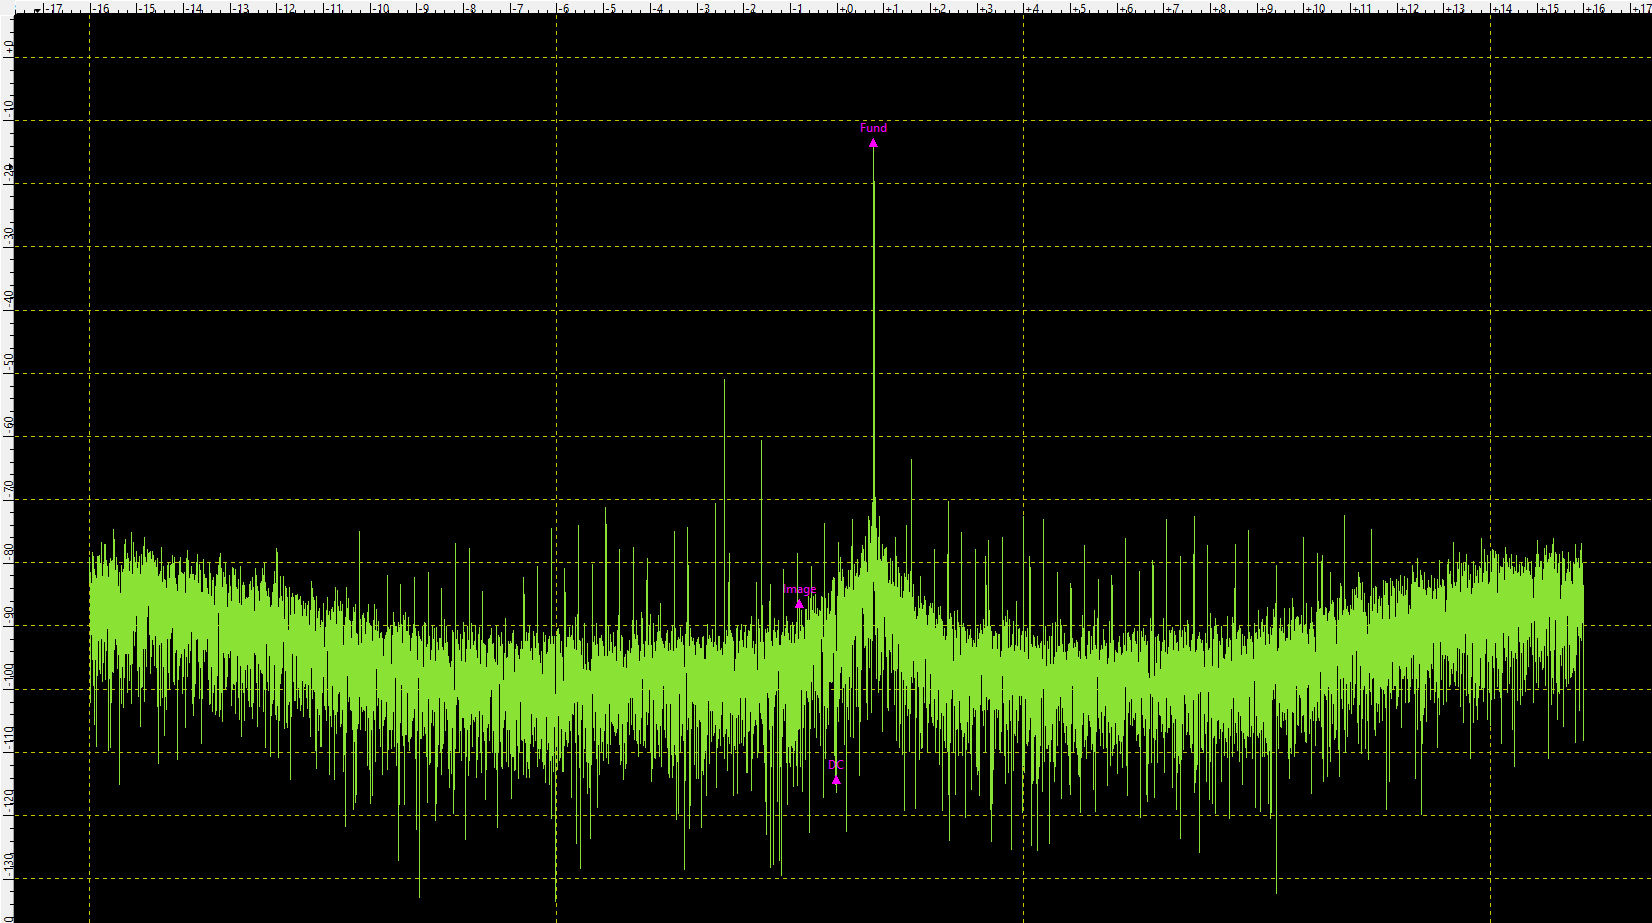
\includegraphics[width=\textwidth]{plots/my_dc_gauss.png}
   		 	\caption{\textit{Received signal spectrum with Gaussian Filter DC offset removal
   		 	implemented in Zynq PL section.}}
   		\end{figure}
   		
		\subsection*{Single Tone Signal}
		In this case implemented mismatch compensation is tested for
		single tone signal with frequency $f=1kHz$.
		\begin{figure}[!htb]
    		\centering
   			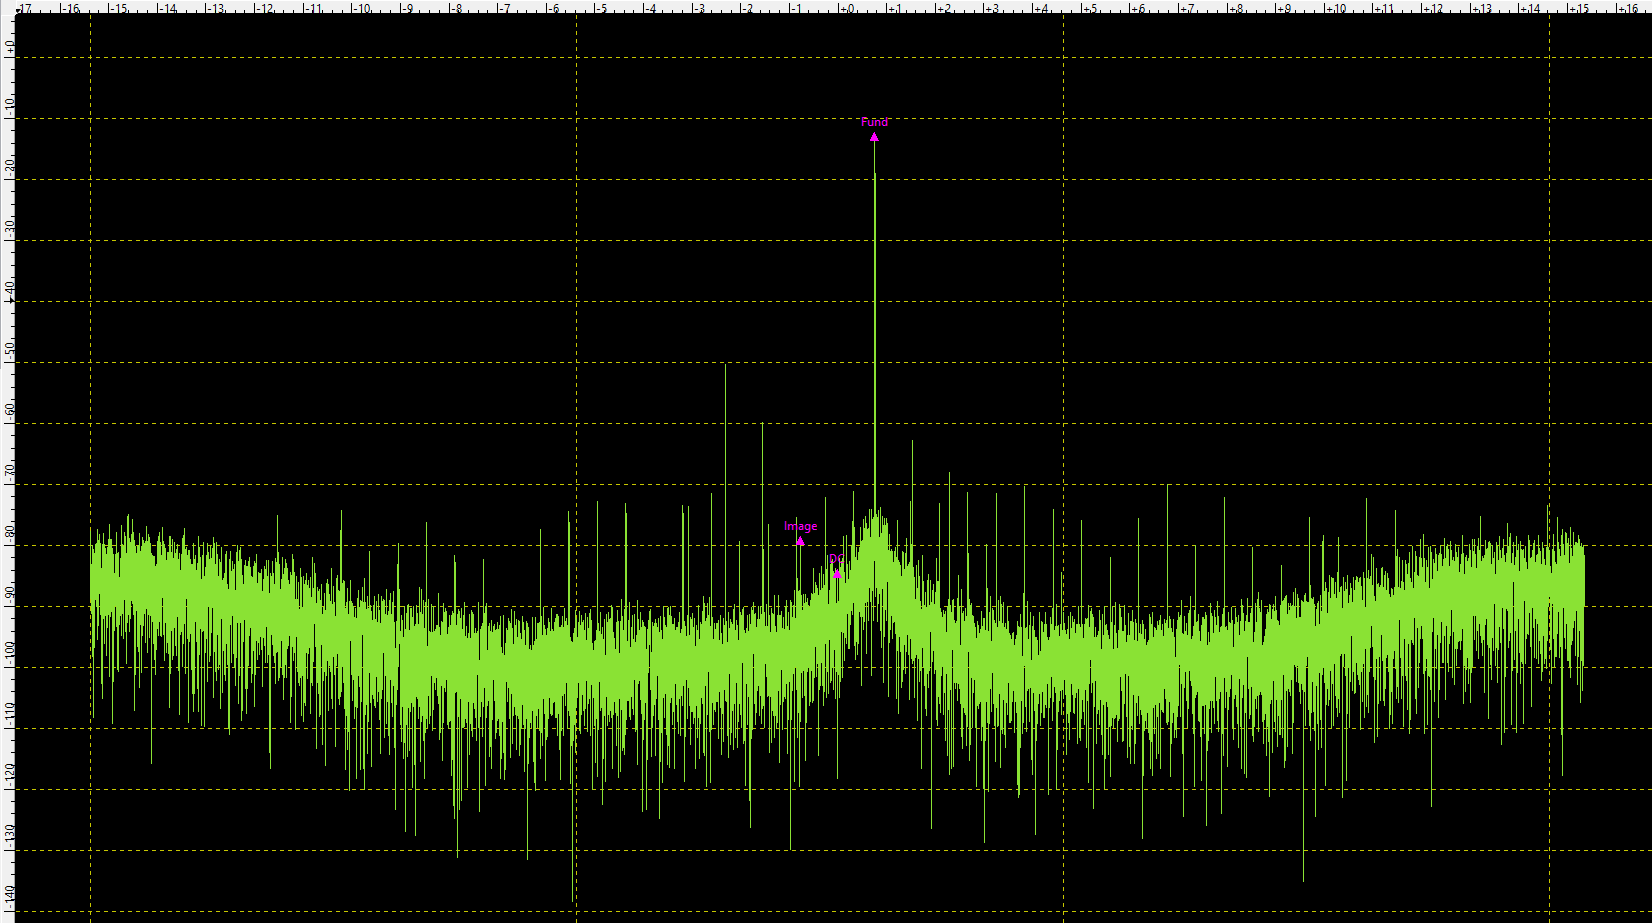
\includegraphics[width=\textwidth]{plots/my_single_mav.png}
   		 	\caption{\textit{Received single tone signal spectrum with IQ mismatch compensation with
   		 	Moving Average Filter.}}
   		\end{figure}
   		
   		\begin{figure}[!htb]
    		\centering
   			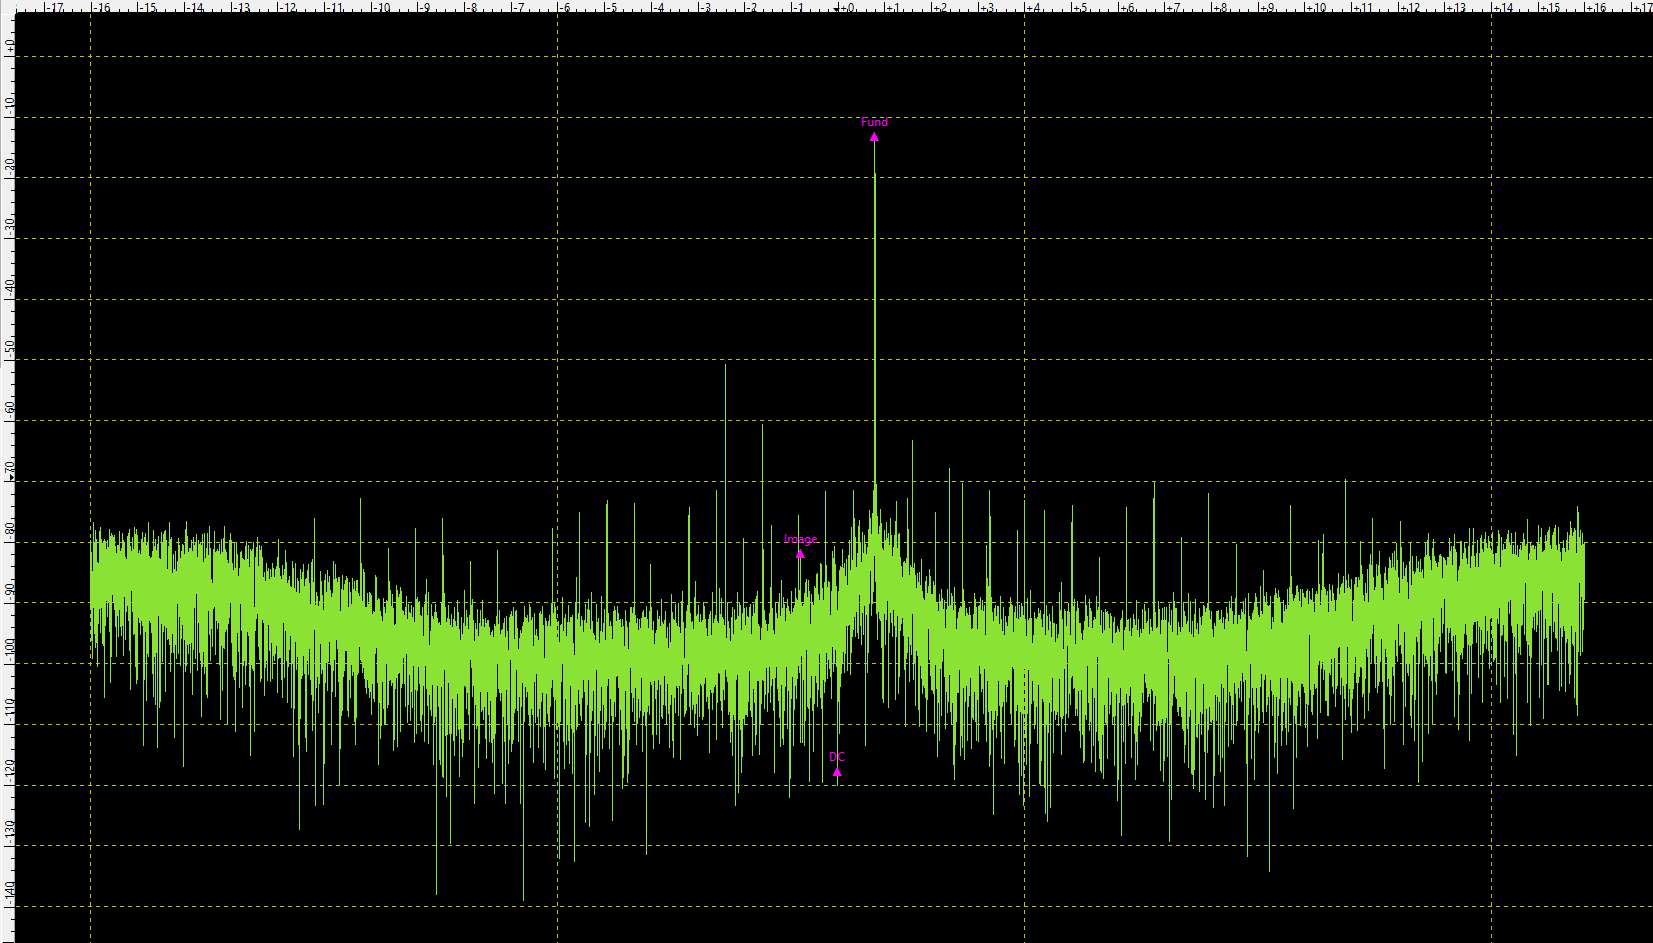
\includegraphics[width=\textwidth]{plots/my_single_gauss.png}
   		 	\caption{\textit{Received broadband signal spectrum with IQ mismatch compensation with
   		 	Gaussian Filter.}}
   		\end{figure}	
   		
   		\subsection*{Multiton Signal}
   		In this case implemented mismatch compensation is tested for
		multi tone signal with frequencies $f1=1kHz$ and $f2=0.5kHz$.
  		\begin{figure}[!htb]
    		\centering
   			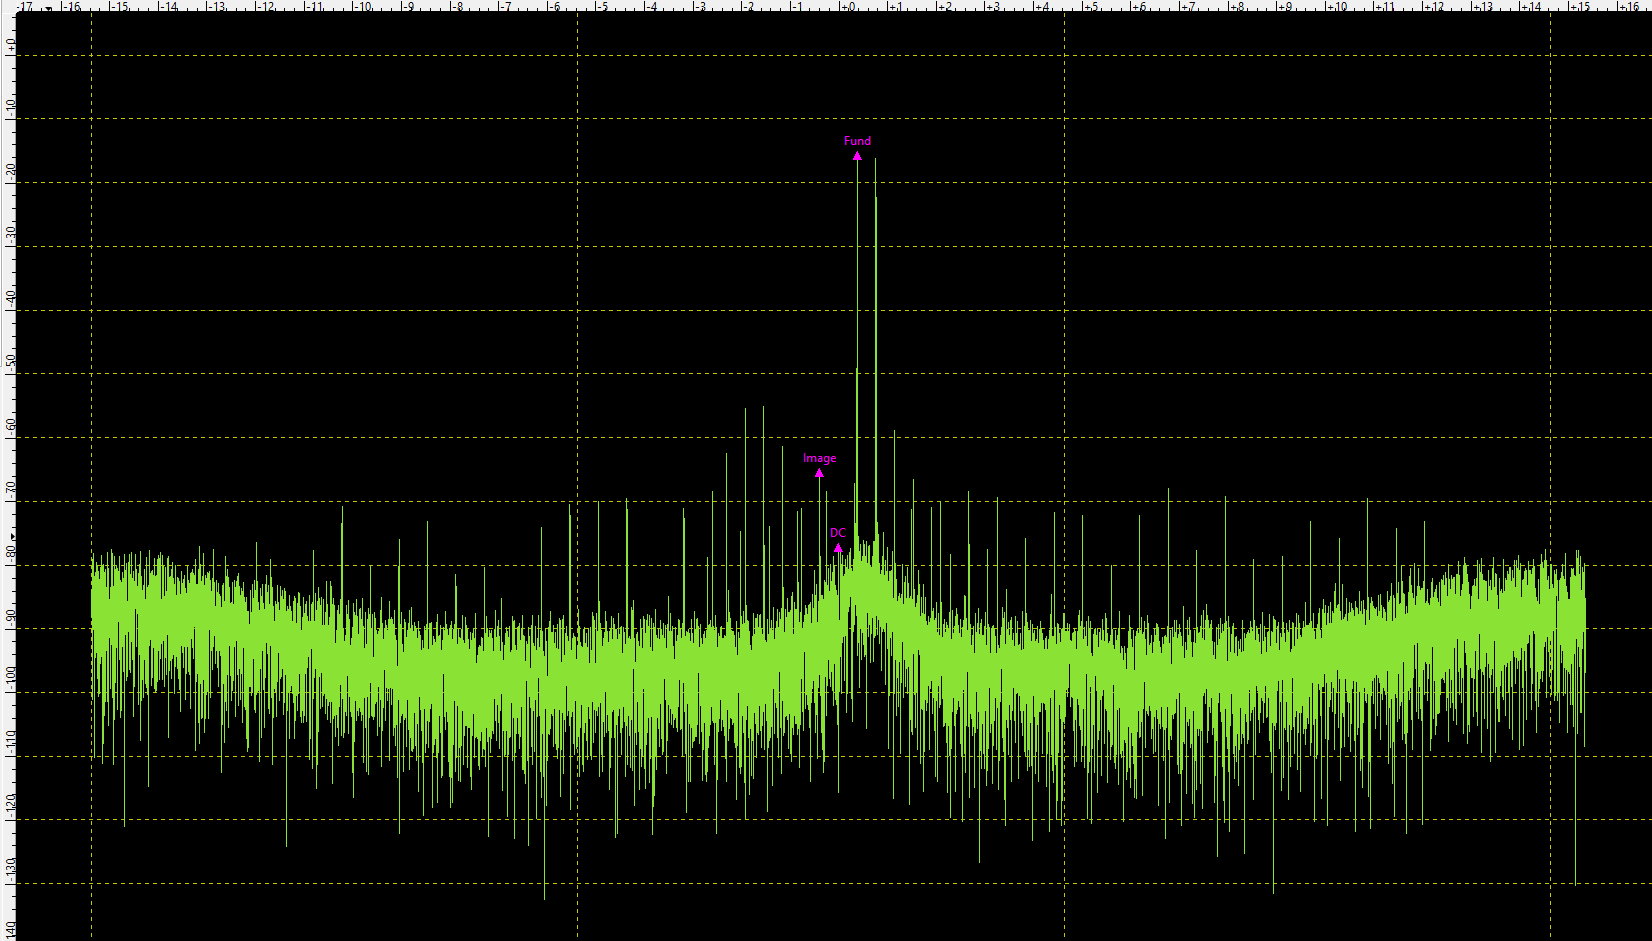
\includegraphics[width=\textwidth]{plots/my_multi_mav.png}
   		 	\caption{\textit{Received multi tone signal spectrum with IQ mismatch compensation with
   		 	Moving Average Filter.}}
   		\end{figure}	
   		
   		\begin{figure}[!htb]
    		\centering
   			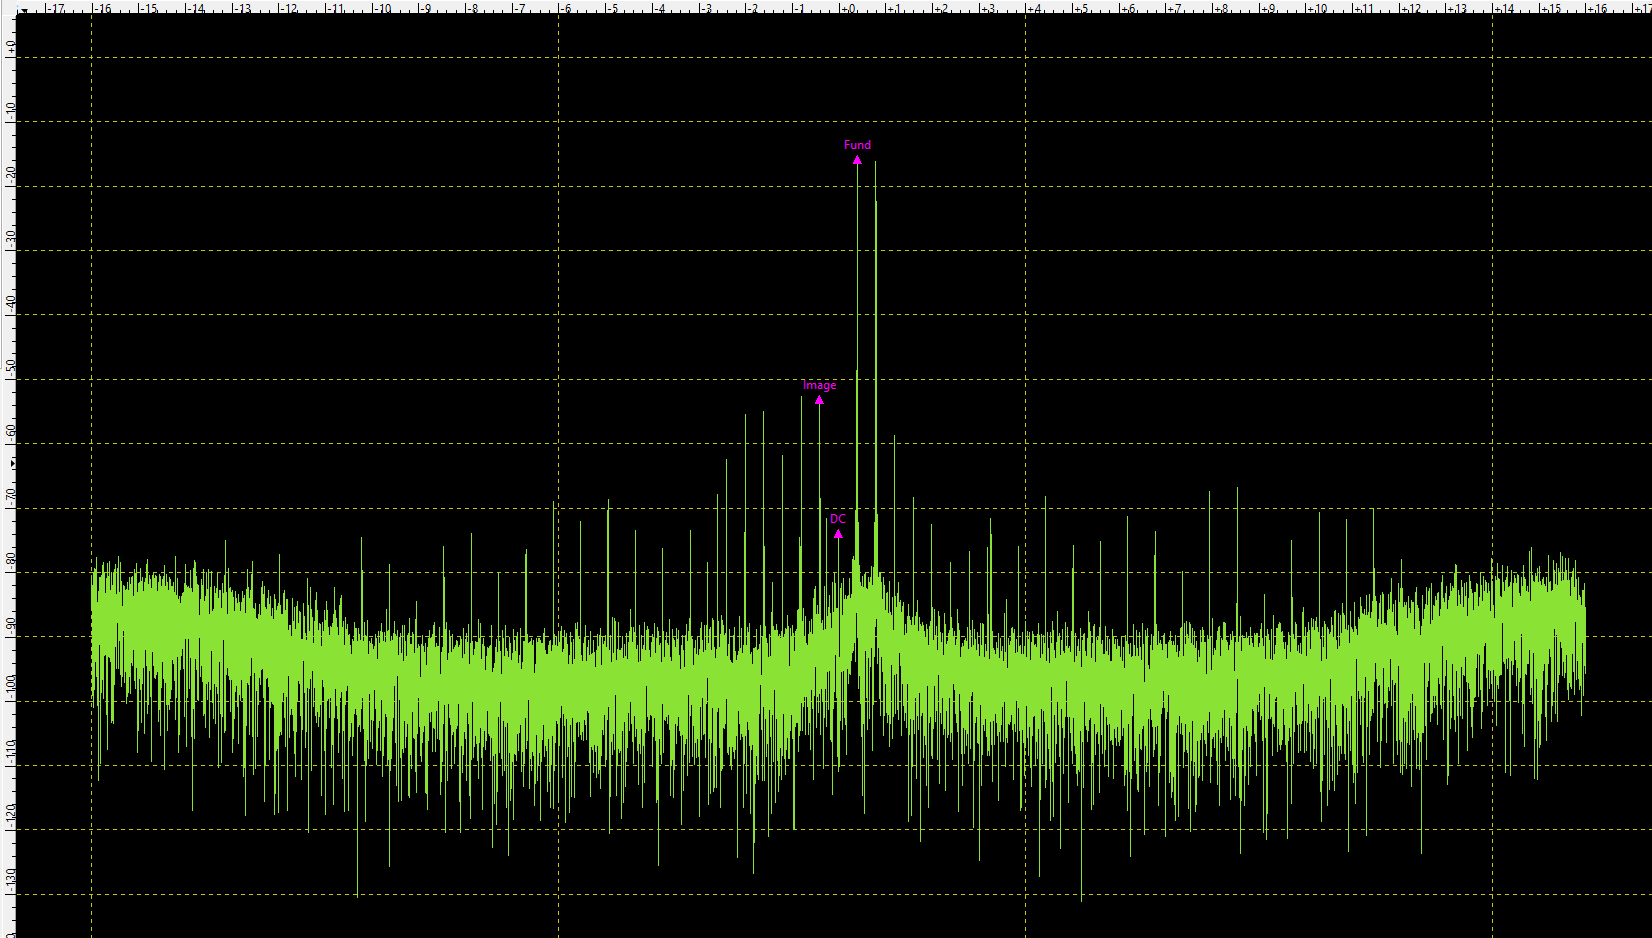
\includegraphics[width=\textwidth]{plots/my_multi_gauss.png}
   		 	\caption{\textit{Received broadband signal spectrum with IQ mismatch compensation with
   		 	Gaussian Filter.}}
   		\end{figure}		
		\subsection*{Broadband Signal}
		In this case implemented mismatch compensation is tested for
		broadband signal in frequency range from $f_s=0.5kHz$ to $f_e=1kHz$.
		\begin{figure}[!htb]
    		\centering
   			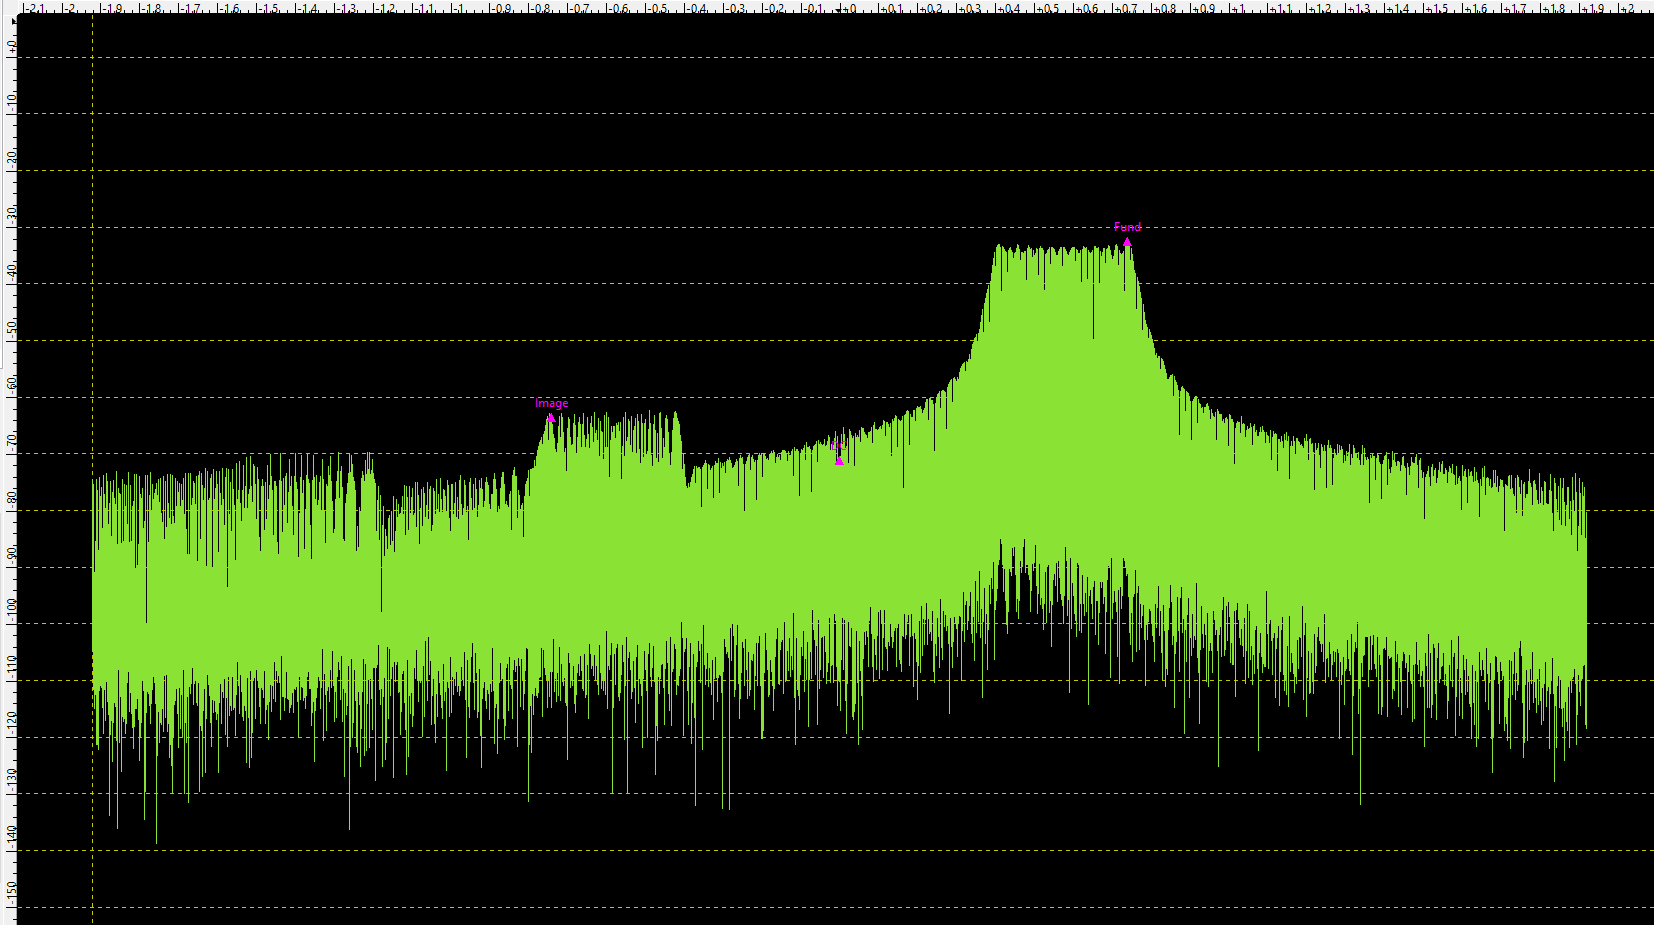
\includegraphics[width=\textwidth]{plots/my_band_mav.png}
   		 	\caption{\textit{Received broadband signal spectrum with IQ mismatch compensation with
   		 	Moving Average Filter.}}
   		\end{figure}
   		
   		\begin{figure}[!htb]
    		\centering
   			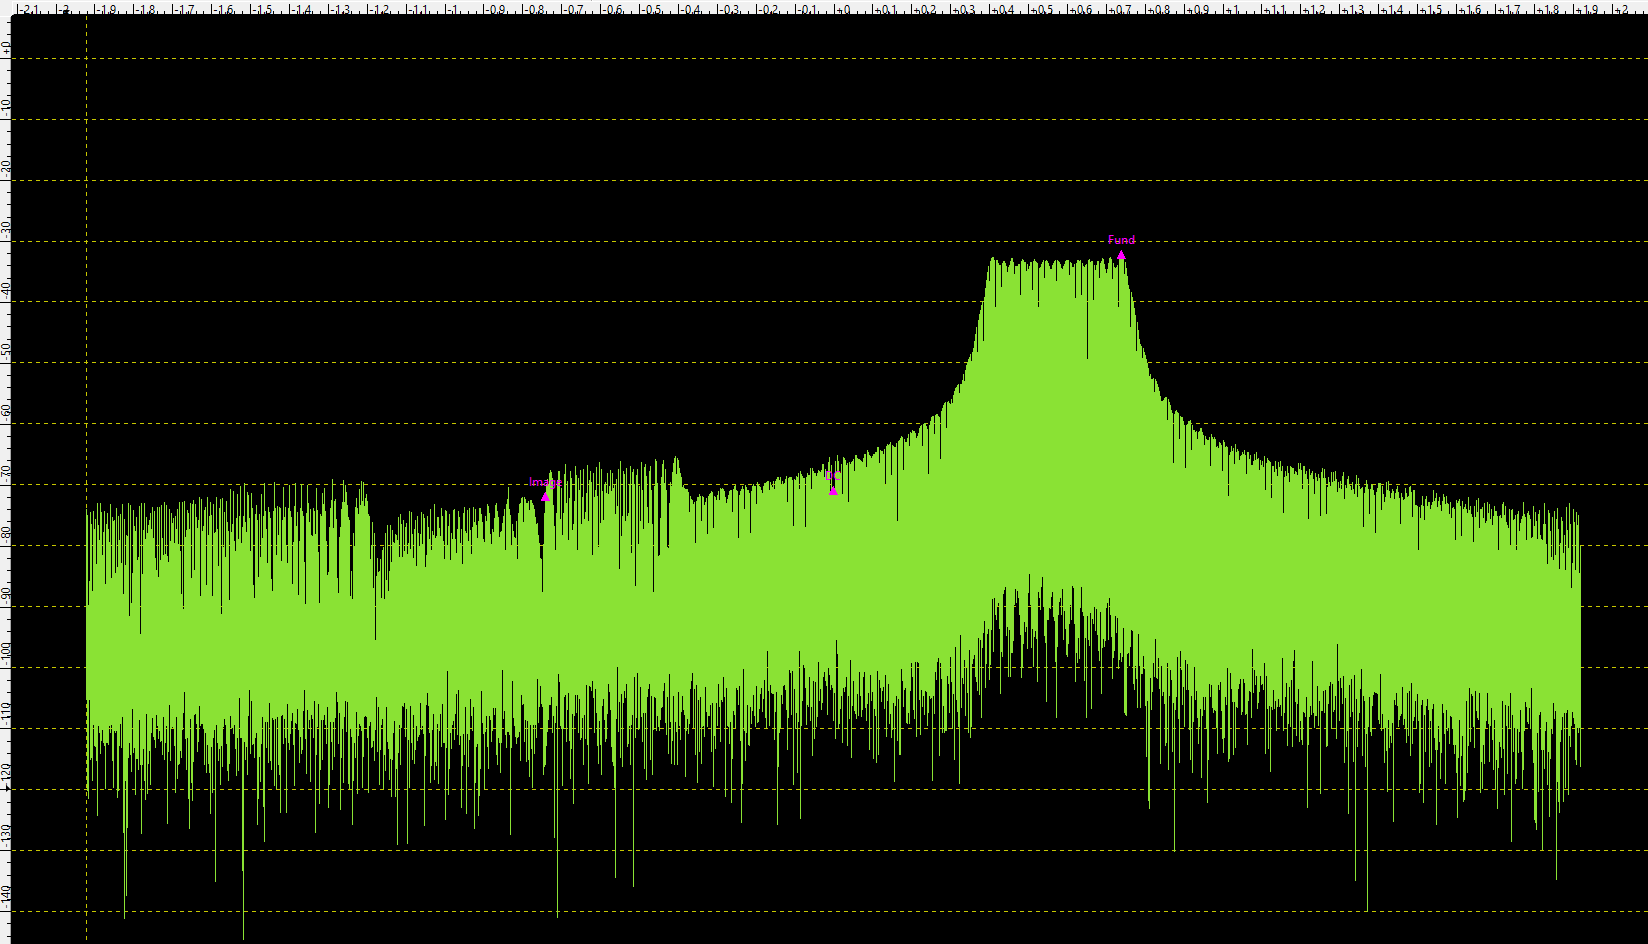
\includegraphics[width=\textwidth]{plots/my_band_gauss.png}
   		 	\caption{\textit{Received broadband signal spectrum with IQ mismatch compensation with
   		 	Gaussian Filter.}}
   		\end{figure}
   		
   		\newpage
		In all cases DC offset was successfully removed. Gaussian filter introduce additional spectral
		leakage close to the tone frequencies. Algorithms perform the worst in multi tone signal case.
		For single tone and broad band images are successfully reduced to almost level of the noise.	
   		
	\section{On Chip Algorithm}
		This section contains performance evaluation of compensation algorithms built in AD9363.
	
		All test were performed using IIO Oscilloscope program.
		Transmit and receive path are configured as follows:
		\begin{itemize}
			\item sampling rate - $30.719998$ MSPS,
			\item bandwidth - $18MHz$.,
			\item TX LO frequency - $2799.999998$ MHz,
			\item RX LO frequency - $2799.999998$ MHz.
		\end{itemize}

		\begin{itemize}
			\item Moving Average Filter Order - 256.
			\item Gaussian filter $\sigma$ = 5, window size = 30
			\item Amplitude - 1,
			\item DC offset in I branch - 0.1,
			\item Phase mismatch - 3$^\circ$.
		\end{itemize}
	    \newpage
		\subsection*{DC offset removal}
	 	In this case built in DC offset correction algorithm is tested for signle tone
		signal of frequency $f=1kHz$.				
   		 	\begin{figure}[!htb]
    			\centering
   				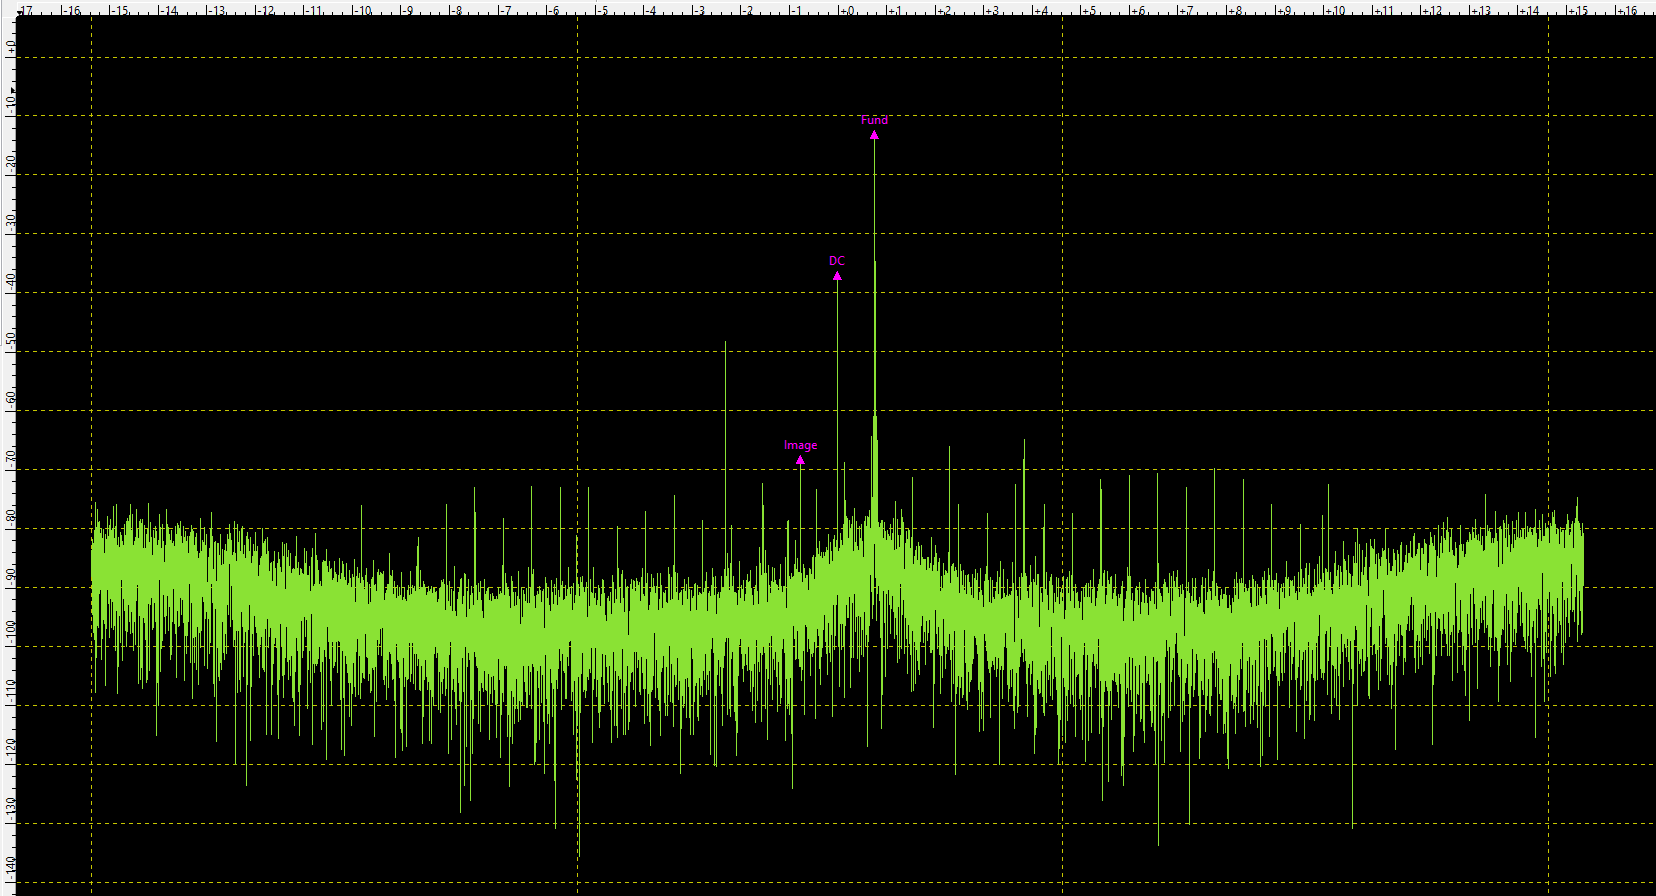
\includegraphics[width=\textwidth]{plots/real_dcoff.png}
   		 		\caption{\textit{Received signal spectrum without DC offset removal.}}
   		 	\end{figure}
   		 	\vspace{0.5cm}
   		 	\begin{figure}[!htb]
    			\centering
   				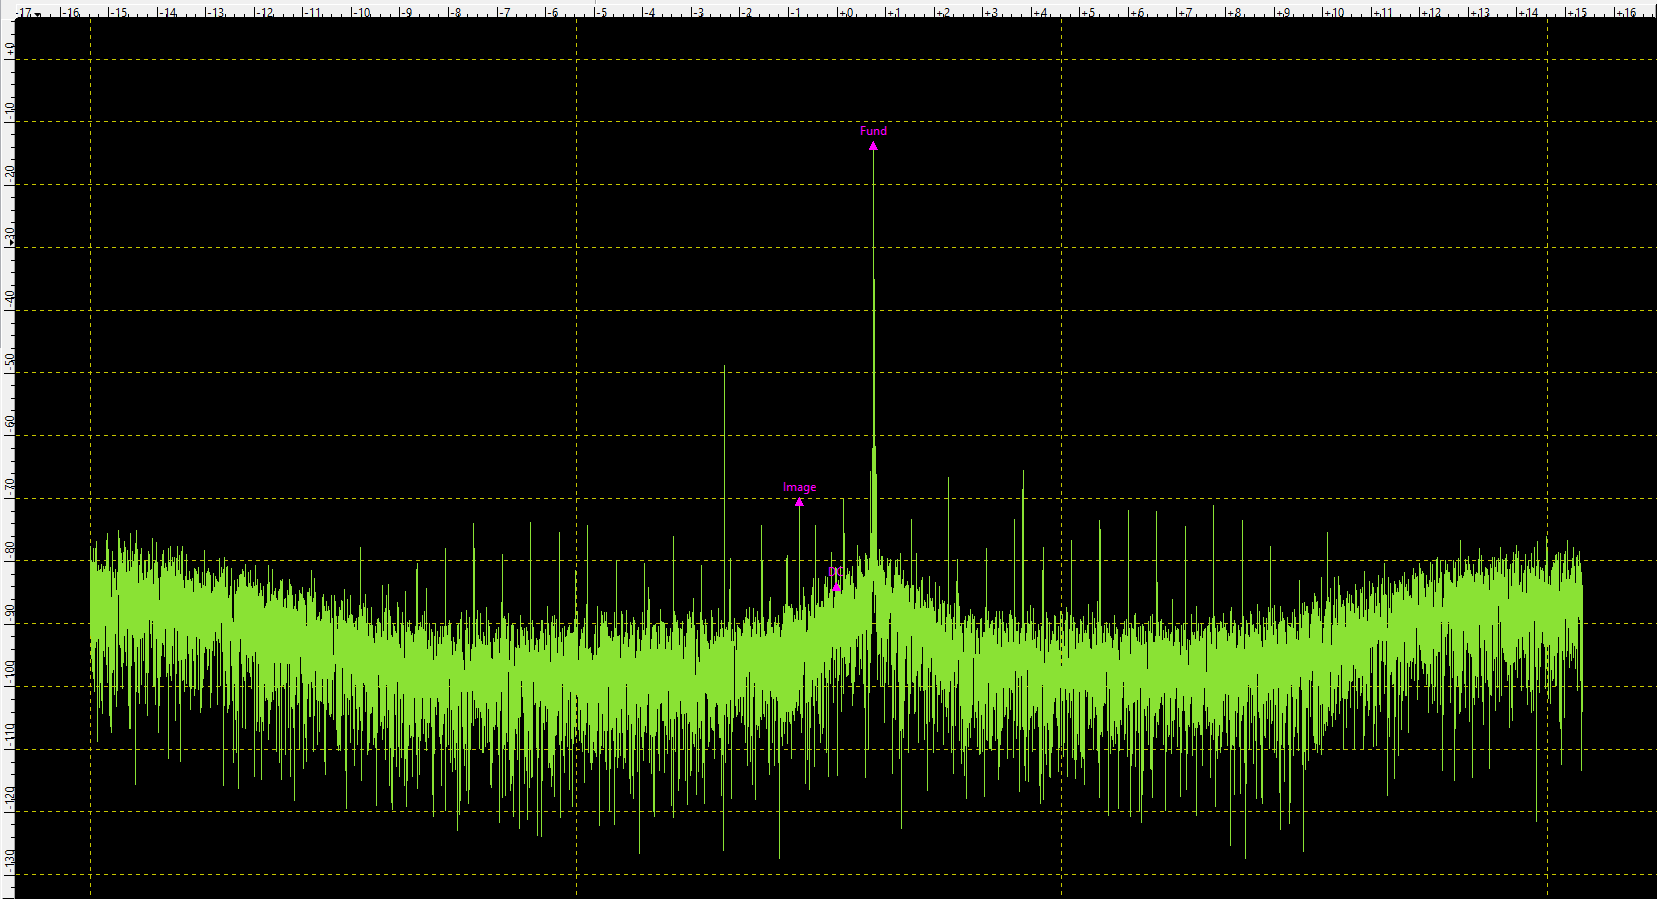
\includegraphics[width=\textwidth]{plots/real_dcon.png}
   		 		\caption{\textit{Received signal spectrum with AD9363 built in DC offset removal.}}
   		 	\end{figure}
   		\newpage
		\subsection*{Single Tone Signal}
		In this case built in IQ mismatch compensation and DC offset removal algorithms are
	 	tested for
		single tone signal with frequency $f=1kHz$.
		\begin{figure}[H]
    			\centering
   				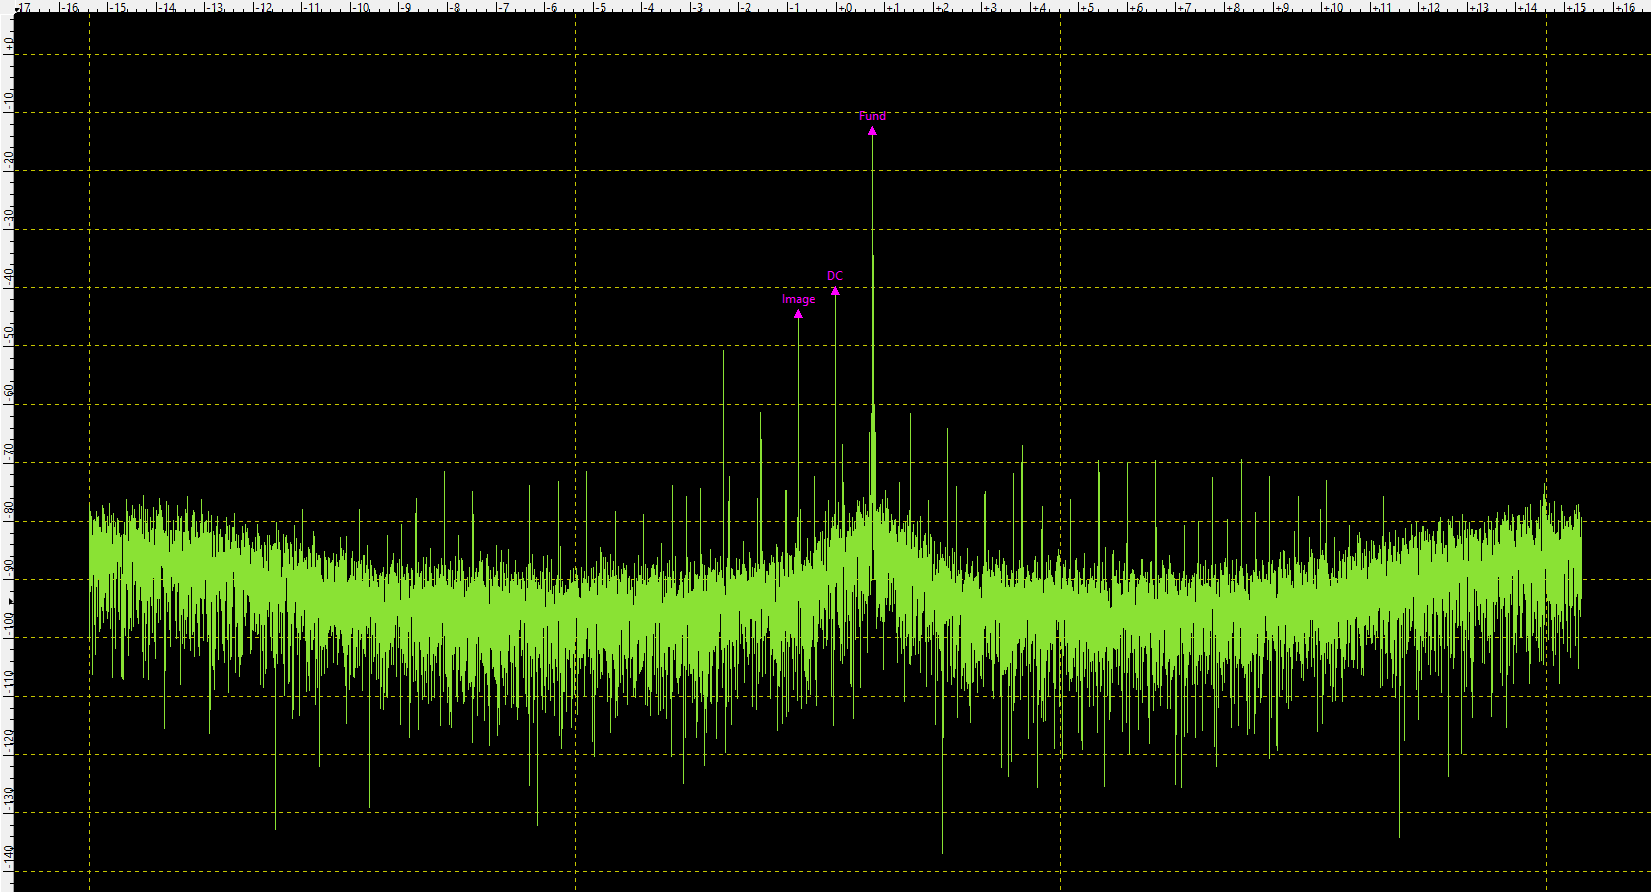
\includegraphics[width=\textwidth]{plots/real_single_off.png}
   		 		\caption{\textit{Received single tone signal spectrum without IQ mismatch compensation.}}
   		 	\end{figure}
			\vspace{0.5cm}
   		 	\begin{figure}[H]
    			\centering
   				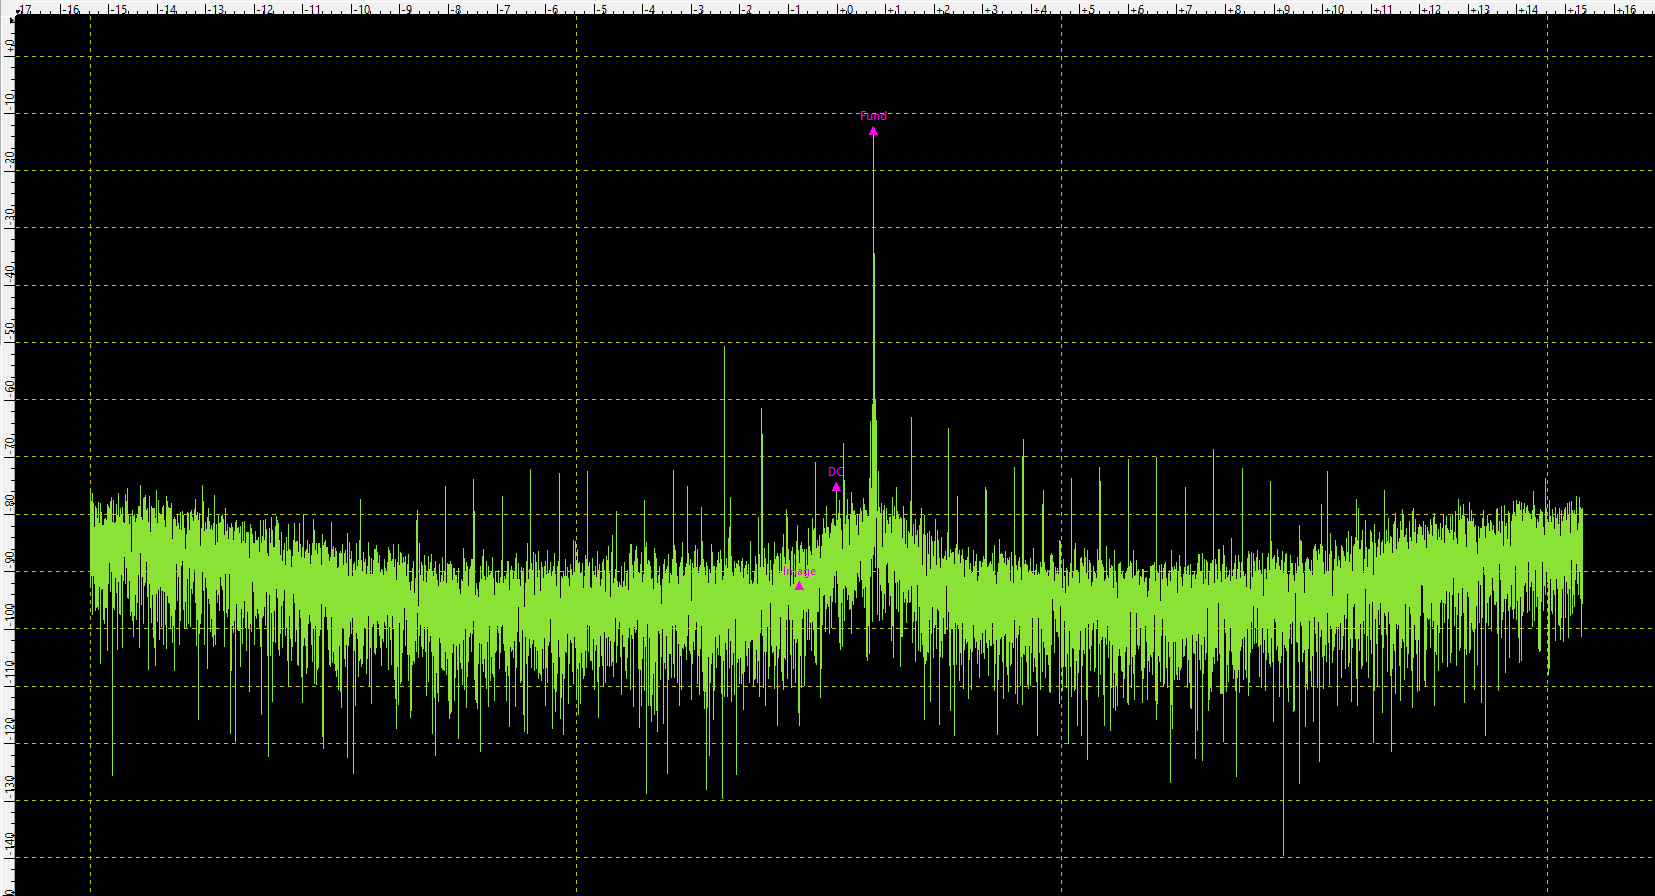
\includegraphics[width=\textwidth]{plots/real_single_on.png}
   		 		\caption{\textit{Received single tone signal spectrum with IQ mismatch compensation.}}
   		 	\end{figure}
   		\newpage
   	\subsection*{Multiton Signal}
   		In this case built in IQ mismatch compensation and DC offset removal algorithms are
	 	tested for multi signal with frequencies $f1=1kHz$ and $f2=0.5kHz$.
   		 	\begin{figure}[H]
    			\centering
   				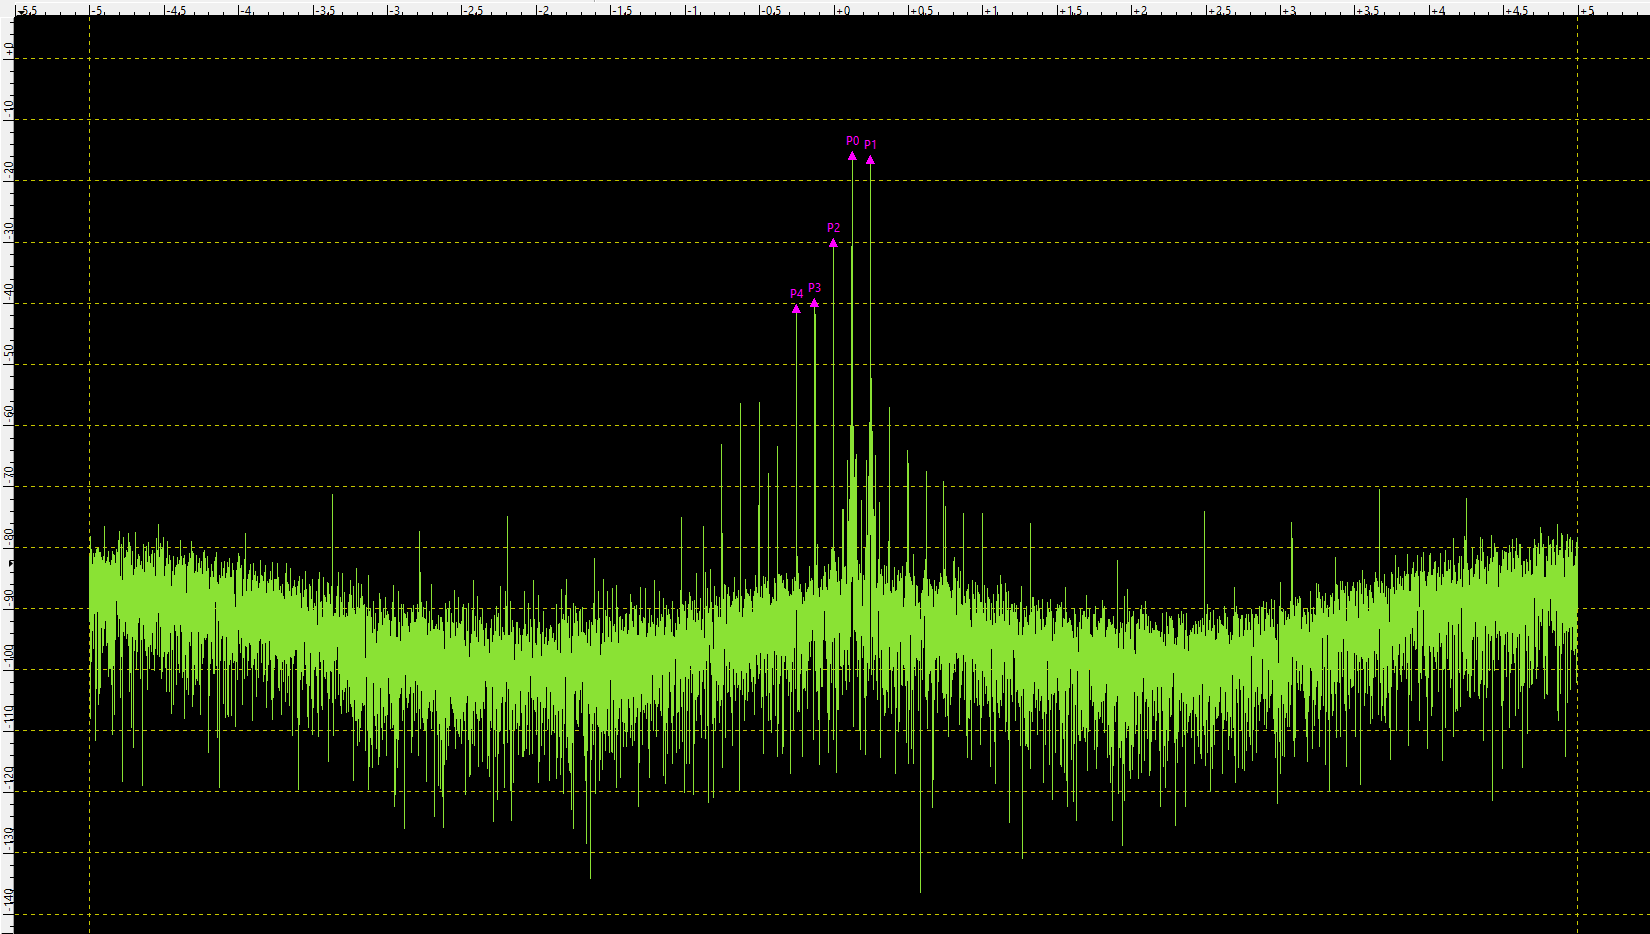
\includegraphics[width=\textwidth]{plots/real_multi_off.png}
   		 		\caption{\textit{Received multi tone signal spectrum without IQ mismatch compensation.}}
   		 	\end{figure}
   		 	\vspace{0.5cm}
   		 	\begin{figure}[H]
    			\centering
   				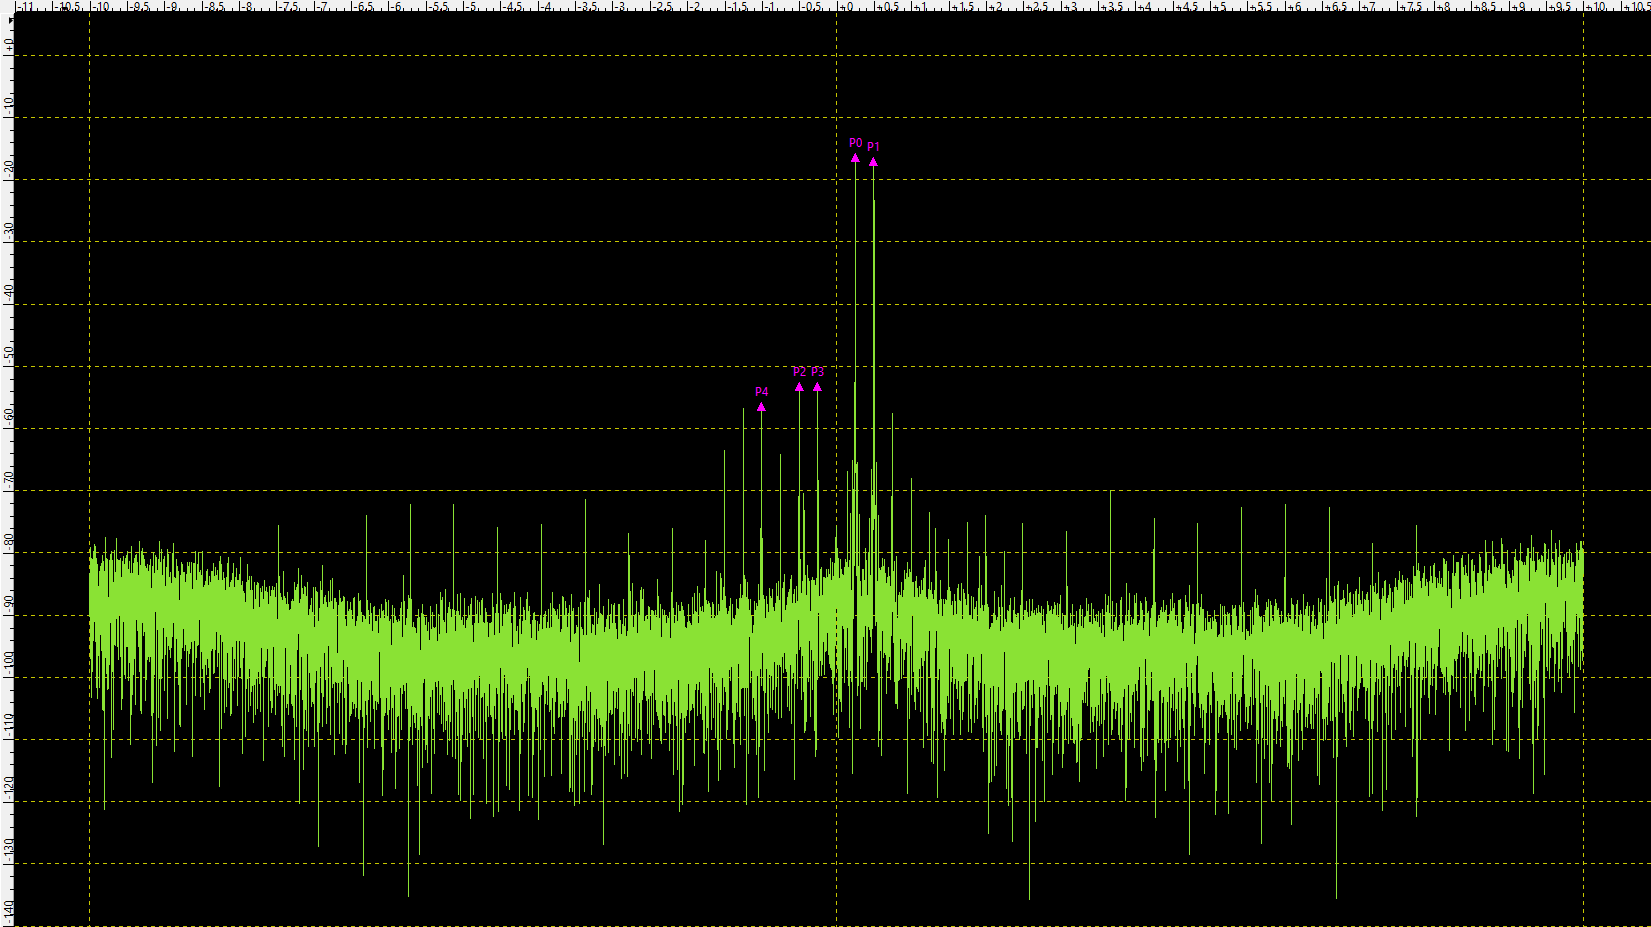
\includegraphics[width=\textwidth]{plots/real_multi_on.png}
   		 		\caption{\textit{Received multi tone signal spectrum with IQ mismatch compensation.}}
   		 	\end{figure}
   	 \newpage	
	 \subsection*{Broadband Signal}
	 	In this case built in IQ mismatch compensation and DC offset removal algorithms are
	 	tested for broadband signal in frequency range from $f_s=0.5kHz$ to $f_e=1kHz$.
   		 	\begin{figure}[H]
    			\centering
   				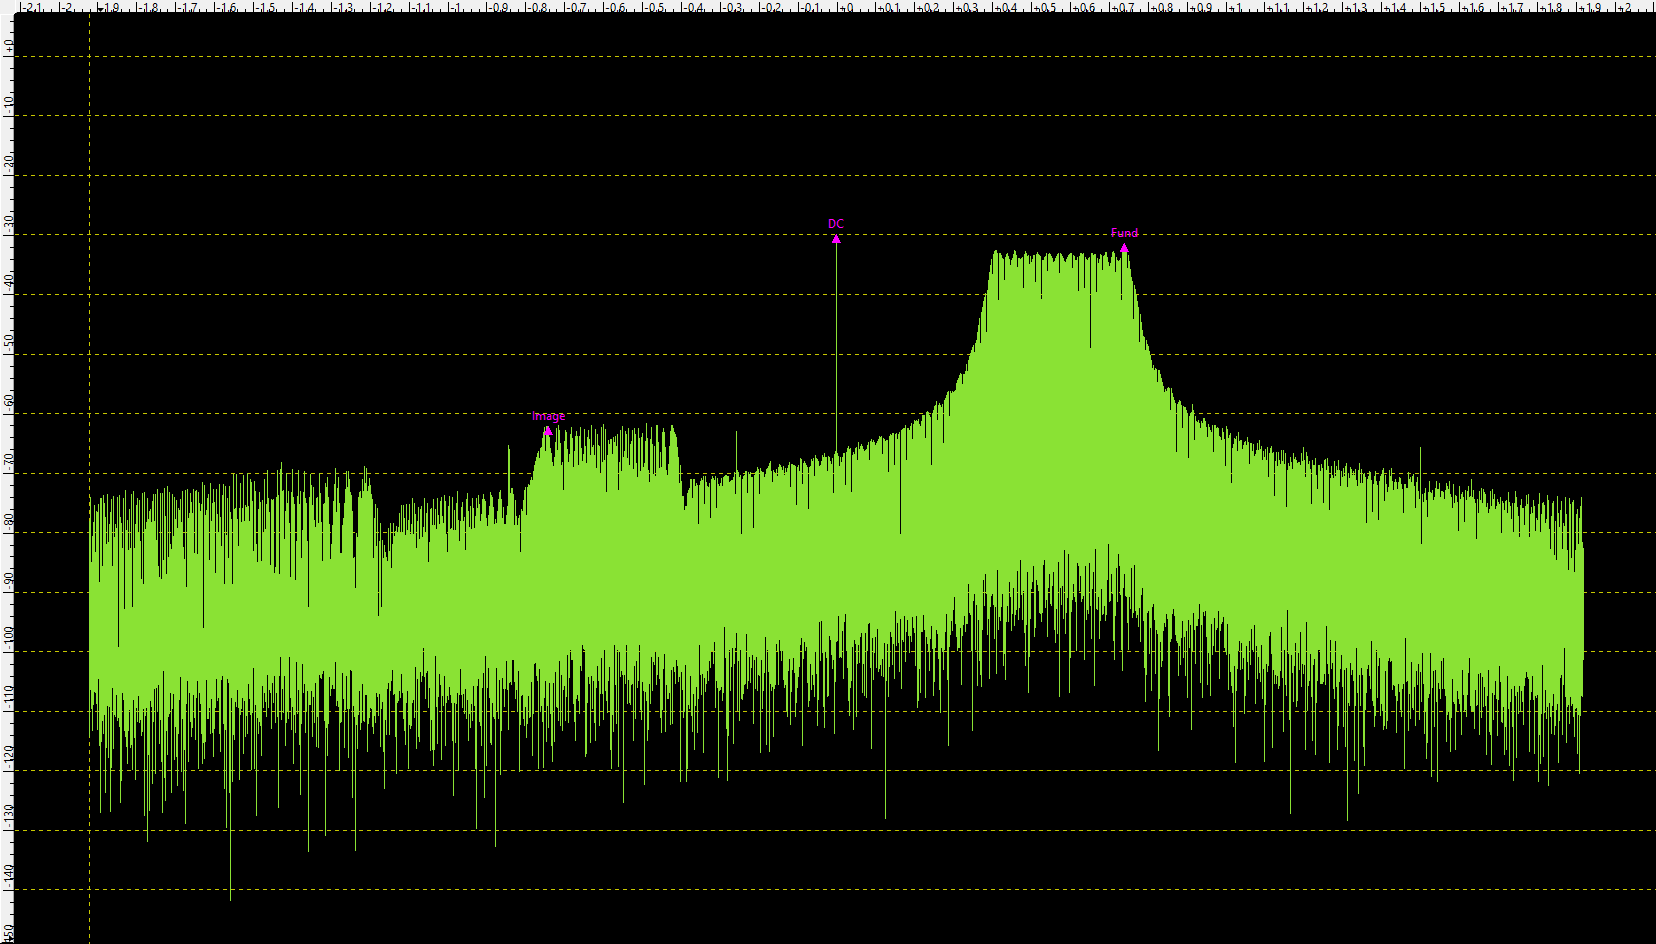
\includegraphics[width=\textwidth]{plots/real_band_off.png}
   		 		\caption{\textit{Received broadband signal spectrum without IQ mismatch compensation.}}
   		 	\end{figure}
   		 	\vspace{0.5cm}
   		 	\begin{figure}[H]
    			\centering
   				\includegraphics[width=\textwidth]{plots/real_band_on.png}
   		 		\caption{\textit{Received broadband signal spectrum with IQ mismatch compensation.}}
   		 	\end{figure}
   		 	\newpage
   		 	In all cases DC offset component was successfully removed.  		 	
			For multi tone singal test case markers P0 and P1 represents $1kHz$ and $0.5kHz$ 
			tons in the signal. P3 and P4 are images
   		 	of P0 and P1. P2 marker is DC component in the signal. In this case built in algorithms
   		    performance was the worst. Image fringes were reduced by only 10dB. For broadband signal
   		    image was reduced to the level of noise.
   		    
\chapter{ Conclusions}
	Performance of presented algorithms was very satisfying. In all cases test cases DC component was
	successfully removed form the signal. Gaussian filter takes more resources than Moving Average
	Filter, but requires almost 9 times lower number of samples to operate (256 samples in case of 
	Moving Average Filter and 30 for Gaussian Filter). Gaussian filter introduced additional spectral
	leakage close to signal tone frequency. Gaussian Filter worked better for multi tone signal
	than Moving Average but was worse in case of broadband signal.
	In all cases unwanted images were significantly reduced.
	Constellation diagram shapes are closer to circle which means orthogonality of the I and Q component.
	In case of single tone signal constellation diagram changes it shape form ellipse to circle. For
	multi tone two circles are present. One for lower and one for higher frequency tone. Broadband signal
	constellation diagram is a ring with lower bound at lowest frequency in the band ad upper bound in
	the highest. Introduction of the noise confirmed that algorithms are able to work in real case. 
	However performance of both implemented and built in algorithm for multi tone
	signal case was the worst. Performance of algorithms implemented in Zynq PL section was better than
	built in AD9363 transceiver for single and multi tone, but worse for broadband signal.	
	\\
	
	
	Algorithms tested in this thesis shows that it is possible to significantly improve RF signal
	quality using both implementation approaches: in software and in hardware. However hardware
	approach allowed to perform effective IQ correction in real time. Devices such as SoC shows
	potential in field of SDR, thanks to mixed architecture of CPU and FPGA.


\addcontentsline{toc}{chapter}{Bibliography} %utworzenie w spisie treści pozycji Bibliografia
\bibliography{bibliografia} % wstawia bibliografię korzystając z pliku bibliografia.bib - dotyczy BibTeXa, jeżeli nie korzystamy z BibTeXa należy użyć otoczenia thebibliography

\begin{thebibliography}{9}
\bibitem{lyo}
R.G Lyons
\textit{„Wprowadzenie do cyfrowego przetwarzania sygnałów, WKiŁ, 1999}

\bibitem{iqcorr} 
S.W. Ellingson. 
\textit{Correcting I-Q Imbalance in Direct Conversion
Receivers, February 10, 2003}.

\bibitem{iq_model}
Lauri Anttila,
Mikko Valkama,
Markku Renfors
\textit{Frequency-Selective I/Q Mismatch Calibration of Wideband Direct-Conversion Transmitters, https://ieeexplore.ieee.org/abstract/document/4476448}

\bibitem{iq_imball}
Guanbin Xing, Manyuan Shen, Hui Liu.
\textit{Frequency Offset and I/Q Imbalance Compensation for Direct-Conversion Receivers. IEEE TRANSACTIONS ON WIRELESS COMMUNICATIONS, VOL. 4, NO. 2, MARCH 2005.}

\bibitem{filter_design}
T. W. Parks,
C. Sidney Burrus
\textit{Digital Signal Processing and
Digital Filter Design, Wiley-Interscience; 1 edition (August 1987)}
\bibitem{comp}
François Horlin, André Bourdoux
\textit{Digital Compensation for
Analog Front-Ends. England: 2008 John Wiley & Sons, Ltd}


\bibitem{mav}
Steven W. Smith, Ph.D.
\textit{The Scientist and Engineer's Guide to
Digital Signal Processing. https://www.analog.com/media/en/technical-documentation/dsp-book/dsp_book_Ch15.pdf}

\bibitem{zynq_book}
Louise H. Crockett
Ross A. Elliot
Martin A. Enderwitz
Robert W. Stewart
\textit{The Zynq Book Embedded Processing with the ARM® Cortex®-A9 on the Xilinx®
Zynq®-7000 All Programmable SoC, Department of Electronic and Electrical Engineering
University of Strathclyde
Glasgow, Scotland, UK
1st Edition}

\bibitem{hls}
Xilinx Inc.,
\textit{Vivado Design Suite User Guide - High-Level Synthesis. https://www.xilinx.com/support/documentation/sw_manuals/xilinx2017_4/ug902-vivado-high-level-synthesis.pdf}

\bibitem{hls2}
Xilinx Inc.,
\textit{Xilinx Vivado High Level Synthesis: Case studies, https://digital-library.theiet.org/content/conferences/10.1049/cp.2014.0713}

\bibitem{zynq_ds}
Xilinx Inc.,
\textit{Zynq-7000 SoC Data Sheet, https://www.xilinx.com/support/documentatio \\
n/data_sheets/ds190-Zynq-7000-Overview.pdf}

\bibitem{zynq_manual}
Xilinx Inc.,
\textit{Zynq-7000 SoC Technical Reference Manual, https://www.xilinx.com/support/documentation/user_guides/ug585-Zynq-7000-TRM.pdff}
\bibitem{ad9363}
Analog Devices Inc.,
\textit{AD9363 Datasheet, https://www.analog.com/media/en/technical-documentation/data-sheets/AD9363.pdf}

\bibitem{zynq_guide}
Xilinx Inc.,
\textit{Zynq-7000 All
Programmable SoC
Software Developers Guide, https://www.xilinx.com/support/documentation/user_guides/ug821-zynq-7000-swdev.pdf}

\bibitem{pluto_photo}
\textit{https://www.analog.com/-/media/analog/en/evaluation-board-images/images/adalm-pluto-web.gif?h=270&thn=1&hash=A9C5189745767A0191C4536 \\
A230C498745F14619}

\bibitem{pluto_schematic}
\textit{https://www.analog.com/-/media/analog/en/evaluation-board-images/images/adalm-pluto_medium_block_diagram.png?h=270&hash=1A0512F2EC \\
9F8DAA40A1C954A2394FE4E8BA34B3}

\bibitem{ad9363_diag}
\textit{http://analogdevicesinc.github.io/libad9361-iio/doc/AD9361.svg}

\bibitem{zynq_diag}
\textit{https://www.cnx-software.com/wp-content/uploads/2012/03/xilinx_zynq-7000_EPP_block_diagram_large.jpg}
\bibitem{libioo}
\textit{https://wiki.analog.com/_detail/resources/tools-software/linux-software/libiio_diagram.png?id=resources\%3Atools-software\%3Alinux-software\%3Alibiio}
\end{thebibliography}
%opcjonalnie może się tu pojawić spis rysunków i tabel
% \listoffigures
% \listoftables
\end{document}
